\documentclass[11pt,oneside]{book}

\usepackage{xcolor}
\usepackage{mathtools}
\usepackage[legalpaper, margin=1in]{geometry}
\usepackage{amsmath}
\usepackage{amssymb}
\usepackage{paralist}
\usepackage{rsfso}
\usepackage{amsthm}
\usepackage[inline]{enumitem}   

\newtheoremstyle{break}
  {\topsep}{\topsep}%
  {\itshape}{}%
  {\bfseries}{}%
  {\newline}{}%
\theoremstyle{break}
\theoremstyle{break}
\newtheorem{axiom}{Axiom}
\newtheorem{thm}{Theorem}[section]
\newtheorem{lem}{Lemma}[thm]
\newtheorem{prop}[lem]{Proposition}
\newtheorem{corL}{Corollary}[lem]
\newtheorem{corT}[lem]{Corollary}
\newtheorem{defn}{Definition}[corL]

\newcommand{\R}{\mathbb{R}}
\newcommand{\N}{\mathbb{N}}
\newcommand{\Z}{\mathbb{Z}}
\newcommand{\Q}{\mathbb{Q}}
\newcommand{\A}{\mathcal{A}}
\newcommand{\J}{\mathcal{J}}
\newcommand{\T}{\mathcal{T}}
\newcommand{\C}{\mathcal{C}}
\newcommand{\M}{\mathcal{M}}
\newcommand{\khat}{\hat{\text{k}}}
\newcommand{\Complex}{\mathbb{C}}
\newcommand{\Power}{\mathcal{P}}
\newcommand{\pd}{\partial}
\newcommand{\ee}[1]{\cdot 10^{#1}}
\newcommand{\bmat}[1]{\begin{bmatrix}
#1
\end{bmatrix}}
\newcommand{\ihat}{\hat{\i}}
\newcommand{\jhat}{\hat{\j}}


\newcommand{\note}{\color{red}Note: \color{black}}
\newcommand{\remark}{\color{blue}Remark: \color{black}}
\newcommand{\example}{\color{green}Example: \color{black}}
\newcommand{\exercise}{\color{green}Exercise: \color{black}}




\makeatletter
\def\@seccntformat#1{%
  \expandafter\ifx\csname c@#1\endcsname\c@section\else
  \csname the#1\endcsname\quad
  \fi}
\makeatother

\makeatletter
\newcommand*{\rom}[1]{\expandafter\@slowromancap\romannumeral #1@}
\makeatother

\makeatletter
% This command ignores the optional argument for itemize and enumerate lists
\newcommand{\inlineitem}[1][]{%
\ifnum\enit@type=\tw@
    {\descriptionlabel{#1}}
  \hspace{\labelsep}%
\else
  \ifnum\enit@type=\z@
       \refstepcounter{\@listctr}\fi
    \quad\@itemlabel\hspace{\labelsep}%
\fi}
\makeatother
\parindent=0pt


\begin{document}

	\begin{titlepage}
		\begin{center}
			\topskip0pt
			\vspace*{\fill}
			\Huge \color{red}
				\textbf{Class Note}\\
			\vspace{0.5cm}			
			\Large \color{black}
				Physics 401 - Classical Mechanics\\	
				Professor Bing Zhou\\
				University of Michigan\\
			\vspace{3cm}
			
			\begin{center}
			
\includegraphics[scale=0.8]{hmm.pdf}
			\end{center}
			
			\vspace{3cm}
			\LARGE
				\textbf{Jinyan Miao}\\
				Winter 2022\\
			\vspace{5cm}

		\vspace*{\fill}
		\end{center}			
	\end{titlepage}

\tableofcontents
\addtocontents{toc}{~\hfill\textbf{Page}\par}

\newpage
\chapter{Math Review}
\section[Vector Calculus]{\color{red} Vector Calculus\color{black}}
A \textbf{vector field}, denoted as $f(\vec{r},t)$, is a function of space-time $(\vec{r},t)$, and it is a function specified by a direction and magnitude. More precisely, a vector field is defined by its transformation properties under the coordinate system rotation. Physics laws should be independent from the selected coordinate system. \\

A \textbf{scalar field}, denoted as $\psi(\vec{r},t)$, is a function of space-time $(\vec{r},t)$, and it is a spatial function specified only by its magnitude, independent of direction.\\

The set of \textbf{base vectors} for Cartesian coordinate system, denoted as $\{\hat{x},\hat{y}, \hat{z}\}$, consists of unitary vectors pointing in the $x$, $y$, $z$ directions respectively. The base vectors are orthogonal to each other, following the right hand rule.\\

A \textbf{coordinate system} is defined by its base vectors and the origin. 

For $\vec{A},\vec{B},\vec{C} \in \R^3$, we have the followings:
\begin{enumerate}
\item $\vec{A}\cdot (\vec{B}\times \vec{C}) = \vec{B}\cdot (\vec{C}\times \vec{A}) = \vec{C}\cdot (\vec{A}\times \vec{B})$ is the volume of a parallelpiped formed by $\vec{A},\vec{B},\vec{C}$
\item $\vec{A}\times (\vec{B}\times \vec{C}) = \vec{B}(\vec{A}\cdot \vec{C}) - \vec{C}(\vec{A}\cdot \vec{B})$
\end{enumerate}

Newton's Law:
\begin{enumerate}
\item First Law states that if no net force acting on the system, then the velocity of the system is constant. That is, if $\sum \vec{F}_i = 0$, then $\vec{v}$ is a constant vector. 
\item Second Law states that $\vec{F} = m\vec{a} = m\frac{d\vec{v}}{dt} = m\frac{d^2\vec{r}}{dt^2}$, where $\vec{v} = \frac{d\vec{r}}{dt}$, and $\vec{a} = \frac{d^2\vec{r}}{dt}$.
\item Third Law, or the Action and Reaction Law, states that $F_{i\to j} = -F_{j \to i}$. 
\end{enumerate}


\subsection*{Cylindrical and Spherical Coordinate Systems}
Here we use $\phi$ to denote the angle on the $xy$-plane from the positive $x$-axis, and $\theta$ to denote the angle from the vertical positive $z$-axis, as shown by the following diagram:\\
\begin{center}
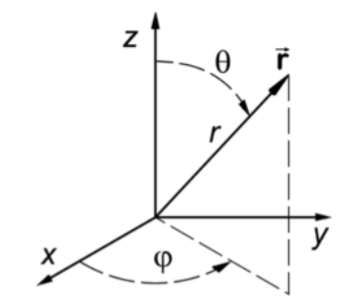
\includegraphics[scale=0.5]{thetaAndPhi.png}
\end{center}


For transformation between cylindrical coordinate and Cartesian coordinate, we have the followings:
$$\hat{r} = \hat{x}\cos(\phi) + \hat{y}\sin(\phi),\quad \hat{\phi} = -\hat{x}\sin(\phi) + \hat{y}\cos(\phi),\quad \hat{z}=\hat{z}$$
$$\hat{x} = \hat{r}\cos(\phi) - \hat{\phi}\sin(\phi),\quad \hat{y}=\hat{r}\sin(\phi) + \hat{\phi}\cos(\phi),\quad \hat{z} = \hat{z}$$
By Chain Rule, we get the following:
$$\frac{d\hat{r}}{dt} = \hat{x}\,(-\sin(\phi)\dot{\phi}) + \hat{y}\,(\cos(\phi)\dot{\phi}) = \dot{\phi}\,\hat{\phi} \qquad\qquad\frac{d\hat{\phi}}{dt} = \hat{x}\,(-\cos(\phi)\dot{\phi})+ \hat{y}\,(-\sin(\phi) \dot{\phi}) = -\dot{\phi}\,\hat{r}$$
Note that $\hat{x},\hat{y},\hat{z}$ are position independent, while $\hat{\phi}$ and $\hat{r}$  are position dependent. \footnote{The basis vector $\hat{r}$ is sometimes denoted as $\hat{\rho}$, or $\hat{s}$.}\\

In general, we have the following transformation between Cartesian and cylindrical coordinate:
$$r = \sqrt{x^2 + y^2} \qquad \qquad \phi = \tan^{-1}\left(\frac{y}{x} \right)\qquad\qquad z=z$$
$$x = r \cos(\phi) \qquad\quad\, \qquad y=r \sin(\phi) \qquad\qquad\quad\,  z=z$$

\hfill\break
For transformation between the spherical coordinate and Cartesian coordinate, we have:
\begin{align*}
&\hat{r} = \hat{x}\sin(\theta) \cos(\phi) + \hat{y}\sin(\theta) \sin(\phi) + \hat{z}\cos(\theta)\\
&\hat{\theta} = \hat{x}\cos(\theta) \cos(\phi) + \hat{y}\cos(\theta)\sin(\phi)  - \hat{z}\sin(\theta) \\ 
&\hat{\phi} = -\hat{x}\sin(\phi) + \hat{y}\cos(\phi)
\end{align*}
\begin{align*}
&\hat{x} = \hat{r}\sin(\theta)\cos(\phi) + \hat{\theta}\cos(\theta) \cos(\phi) - \hat{\phi}\sin(\phi)\\
&\hat{y} = \hat{r}\sin(\theta)\cos(\phi) + \hat{\theta}\cos(\theta)\sin(\phi) + \hat{\phi}\cos(\phi)\\
&\hat{z} = \hat{r}\cos(\theta) - \hat{\theta}\sin(\theta)
\end{align*}
Note that $\hat{x},\hat{y},\hat{z}$ are position independent, while $\hat{\phi}$,$\hat{\theta}$,$\hat{r}$ are position dependent.\\

From such relation one can derive the followings:
\begin{align*}
&\frac{d \hat{r}}{dt} = \dot{\theta}\, \hat{\theta} + \sin(\theta) \dot{\phi}\, \hat{\phi}\qquad\qquad \frac{d\hat{\theta}}{dt}=-\dot{\theta}\,\hat{r}+\cos(\theta)\dot{\phi}\, \hat{\phi}\qquad\qquad \frac{d\hat{\phi}}{dt} = -\sin(\theta)\dot{\phi}\,\hat{r} - \cos(\theta) \dot{\theta}\, \hat{\theta} 
\end{align*}

In general, for transformation between spherical and Cartesian coordinate, we write the following:
$$
x = r \sin(\theta) \cos(\phi) \qquad\qquad y = r \sin(\theta) \sin(\phi) \qquad\qquad z = r\cos(\theta)
$$
$$r = \sqrt{x^2 + y^2 + z^2} \qquad\qquad \theta = \tan^{-1}\left(\frac{y}{x} \right)\qquad\qquad \phi = \tan^{-1}\frac{\sqrt{x^2+y^2}}{z} = \cos^{-1}\frac{z}{\sqrt{x^2+y^2+z^2}}$$


\subsection*{Del Operator}
For a scalar function $T:\R^3 \to \R$, denoted as $T(x,y,z) = T(\vec{r})$. The change in $T$ from the position vector $\vec{r}$ to position vector $\vec{r}+ d\vec{r}$ is given by the following:
$$dT = \frac{\partial T}{\partial x}\,dx + \frac{\partial T}{\partial y}\,dy \frac{\partial T}{\partial z}\,dz = \left( \frac{\pd T}{\pd x}, \frac{\pd T}{\pd y}, \frac{\pd T}{\pd z}\right) \cdot (dx,dy,dz) = \nabla T \cdot d\vec{r}$$
Here $\nabla T$ is a vector and is called the gradient of function $T(\vec{r})$. Note that we have: 
$$dT = \nabla T\cdot d\vec{r} = |\nabla T|\, |d\vec{r}| \, \cos(\theta)$$ where $\theta$ is the angle between $\nabla T$ and $d\vec{r}$, so we see that $dT$ is maximum when $\theta  = 0$, and hence the gradient $\nabla T$ points in the direction of maximum change of function $T$, and its magnitude is the rate of increase along this direction. \\

Now we define the Del operator as the following:
$$\nabla \coloneqq \hat{x}\,\frac{\pd}{\pd x} + \hat{y} \,\frac{\pd}{\pd y}+ \hat{z}\,\frac{\pd}{\pd z}$$

The Divergence of a vector function $\vec{V} =  V_x \hat{x} + V_y \hat{y} + V_z \hat{z}$ is given by the following:
$$\nabla \cdot \vec{V} = \left(\hat{x}\,\frac{\pd}{\pd x} + \hat{y} \,\frac{\pd}{\pd y}+ \hat{z}\,\frac{\pd}{\pd z}\right) \cdot \left( V_x \hat{x} + V_y \hat{y} + V_z \hat{z}\right) = \frac{\pd V_x}{\pd x} + \frac{\pd V_y}{\pd y}+ \frac{\pd V_z}{\pd z}$$
Note that $\nabla \cdot V$ returns a scalar. The divergence is a measure of the spreadness of a vector function. A sink has negative divergence, and a faucet has positive divergence. \\

The Curl of a vector function $\vec{V} =  V_x \hat{x} + V_y \hat{y} + V_z \hat{z}$ is given by the following:
$$\nabla \times \vec{V} = \left( \frac{\pd V_z}{\pd y} - \frac{\pd V_y}{\pd z}\right) \hat{x} + \left( \frac{\pd V_x}{\pd z} - \frac{\pd V_z}{\pd x}\right) \hat{y} + \left( \frac{\pd V_y}{\pd x} - \frac{\pd V_x}{\pd y}\right) \hat{z}$$
Note that $\nabla \times \vec{V}$ returns a vector. Curl is a measure of the curlness, or rotation, of a vector function. The direction of the curl follows the right hand rule.\\

The Laplacian operator is the divergence of gradient. The divergence of gradient of a scalar function $T$ is given by the following:
$$\nabla^2 T \coloneqq \nabla \cdot (\nabla T) = \left(\hat{x}\,\frac{\pd}{\pd x} + \hat{y} \,\frac{\pd}{\pd y}+ \hat{z}\,\frac{\pd}{\pd z}\right) \cdot \left( \frac{\pd T}{\pd x}\hat{x} + \frac{\pd T}{\pd y}\hat{ y} + \frac{\pd T}{\pd z}\hat{z}\right) = \frac{\pd^2 T}{\pd x^2} +  \frac{\pd^2 T}{\pd y^2} + \frac{\pd^2 T}{\pd z^2}$$

Moreover, we note that the curl of gradient of a scalar function $T$ is $\nabla \times (\nabla T) = 0$.\\ 
The gradient of divergence of a vector function $V$ is $\nabla (\nabla \cdot \vec{V})$, but rarely occur in physical problems. \\
The divergence of the curl of a vector function $V$ is given by $\nabla \cdot (\nabla \times \vec{V}) = 0$. \\
The curl of the curl of a vector function $V$ is given by $\nabla \times (\nabla \times \vec{V}) = \nabla ( \nabla \cdot \vec{V}) - \nabla^2 \vec{V}$. \\

The Del operator in cylindrical coordinate system has the following form:
\begin{align*}
\nabla = \hat{\rho}\, \frac{\pd}{\pd r}+ \hat{\phi}\,\frac{1}{r}\frac{\pd}{\pd \phi} + \hat{z}\,\frac{\pd}{\pd z}
\end{align*}
The Del operator in spherical coordinate system has the following form:
\begin{align*}
\nabla = \hat{ r }\, \frac{\pd}{\pd r} +\hat{\theta}\, \frac{1}{r} \frac{\pd}{\pd \theta} + \hat{\phi}\, \frac{1}{r\sin(\theta)} \frac{\pd }{\pd \phi}
\end{align*}

\subsection*{Multivariate Integration}
Line integrals are integrals along lines of path, then come in different forms, with scalar-valued function $f$ and vector-valued function $\vec{V}$:
$$\int_{\vec{a}}^{\vec{b}} f(\vec{r})\, dl, \ \quad \int_{\vec{a}}^{\vec{b}} \vec{V}(\vec{r})\, dl,\ \quad
\int_{\vec{a}}^{\vec{b}} f(\vec{r})\, d\vec{l}, \ \quad	
\int_{\vec{a}}^{\vec{b}} \vec{V}(\vec{r})\, d\vec{l},$$
Here $\vec{a}$ and $\vec{b}$ are the position vectors of the starting and ending points. For a closed path, one has $\vec{a} = \vec{b}$, and the integrals are written as:
$$\oint f(\vec{r})\, dl, \ \quad \oint \vec{V}(\vec{r})\, dl,\ \quad
\oint f(\vec{r})\, d\vec{l}, \ \quad	
\oint \vec{V}(\vec{r})\, d\vec{l},$$
In Cartesian coordinates, we have $d\vec{l} = dx \hat{x} + dy \hat{y} + dz \hat{z}$.
$$\int_{\vec{a}}^{\vec{b}} dl = \text{length of the path} \qquad \qquad \qquad \oint dl = \text{circumference of the path}$$
$$\int_{\vec{a}}^{\vec{b}} d\vec{l} = \vec{b} - \vec{a}\qquad\qquad \qquad \oint d\vec{l} = 0$$
Surface integrals are integrals over surfaces and have the forms given by:
$$\int_S f(\vec{r})\, da, \ \quad \int_S f(\vec{r})\, d\vec{a}, \ \quad \int_S \vec{V}(\vec{r}) \, da,\ \quad \int_S \vec{V}(\vec{r})\cdot d\vec{a}, \ \quad \int_S \vec{V}(\vec{r})\times d\vec{a}$$
Here $da$ and $d\vec{a}$ are scalar and vector infinitesimal surface areas, respectively. $d\vec{a}$ has direction perpendicular to the surface, which has two possibilities for an open surface. By convention, $d\vec{a}$ points outwards for a closed surface. In Cartesian coordinates, we have: $$d\vec{a} = dydz \hat{x} + dzdx \hat{y} + dxdy \hat{z}$$
$\int_S \vec{V}\cdot d\vec{a}$ is a measure of the flow, or the flux, out of the surface $S$.\\
$\int_S\, da$ gives the  area of the surface $S$.\\
$\int_S\, d\vec{a}$ gives the vector surface area.\\

Volume integrals are integrals over volumes given by the forms:
$$\int_V f(\vec{r})\, d\tau,\ \qquad \qquad \int_V \vec{V}(\vec{r})\, d\tau$$
Here $d\tau$ is the infinitesimal volume element. In Cartesian coordinates, we have $d\tau = dx\, dy\, dz$. \\
$\int_V\, d\tau$ gives the volume of the object $V$. \\

\begin{thm}[The Fundamental Theorem for Gradients]
For $1$-dimensional function $f$, we have $\int_a^b \frac{df}{dx}\, dx = f(b) - f(a)$.\\
For $3$-dimensional scalar-valued function $T$, we have $\int_{\vec{a}}^{\vec{b}} \nabla T(\vec{r})\cdot d\vec{l} = T(\vec{b}) - T(\vec{a})$
\end{thm}

Here we see that $\int_{\vec{a}}^{\vec{b}} \nabla T(\vec{r})\cdot d\vec{l}$ is independent of the path taken, so $\oint \nabla T(\vec{r})\cdot d\vec{l} = 0$ for closed path.\\

\begin{thm}[Divergence Theorem]
For $3$-dimensional vector-valued function $\vec{V}$, and an object $V$, we have $\int_V (\nabla \cdot \vec{V})\, d\tau = \oint_S \vec{V}\cdot d\vec{a}$
\end{thm}
Theorem 1.2 is sometimes called the Gauss's Theorem, which states that the volume integral of a divergence is equal to the vector integral of the function over the surface of the volume. Theorem 1.2 is also a statement of the conservation, one can view $\int_V (\nabla \cdot \vec{V})\, d\tau$ as a measure of the sum the source inside the volume, and $\oint_S \vec{V}\cdot d\vec{a}$ as a measure of the flow out of the surface boundary of the object.\\

\begin{thm}[Stokes' Theorem]
For $3$-dimensional vector valued function $\vec{V}$, and a surface $S$, we have $\int_S (\nabla\times \vec{V}) \cdot d\vec{a} = \oint \vec{V}\cdot d\vec{l}$
\end{thm}
The integral of a curl over a surface is equal to the line integral of the function along the boundary of the surface. The surface and the line directions follow the right hand rule. From Theorem 1.3, we see that $\int_S (\nabla\times \vec{V}) \cdot d\vec{a}$ only depends on the boundary line, not the surface used, and hence $\oint_S (\nabla\times \vec{V}) \cdot d\vec{a} = 0$ for any closed surface, the boundary line of closed surfaces shrink to a point. 


\newpage
\section[Fourier Series]{\color{red} Fourier Series\color{black}}
Fourier series is named after French mathematician Jean Baptiste Fourier (1786-1830) 
who explained how the principle of superposition can be used to analyze non-sinusoidal waves.\\

\begin{thm}
Any reasonable real-valued function $f$ over $[-\pi,\pi]$ can be decomposed in terms of Fourier Series:
$$f(x) = \frac{a_0}{2}+\sum_{n=1}^\infty \left( a_n \cos(nx) + b_n \sin(nx)\right)$$
where we have:
$$a_n = \frac{1}{\pi}\int_{-\infty}^{\infty} f(x)\cos(nx) \, dx \qquad\qquad\qquad\qquad b_n = \frac{1}{\pi}\int_{-\pi}^{\pi} f(x) \sin(nx) \, dx$$
\end{thm}
Theorem 3.1.1 is based on the property that $\{1, \sin(nx), \cos(nx) \mid n \in \N\}$ is a complete and orthogonal set, where we can write:
\begin{align*}
\int_{-\pi}^{\pi} \sin(mx)\sin(nx)\, dx = \pi \delta_{mn} \qquad \int_{-\pi}^{\pi} \cos(mx)\cos(nx)\, dx = \pi \delta_{mn} \qquad \int_{-\pi}^{\pi} \sin(mx) \cos(nx) \, dx = 0 
\end{align*}
For a function over $[-L,L]$, the Fourier Series can be recasted as the following:
\begin{align*}
f(x) = \frac{a_0}{2} + \sum_{n=1}^\infty \left( a_n \cos\left( \frac{n\pi x}{L}\right) + b_n \sin\left( \frac{n \pi x}{L}\right) \right)
\end{align*}
where we define:
\begin{align*}
a_n = \frac{1}{L}\int_{-L}^{L} f(x) \cos\left( \frac{n\pi x}{L}\right)\, dx \quad\qquad\qquad\qquad b_n = \frac{1}{L}\int_{-L}^L f(x) \sin\left(\frac{n\pi x}{L}\right)\, dx 
\end{align*}
and the orthogonal integral identities given by:
\begin{align*}
\int_{-\pi}^{\pi} \sin(mkx)\sin(nkx)\, dx = \pi \delta_{mn} \quad
\int_{-\pi}^{\pi} \cos(mkx)\cos(nkx)\, dx = \pi \delta_{mn} \quad
\int_{-\pi}^{\pi} \sin(mkx) \cos(nkx) \, dx = 0 
\end{align*}
where $k = \frac{\pi }{L}$. Depending on applications, the series may involve only sine or cosine.\\


\hfill\break
\hfill\break
Now suppose a set of functions $\mathcal{G} = \{g_n(x)\mid n \in \N\}$, is complete and orthogonal over a range $[0,a]$. Then we can write:
\begin{align*}
\int_0^a g_m(x)\, g_n(x) \, dx = G \delta_{mn} = \begin{cases}G & m = n \\ 0 & m\neq n \end{cases}
\end{align*}
where $G$ is a constant, called the normalization. Any other reasonable function $f(x)$ over the range $[0,a]$ can be decomposed as a linear summation of functions in $\mathcal{G}$. That is, we have:
$$f(x) = \sum_n c_n g_n(x)$$
To calculate the coefficient $c_n$, if $f(x)$ is known, one can write the following:
\begin{align*}
\int_0^a f(x) g_m(x) \, dx = \sum_n c_n \int_0^a g_m(x) g(x) \, dx = \sum_n c_n G\,\delta_{mn} = G\,c_m
\end{align*}
It follows that:
\begin{align*}
c_n = \frac{1}{G} \int_0^a f(x)\, g_n(x)\, dx = \frac{\int_0^a f(x)\, g_n(x)\, dx}{\int_0^a g_n(x)\, g_n(x)\, dx}
\end{align*}

Note that this procedure is the same as the extraction of coordinate components of a vector function $\vec{V} = V_x\hat{x}+V_y\hat{y}+V_z \hat{z}$, except the bases for vector spaces, $\hat{x},\hat{y}$ and $\hat{z}$, are normalized:
\begin{align*}
V_x = \frac{\vec{V}\cdot \hat{x}}{\hat{x}\cdot \hat{x}} = \vec{V}\cdot \hat{x}\quad\Rightarrow\quad \vec{V}\hat{x}
\end{align*}
\newpage

\section[Legendre Differential Equation and Polynomials]{\color{red}Legendre Differential Equation and Polynomials\color{black}}
Legendre differential equations and polynomials are named after French mathematician Adrien-Marie Legendre (1752-1833).

\begin{defn}
The Legendre Differential Equation of $l$-th order is of the following form:
\begin{align*}
\frac{d}{dx}\left( (1-x^2) \frac{dy}{dx}\right) + l(l+1)y = 0
\end{align*}
with $|x|\leq 1$.
\end{defn}

In general, the solution to the $l$-th order Legendre differential equation is singular at $|x| = 1$. However, for integer $l$, the solution is regular and is described by the Legendre polynomials given by the Rodrigues Formula:
\begin{align*}
P_l(x) = \frac{1}{2^l l!}\left( \frac{d^l}{dx^l} (x^2 -1)^l \right)
\end{align*}
The Legendre polynomials are orthogonal and complete. That is, we can write the following:
\begin{align*}
\int_{-1}^{1} P_m(x) \, P_n(x) \, dx = \frac{2}{2m+1}\delta_{mn}
\end{align*}

Any piecewise continuous function $f(x)$ with a finite number of discontinuities in the interval $[-1,1]$ can be written as the summation of the following form:
\begin{align*}
f(x) = \sum_{l=0}^\infty a_l P_l(x)
\end{align*}
with $a_l$ being constant defined by:
\begin{align*}
a_l = \frac{2l+1}{2}\int_{-1}^1 f(x)P_l(x)\, dx
\end{align*}

\hfill\break
\hfill\break
\note Here we have the Bonnet's Recursive Formula:
\begin{align*}
(l+1) P_{l+1}(x) = (2l+1)x\, P_l(x) - l\, P_{l-1}(x)
\end{align*}

\hfill\break
\hfill\break
In the angular form, that is, if $x = \cos(\theta)$, the orthogonality conditions are given by the following:
\begin{align*}
\int_0^\pi P_m(\cos(\theta)) P_n(\cos(\theta))\, \sin(\theta) \, d\theta = \frac{2}{2m+1}\, \delta_{mn}
\end{align*}
and the function decomposition is given by the following:
\begin{align*}
f(\theta) = \sum_l a_l P_l(\cos(\theta)) \qquad\qquad\text{with }a_l=\frac{2l+1}{2}\int_0^{\pi} f(\theta) P_l(\cos(\theta) \sin(\theta) \, d\theta 
\end{align*}

\newpage
\chapter{Classical Physics Review}
\section[Newtonian Mechanics]{\color{red}Newtonian Mechanics\color{black}}
\textbf{Newton's Law} state the followings:
\begin{enumerate}
\item A system is experiencing an external force $\vec{F}$. If $\sum \vec{F} = 0$, then $\vec{v} = \vec{v}_0$, where $\vec{v}_0$ is the original velocity of the system. In inertial frame, we have $\vec{F} = 0$ and $\vec{a} = 0$.
\item A system is experiencing an external force $\vec{F}$. $\sum \vec{F} = m\vec{a} = m \frac{d\vec{v}}{dt} = \frac{d\vec{p}}{dt}$, where $\vec{p} = m\vec{v}$.
\item Action and reaction force. Consider two objects, $1$ and $2$, in contact. Let $\vec{F}_{1\to 2}$ denote the force from object $1$ acting on object $2$, let $\vec{F}_{2\to 1}$ denote the force from object $2$ acting on object $1$. Then $\vec{F}_{1\to 2} = -\vec{F}_{2\to 1}$. Here we also get $\frac{d}{dt}(\vec{p}_1 + \vec{p}_2) = 0$, and $m_1 \vec{a}_1 = -m_2 \vec{a}_2$. 
\end{enumerate}
Note that in a closed internal system, particles interact each other, the total force is $0$. \\

The relationship between velocity and angular velocity is given by $\vec{v} = \vec{\omega} \times \vec{r}$, where $\vec{\omega}$ denotes angular velocity, and $\vec{r}$ is the radius of the orbit. For angular momentum, we get $\vec{L} = \vec{r}\times \vec{p} = \vec{r} \times (m\vec{v}) = m(\vec{r}\times \vec{\omega}\times \vec{r})$. For angular force law, we get $\vec{N} = \frac{d\vec{L}}{dt} = \vec{r}\times \vec{F}$, where $\vec{N}$ denotes the torque. \\

\example\\
If a projectile in motion with mass $m$, under the force field $\vec{F} = m \vec{g}$, is moving in air with air resistance. Then the retarding force acting on the object is given by $\vec{F}_r = -b\vec{v}$, hence we get:
\begin{align*}
\begin{cases}
m\dot{v}_x = -b v_x \\
m\dot{v}_y = -mg -bv_y
\end{cases}
\end{align*}
Solving such system we get the following:
\begin{align*}
v_x = v_{x,0} \, e^{-\frac{b}{m}t}\qquad\qquad\qquad v_y = \left( \frac{mg}{b}+v_{y,0} \right) e^{-\frac{b}{m}t} - \frac{mg}{b}
\end{align*}
where $v_{x,0}$ and $v_{y,0}$ are determined by the initial conditions. \\Hence the projectile trajectory is given by:
\begin{align*}
\begin{cases}
x = \frac{m}{b}v_{x,0}\left(1-e^{-\frac{b}{m}t}\right)\\
y = \left(\frac{m^2 g}{b^2}+\frac{mv_{y,0}}{b} \right)\left(1-e^{-\frac{b}{m}t}\right)-\frac{mg}{b}t
\end{cases}
\end{align*}

\newpage
\example\\
A particle is projected vertically upward in a constant gravitational field with an initial speed $v_0$. Show that if there is a retarding force proportional to the square of the instantaneous speed, the speed of the particle when it returns to the initial position is given by:
$$s = \frac{v_0 v_t}{\sqrt{v_0^2 + v_t^2}}$$
where $v_t$ is the terminal speed.\\

Here the equation of motion for the upward motion is given by:
$$m\frac{d^2x}{dt^2} = -mkv^2 - mg$$
where positive $x$ denote the upward position, and $x=0$ at the initial position of the motion. Then we can write:
$$\frac{d^2 x}{dt^2} = \frac{dv}{dt} = \frac{dv}{dx}\frac{dx}{dt} = v\frac{dv}{dx} \qquad \Rightarrow \qquad \frac{v\, dv}{kv^2+g} = -dx$$
Integrating, we find that the following holds:
$$\frac{1}{2k}\log(kv^2+g) = -x+C$$
for some constant $C$ determined by the initial condition. Since we have $v=v_0$ when $x=0$, hence:
$$C =\frac{1}{2k}\log(kv_0^2+g)$$
Therefore, we can write:
\begin{align*}
x = \frac{1}{2k}\log\left(\frac{kv_0^2+g}{kv^2+g} \right) \tag{*}
\end{align*}
Now setting the highest point as $\widetilde{x}=0$, and going down as the positive direction of $\widetilde{x}$. The equation of downward motion is given by:
$$m\frac{d^2\widetilde{x}}{dt^2} = -mk\widetilde{v}^2 +mg \qquad \Rightarrow \qquad \frac{\widetilde{v}\, d\widetilde{v}}{-k\widetilde{v}^2+g} = d\widetilde{x}$$
Using the initial condition that $\widetilde{x}=0$, $\widetilde{v}=0$, we have:
\begin{align*}
\widetilde{x} = \frac{1}{2k}\log\left( \frac{g}{g-k\widetilde{v}^2}\right) \tag{**}
\end{align*}
With equation (*), at the highest point, we have $v=0$, hence the position $x_h$ of the highest point is given by the following:
$$x_h = \frac{1}{2k}\log \left( \frac{kv_0^2+g}{g}\right)$$
then we know that the particle has traveled $x_h$ during its downwards motion, hence combining with equation (**), we get the following: 
\begin{align*}
\frac{1}{2k}\log \left(\frac{kv_0^2+g}{g}\right) = \frac{1}{2k}\log\left(\frac{g}{g-k\widetilde{v}^2}\right)
\end{align*}
Solving for $\widetilde{v}$ we get the following:
$$\widetilde{v} =\sqrt{\frac{\frac{g}{k}v_0^2}{v_0^2+\frac{g}{k}}}$$
With equation (**), we see that when $\widetilde{x}$ tends to infinity, we have $\widetilde{v}$ tends to $v_t= \sqrt{\frac{g}{k}}$, therefore, we conclude the following:
\begin{align*}
\widetilde{v} = \frac{v_0v_t}{\sqrt{v_0^2 + v_t^2}}
\end{align*}

\newpage
\textbf{Conservation Theorems}\\
The statement of the total momentum conservation for a system is given by the following: 
$$\text{If } \sum_i \vec{F}_{ext,i} = 0, \ \text{then }\frac{d\vec{p}}{dt} = 0$$
where $\vec{F}_{ext,i}$ are the external force acting on the system. For angular momentum:
$$\text{If }\vec{N} = \left(\sum_i \vec{r}\times \vec{F}_{ext,i} \right) = 0, \text{ then }\frac{d\vec{L}}{dt} = 0$$
Let $U$ denote the potential energy of a system, and $T$ denote the kinetic energy: $$ \text{If }\sum_i \vec{F}_{ext,i} = -\nabla U\text{ then }E_{total} = T+U\text{ is a constant}$$
\hfill\break

\example
For centripetal force $\vec{F}(r) = F(r)\hat{r}$, we have $\vec{N} = \vec{r}\times \vec{F} = F(r) \vec{r}\times \hat{r} = 0$. \\Hence angular momentum conserves in this system.
\begin{align*}
\begin{cases}
m(\ddot{r} - r\dot{\theta}^2) = F(r)\\
m(\ddot{r}\theta + 2\dot{r}\dot{\theta})=0
\end{cases}
\end{align*}
Here the second equation in the system can be decomposed as the following:
\begin{align*}
r\ddot{\theta}+2\dot{r}\dot{\theta} = 0 \qquad \Rightarrow \qquad \frac{1}{r} \frac{d}{dt}(r^2\dot{\theta}) = \frac{1}{r}(2\dot{r}r\dot{\theta}+r^2\ddot{\theta}) = r\ddot{\theta}+2\dot{r}\dot{\theta}=0
\end{align*}
where we see that we must have $r^2 \dot{\theta} $ being a constant, and hence we write:
$$\vec{L}\coloneqq mr^2\dot{\theta}$$


\example \\
A mouse of mass $m$ jumps on the outside edge of a freely turning ceiling fan of rotational inertia $I$ and radius $R$. Find the ratio of the change in angular velocity.\\

We know that angular momentum of the system must be conserved during the process. The initial angular momentum can be written as $L_0 = I \omega_0$, which must be equal to the final angular momentum $L$ of the system. After the mouse has jumped on the edge, the velocity of the outside edge is became $v = \omega R$, hence we can write:
$$L = I\omega + mR^2 \omega =I\omega + mvR = \frac{v}{R}(I + mR^2)$$
Since we have $L= L_0 = I\omega_0$, where $\omega_0 = \frac{v_0}{R}$ denote the initial angular velocity, then we must have:
$$\frac{v}{R}(I + mR^2) = I\frac{v_0}{R} \qquad \Rightarrow \qquad \frac{v}{v_0} = \frac{I}{I+mR^2}\qquad \Rightarrow \qquad \frac{\omega}{\omega_0} = \frac{I}{I+mR^2}$$

\newpage
\textbf{Potential Energy Theory}\\
If the total force $\vec{F}$ acting on a system appears as the negative gradient of a single valued scalar potential $U$, that is, $\vec{F} = -\nabla U$, then $F$ is conserved. That is, we can write:
$$\nabla \times \vec{F} = 0 \Rightarrow \nabla\times (-\nabla U) = 0$$
For a closed path $l$, we can write:
$$\oint_l \vec{F}\cdot d\vec{l} = 0 \Rightarrow \oint_l (-\nabla U)\cdot d\vec{r} = -\oint_l dU = 0$$

\hfill\break
\example
For gravitational force $\vec{F}_G$, we can write the following:\\
$$\vec{F}_G  = -Gm_1m_2\frac{\hat{r}}{||\vec{r}||^2} \qquad \Rightarrow \qquad \nabla \times \vec{F}_G = (-Gm_1m_2) \left(\nabla \times \frac{\vec{r}}{||\vec{r}||^3}\right) = 0$$
Hence for gravitational potential energy, we can write:
\begin{align*}
U_G = -\int_r^\infty \vec{F}_G \cdot d\vec{r} = -G \frac{m_1m_2}{r}
\end{align*}

\example For restoring force: 
$$\vec{F} = -k\vec{x} + k \frac{||\vec{x}||^3}{\alpha^2} \hat{x}$$
One can show that $\nabla \times \vec{F} = 0$ because $\vec{F}$ only has $x$-component. Here we can write the following:
$$U_R = -\int F(x) \, dx = \frac{1}{2}kx^2 - \frac{1}{4}k \frac{x^4}{\alpha}$$


\hfill\break\hfill\break
Note that force acting on a particle does work and changes the kinetic energy $T$ of a particle, where we can write the following, with $1$ denoting the initial state and $2$ denoting the final state:
\begin{align*}
W \coloneqq \int_1^2 \vec{F}\cdot d\vec{r} = \int_1^2 \left( m\frac{d\vec{v}}{dt}\right) \cdot \vec{v}\, dt = \int_1^2 \vec{F}\cdot \vec{v}\, dt = \int_1^2 d\left( \frac{1}{2}mv^2\right) = T_2 - T_1 
\end{align*}
where we see that we have:
$$\frac{dT}{dt} = \vec{F} \cdot \vec{v}$$
The change in potential energy $U$ is given by the following:
$$W  = \int_1^2 \vec{F}\cdot d\vec{r} = \int_1^2 (-\nabla U)\cdot d\vec{r} = \int_1^2 -dU = U_1 - U_2$$
Here the total energy conserves, hence we have $E = T+U$ being a constant. Hence we can write the following:
$$\frac{dE}{dt} = \frac{dT}{dt}+ \frac{dU}{dt}= 0 \qquad \Rightarrow \qquad \frac{dT}{dt} = -\frac{dU}{dt}$$

\example\\
A mass $M$ is attached to massless string wound around a wheel that consists of a thin circular rim of radius $R$ and mass $m$, and four evenly space thin spokes each with mass $m/4$. The wheel can rotate freely around a fixed axle at the center of the wheel. Both the wheel and the mass hanging on the spring are initially at rest. Assming that the spring does not slip at the wheel's rim, find the angular speed of the wheel after the mass $M$ has dropped a distance $D= 2R$ under the influence of gravity.\\

Here one can use the conservation of energy to write the following:
\begin{align*}
Mg(2R) = \frac{1}{2}Mv^2 + \frac{1}{2}(I_{wheel})\omega^2 = \frac{1}{2}M(R\omega)^2 + \frac{1}{2}\left(\frac{4}{3}mR^2\right) \omega^2
\end{align*}
where the moment of inertial of the wheel is given by the following:
$$I_{wheel} = mR^2 + 4\left(\frac{1}{3}\frac{mR^2}{4}\right) = \frac{4}{3}mR^2$$
with that we can solve for $\omega$.


\newpage
Total energy will form the base for Lagrangian and Hamiltonian methods for formulations of dynamics. Now consider a particle under the influence of a conservative force with potential $U(x)$. Then we can write:
$$E_{total} \coloneqq E_0 = \frac{1}{2}mv^2 + U(x) \qquad\qquad\Rightarrow\qquad\qquad v = \frac{dx}{dt} = \sqrt{\frac{2(E_0 - U(x))}{m}}$$
Hence the position of the particle can be obtained through the following:
$$\int \frac{dx}{\sqrt{\frac{2(E_0 - U(x))}{m}}} = \int dt$$


\hfill\break
\hfill\break
\example Particle motion under gravity. \\
Consider a two-body system, we can put the origin of our coordinate system at the center of mass of the system, and the two-body motion can be reduced as one body motion with the reduced mass $\mu = \frac{mM}{M+m}$, here we assume that $M>>m$ and hence we have $\mu \approx m$. Using polar coordinate, we can write the following:
$$E = T+U = \frac{1}{2}\mu (\dot{r}^2 + r^2 \dot{\theta}^2) - G\frac{Mm}{r}$$
Recall that we have $L_0 = \mu r^2 \dot{\theta}$, then we can write:
\begin{align*}
\frac{1}{2}\mu r^2 \dot{\theta}^2 = \frac{1}{2}\mu r^2 \left( \frac{L_0}{\mu r^2}\right)^2 = \frac{1}{2}\frac{L_0^2}{\mu r^2}
\end{align*}
Hence we can rewrite the total energy:
\begin{align*}
E = \frac{1}{2}\mu \dot{r}^2 + \frac{1}{2}\frac{L_0^2}{\mu r^2} - G\frac{Mm}{r} = \frac{1}{2}\mu \dot{r}^2 + U_{\text{effective}}(r)
\end{align*}
Here we define the effective potential energy by the following:
\begin{align*}
U_{\text{effective}}(r)\coloneqq \frac{1}{2}\frac{L_0^2}{\mu r^2} - G\frac{Mm}{r}
\end{align*}
Now we will have:
$$\dot{r} = \frac{dr}{dt} = \sqrt{\frac{2}{\mu}\left( E - U-\frac{L_0^2}{2\mu r^2}\right)}$$
Hence we have:
\begin{align*}
\int dt = \int_0^{r(t)}  \sqrt{\frac{2}{\mu}\left( E - U-\frac{L_0^2}{2\mu r^2}\right)}\, dr
\end{align*}

\hfill\break
\hfill\break
A particle with energy barely above the ground energy $E_0$ will oscillate about $x_0$, where $x_0$ is the equilibrium point, and we can express $U(x)$ in a Taylor series about $x_0$. 
\begin{align*}
U(x) = [U]_{x=x_0} + (x-x_0)\left[\frac{dU}{dx}\right]_{x= x_0} + \frac{(x-x_0)^2}{2!}\left[\frac{d^2 U}{dx^2}\right]_{x=x_0} + \frac{(x-x_0)^3}{3!}\left[\frac{d^3U}{dx^3}\right]_{x=x_0}+\cdots
\end{align*}
One can set $U = 0$ at $x_0 = 0$. Since $x_0$ is a equilibrium point, then we must have:
$$F = -\left[\frac{dU}{dx}\right]_{x=x_0} = 0$$
when $(x-x_0)$ is small, we can take the first term of the Taylor series:
$$U(x) \approx \frac{(x-x_0)^2}{2}\left[\frac{d^2 U}{dx^2}\right]_{x=x_0} $$
Note that if $U(x)<0$ around $x_0$, then $x_0$ is an unstable equilibrium.


\newpage
\section[Newtonian relativity]{\color{red}Newtonian relativity\color{black}}
All questions expressing fundamental laws of physics are invariant under transformation of space time between inertial frames. The space time transformation which leaves the law of physics invariant is called the space-time symmetry. \\

Consider tow inertial frames, $O$ and $O'$ with relative motion velocity $\vec{V}'$. In Galilean transformation, time is absolute in all inertial frames. That is, we can denote $\Delta t = \Delta t'$. Space vector in two inertial frames is related to the relative motion velocity $\vec{V}$ of the two frames, that is, we can write the following:
$$\vec{r}' = \vec{r}' + \vec{V}t$$
For velocity and acceleration transformation between $O$ and $O'$, we can write the following:
$$\vec{v} = \frac{d\vec{r}}{dt},\quad \vec{v}' = \frac{d\vec{r}'}{dt'} = \frac{\vec{r}}{dt}+\vec{V} \qquad\qquad \Rightarrow \qquad\qquad \vec{v}' = \vec{v}+\vec{V}$$
$$\vec{a} = \frac{d\vec{v}}{dt},\quad \vec{a}' = \frac{d\vec{v}'}{dt'} = \vec{a}\qquad\qquad \Rightarrow\qquad \qquad \vec{a} = \vec{a}'$$
It follows that the second law of Newton's mechanics is unchanged, that is, we have the following holds:
$$\vec{f} = m\vec{a} = \vec{f}' = m\vec{a}'$$
Note that Galileo transformation could introduce unbounded velocity, which is unphysical. 


\newpage
\section[Oscillations]{\color{red}Oscillations\color{black}}
We assume that that the function $F(x)$ that describes the restoring force possesses continuous derivatives of all orders so that the function can be expanded in a Taylor series:
\begin{align*}
F(x) = F_0 + x\left(\frac{dF}{dx} \right)_{x=0}+ \frac{1}{2!}\left(\frac{d^2F}{dx^2} \right)_{x=0}+\frac{1}{3!}\left(\frac{d^3F}{dx^3} \right)_{x=0}+\cdots
\end{align*}
We define the equilibrium at $x=0$, so that the force at $x_0$ is given by $F_0\coloneqq F(0) = 0$. In this sense, here $x$ is the displacement from equilibrium. \\

In particle oscillaiton motions, displacement $x$ is small, hence we ignore the $x^n$ terms for $n>1$ in the Taylor series, so we have a linear force:
$$F(x) = -kx\qquad\qquad\qquad\text{with }k\coloneqq -\left(\frac{dF}{dx}\right)_{x=0}$$
The spring force acting on a particle of mass $m$ is then given by the Hooke's Law:
$$-kx = ma$$
Define $\omega_0^2 \coloneqq \frac{k}{m}$, we get a second order ODE:
$$\frac{d^2x}{dt^2}+\omega_0^2 x = 0$$
the solution to such ODE is given by the following:
\begin{align*}
x = A\sin(\omega_0 t -\delta) \qquad\qquad\qquad \text{or }\qquad\qquad\qquad x = A\cos(\omega_0 t-\phi)
\end{align*}
Here $A$ is the maximum oscillation amplitude to the determined by the initial conditions, and $\delta$ and $\phi$ are the oscillation angle offset.\\

Total energy of an oscillation system is given by the following:
$$E = T+U = \frac{1}{2}mv^2 + \frac{1}{2}kx^2$$
which is conserved and hence a constant as long as the system is isolated.\\

The period of an oscillation system is given by the following:
\begin{align*}
\tau = \frac{2\pi}{\omega_0} = 2\pi \, \sqrt{\frac{m}{k}}
\end{align*}
and the frequency is then given by the following:
\begin{align*}
v = \frac{1}{\tau} = \frac{1}{2\pi}\sqrt{\frac{k}{m}}
\end{align*}


\example Simple oscillation under Gravity.\\
Set $x=0$ for spring at nature length, and set new equilibrium under gravity $x=h$ after a mass of mass $m$ is attached to the spring. Here we get: 
$$mg = kh$$
The equation of motion is given by:
$$ma + k(x-h) = 0$$
Define $X\coloneqq x-h$, we then get the following:
\begin{align*}
m\ddot{X}+kX = 0
\end{align*}
Let $\omega = \sqrt{\frac{k}{m}}$, the vibration at new equilibrium is then given by $X=A\cos(\omega t)$, that is, we have:
$$x = h+A\cos(\omega t)$$
\newpage


\example\\
A point mass $m$ slides without friction on a horizontal table at one end of a massless spring of natural length $a$ and spring constant $k$. The spring is attached to the table so it can rotate freely without friction. The net force on the mass is the central force $F=-k(r-a)$.\\

Using a place polar coordinate, we get the following:
\begin{align*}
\begin{cases}
m(\ddot{r} - r\dot{\theta}^2) = F\\
m(\ddot{r}\theta+2\dot{r}\dot{\theta}) = 0
\end{cases} \qquad\qquad\qquad \vec{v} = \dot{r}\hat{e}_r + r\dot{\theta} \hat{e}_{\theta}
\end{align*}
For centripetal force, angular momentum is conserved, here we get:
\begin{align*}
\vec{L} = \vec{r}\times \vec{p} = \vec{r}\times (m\vec{v}) = m\vec{r}\times (\dot{r}\hat{e}_r + r\dot{\theta} \hat{e}_{\theta}) = mr^2\dot{\theta}\hat{n} = \vec{L}_0
\end{align*}
here we see that $L_0^2 = m^2 r^4 \dot{\theta}^2$, hence we get:
\begin{align*}
m\ddot{r} - \frac{L^2}{mr^3} = F
\end{align*}
Here the potential energy of the oscillator is given by the following:
\begin{align*}
U(r) = -\int_a^r -k(r'-a)\, dr' = \frac{1}{2}k(r-a)^2
\end{align*}
Hence the total energy in terms of $r$ and $\dot{r}$ is given by:
\begin{align*}
E = \frac{1}{2}mv^2 +U(r) = \frac{1}{2}m (\dot{r}^2+(r\dot{\theta})^2) + U(r) = \frac{1}{2}m\dot{r}^2 + U_{\text{effective}}
\end{align*}
where we set:
$$U_{\text{effective}} \coloneqq \frac{1}{2}\frac{L_0^2}{mr^2}+U(r)$$
At equilibrium, the particle is in circular motion with $\ddot{r} = 0$. Since the mass moves on a circular orbit, the radial force from the spring must be equal to the centripetal force, hence we get the following:
$$F = -k(r-a) = -m\omega_0^2 r_0\qquad\qquad\qquad\text{ with }\omega_0 = \sqrt{\frac{k}{m}\left(1- \frac{a}{r_0}\right)}$$
and hence we can write:
\begin{align*}
m\ddot{r} = 0 = -k(r_0-a) + \frac{L_0^2}{mr_0^3}\qquad\qquad\qquad \text{with}L_0 = mr_0^2\omega_0 = \sqrt{mk(r_0-a)}
\end{align*}
and $r \coloneqq r_0 + x$ and $r_0$ is the equilibrium position. Now we have the differential equation holds:
\begin{align*}
m \, \frac{d^2}{dt^2}(r_0+x) = m \ddot{x} = -k(r_0-a+x) + \frac{L^2}{m(r_0+x)^2}
\end{align*}

\newpage
\textbf{Damped Oscillation}\\
Assume that the damping force, or the retarding force, is given by $\vec{F}_r = -b\vec{v}$.\\
Hence a one dimensional oscillation motion equation is given by the following:
\begin{align*}
m\ddot{x}+b\dot{x}+kx=0
\end{align*}
The standard form of damped oscillation equation is given by the following:
\begin{align*}
\ddot{x}+2\beta\dot{x}+\omega_0^2x = 0 \qquad\qquad\qquad\text{with }\omega_0 = \sqrt{k/m}\ \text{and }2\beta = b/m
\end{align*}
The solution to the ODE is then given by:
\begin{align*}
x = e^{-\beta t}(c_1e^{\omega_1 t} + c_2e^{-\omega_1 t}) \qquad\qquad\qquad\text{with }\omega_1 = \sqrt{\beta^2 - \omega_0^2}
\end{align*}
Here $e^{-\beta t}$ is called the amplitude decay, where the unit of beta is $\frac{1}{s}$.\\

There are three types of damped oscillation:
\begin{enumerate}
\item When $(\beta^2 - \omega_0^2)<0$, then we have underdamping.
\item When $(\beta^2-\omega_0^2) = 0$, then we have critial damping.
\item When we have $(\beta^2 - \omega_0^2) >0$, we have overdamping. 
\end{enumerate}
Note that energy of the oscillated object in damped oscillation is not a constant. \\


\example Small oscillation of a pendulum.\\
A pendulum of length $l$ and a bob of mass $m$ is attached at the end of the pendulum. The pendulum makes an angle $\theta$ with the vertical. Here the equation of motion of the system is given by the following:
\begin{align*}
-ml\ddot{\theta} = mg\sin(\theta)\qquad\Rightarrow\qquad
\ddot{\theta} = -\frac{g}{l}\sin(\theta)
\end{align*}
If $\theta$ is sufficiently small, one can approximate $\sin(\theta) \approx \theta$.\\
The oscillatory solution to $\ddot{\theta} = -\frac{g}{l}\theta$, we get $\theta = \theta_0 \cos(\omega_0 t)$ with $\omega_0 = \sqrt{g/l}$, and $\theta_0$ being the amplitude. \\
Now suppose there is a retarding force $F = 2m\sqrt{gl}\dot{\theta}$. Then we can write the following ODE:
\begin{align*}
-ml\ddot{\theta} = mg\sin(\theta) + 2m\sqrt{gl}\dot{\theta}
\end{align*}
with $\sin(\theta)$ being approximately $\theta$, one can find a solution with such.\\

\textbf{Total energy and energy loss rate for damped oscillation}\\
The total energy of the damped oscillation is given by:
$$E = \frac{1}{2}m\dot{x}^2 + \frac{1}{2}kx^2$$
where we have:
\begin{align*}
x= Ae^{-\beta t}  \cos(\omega_1 t-\delta)\qquad\qquad\qquad \dot{x}=Ae^{\beta t}\left(-\beta \cos(\omega_1 t-\delta) - \omega_1 \sin(\omega_1 t-\delta) \right)
\end{align*}
One can find $\frac{dE}{dt}$ from here. Note that if the damping force is given by $\vec{F} = -b\vec{v}$, then we have: $$\frac{dE}{dt} = \vec{F}\cdot \vec{v} = -bv^2$$ 


\textbf{Sinusoidal driving forces}\\
For sinusoidal driving force $F = A\cos(\omega t)$, one obtains the following standard equation:
\begin{align*}
\ddot{x} + 2\beta \dot{x} + \omega_0^2 x = A\cos(\omega t) \tag{D}
\end{align*}
The solution to ODE (D) is given by the following:
\begin{align*}
x = x_0 + x_p
\end{align*}
where we have:
\begin{align*}
x_0 = e^{-\beta t} (c_1 e^{\omega_1 t} + c_2 e^{-\omega t} )\qquad\qquad\qquad x_p = D\cos(\omega t- \delta)
\end{align*}
and given by: 
$$\omega_1 = \sqrt{\beta^2 - \omega_0^2} \qquad\qquad \tan(\delta) = \frac{2\omega \beta}{\omega_0^2 - \omega^2}\qquad\qquad D = \frac{A}{(\omega_0^2 -\omega^2 ) \cos(\delta) +2 \omega\beta \sin(\delta)}$$
The quantity $\delta$ represents the phase difference between the driving force and the resultant motion. A real delay occurs between the action of the driving force and the response of the system.\\

Note that $D$ reaches a maximum with some particular $\omega = \omega_R$. setting $\frac{dD}{d\omega} = 0$, we can solve for the amplitude resonance frequency $\omega_R$, the result is given by the following:
\begin{align*}
\omega_R = \sqrt{\omega_0^2 - 2\beta^2} = \omega_0 \left( 1- \frac{\beta^2}{\omega_0^2}\right)
\end{align*}

\hfill\break\hfill\break
\textbf{Q-value}\\
The Q-value of a damped oscillation is given by the following:
\begin{align*}
Q\coloneqq \frac{\omega_R}{2\beta} = \frac{\sqrt{\omega_0^2 - 2\beta^2}}{2\beta}
\end{align*}

If a driven oscillator is only slightly damped and driven near resonance, then we have:
$$Q \approx 2\pi \frac{\text{total energy}}{\text{energy loss during one period}}$$
Since the oscillator is only slightly damped, then we have $\omega_R = \sqrt{\omega_0^2 - 2\beta^2} \approx \omega_0$. We have $\omega_0 \approx \omega_R \approx \omega$ where $\omega$ is the driving frequency, and this gives $Q \approx \omega_0 /(2\beta)$. Here the total energy of the system is given by the following:
$$E = \frac{1}{2}m\dot{x}^2 + \frac{1}{2}kx^2 = \frac{mD^2}{2}\left( \omega^2 \sin^2 (\omega t- \delta ) + \omega_0^2 \cos^2 (\omega t-\delta) \right) \approx \frac{1}{2}m \omega_0^2 D^2$$
and the energy lost over one period is given by the following:
\begin{align*}
-\Delta E = \int_0^T \vec{F}\cdot \vec{v}\, dt = \int_0^T (2m\beta \dot{x}) \cdot \dot{x}\, dt = 2\pi m \omega \beta D^2 
\end{align*}
where $T = 2\pi /\omega \approx 2\pi /\omega_0$.\\


\textbf{Kinetic Energy resonance}\\
Here we have:
\begin{align*}
 T = \frac{1}{2}m\dot{x}^2 \qquad\qquad\qquad\text{with }\dot{x} = \frac{-A\omega \sin(\omega t-\delta)}{\sqrt{(\omega_0^2 -\omega^2)^2 +4\omega^2 \beta^2}}
\end{align*}
one can find that the value of $T$ is maximized when we have:
\begin{align*}
\omega = \omega_0
\end{align*}
We see therefore that the amplitude resonance occurs at driven force with frequency $\sqrt{\omega_0^2 -2\beta^2}$, whereas the kinetic energy resonance occurs at driven force with $\omega_0$. Since the potential energy is proportional to the square of the amplitude, the potential energy resonance must also occur at at driven force with frequency $\sqrt{\omega_0^2 -2\beta^2}$. That the kinetic and potential energies resonate at different frequencies is a result of the fact that the damped oscillator is not a conservative system. Energy is continually exchanged with the driving mechanism, and energy is being transferred to the damping medium. 



\newpage
\textbf{Superposition principles and Fourier Series}\\
So far, we have discussed driven oscillation with a drive force $f_{\omega}$ depending on a single angular frequency of $\omega$. Here we can write the following:
\begin{align*}
\left( \frac{d^2}{dt^2}+ a\frac{d}{dt}+b\right) x = A\cos(\omega t) = f_{\omega}
\end{align*}	
where we can define a linear differential operator:
\begin{align*}
\mathcal{L} \coloneqq \left( \frac{d^2}{dt^2}+ a\frac{d}{dt}+b\right)
\end{align*}
then we get:
\begin{align*}
 \mathcal{L}x = f_{\omega}
\end{align*}
Note here we have: 
$$\mathcal{L}(\alpha_1 x_1+\alpha_2 x_2) = \alpha_1\mathcal{L}(x_1) + \alpha_2\mathcal{L}(x_2)= \alpha_1 f_1 + \alpha_2 f_2$$
That is, if we have two solutions $x_1$ and $x_2$, for two driven forces with different angular frequencies $\omega$. Then $\alpha x_1 + \alpha_2 x_2$ solves the system $\mathcal{L}(\alpha_1 x_1+\alpha_2 x_2) = \alpha_1 f_1 + \alpha_2 f_2$. In general, we have:
\begin{align*}
\mathcal{L}\left( \sum_n \alpha_n x_n \right) = \sum_n \alpha_n f_n  = \sum_n \alpha_n \cos(\omega_n t - \phi_n)
\end{align*}
here $x_n$ and $f_n$ are both functions of time $t$. If each $f_n$ has a simple harmonic dependence on time, that is, then the solution of $x_n$ of the following system:
\begin{align*}
\ddot{x}+2\beta\dot{x}+\omega_0^2 x = \sum_{n} f_n
\end{align*}
is given by the following:
\begin{align*}
x_n = \frac{\alpha_n \,  \cos(\omega_n t - \phi_n - \delta_n)}{\left((\omega_0^2 - \omega_n^2 ) ^2 + 4\omega_n^2 \beta^2 \right)^{1/2}}\qquad\qquad\qquad \delta_n = \tan^{-1}\left(\frac{2\omega_n \beta}{\omega_0^2 - \omega_n^2} \right)
\end{align*}



\newpage
\section[Gravitational Force Field]{\color{red} Gravitational Force Field\color{black}}
Newton's Law of universal gravitation states that each mass particle attracts every other particle in the universe with a force that varies directly as the product of the two masses and inversely as the square of the distance between them. In mathematical form, the law is written by the following:
\begin{align*}
\vec{F} = -\frac{GMm}{r^2}\, \hat{r}
\end{align*}
where $m$ and $M$ are the masses of the two object, and $r$ is the distance between the two objects. The uni vector $\vec{e}_r$ points from object of mass $M$ to object of mass $m$. The negative sign ensures that the force is attractive, that is, the objects attracted each other. Here we get the gravitational potential energy:
\begin{align*}
U = -\int \vec{F}\cdot d\vec{r} = -\frac{GmM}{r}
\end{align*}
$G$ is a constant $G = 6.673\pm 0.010 \ee{-11}\, Nm^2/kg^2$.\\
\hfill\break
To find the gravitational force between a point mass $m$ and a continuous distribution matter, we integral the mass density over the volume:
\begin{align*}
\vec{F} = -G m \int_V \frac{\rho(r')\hat{e}_r}{r^2}\, dv^2
\end{align*}
where $\rho(\vec{r}')$ is the mass density and $dv'$ is the element of volume at the position defined by the vector $\vec{r}'$ from the arbitrary origin to the point within the mass distribution. $V$ is the volumes of the mass distribution. \\

For an object of mass $M$, the gravitational field of the object is defined by the following:
\begin{align*}
\vec{g} = -G\frac{M}{r^2}\hat{r}
\end{align*}
where $r$ is the distance from the mass $M$ and $\hat{r}$ points in the direction from mass $M$ towards the point of interest. The quantity $\vec{g}$ has the dimensions of force per unit mass, also equal to the acceleration. In fact, near the surface of the Earth, the magnitude of $\vec{g}$ reduces the gravitational acceleration constant $g = 9.81\, m/s^2$. Measurement with a simple pendulum, or some more sophisticated variation, is sufficient to show that $|\vec{g}|$ is approximately $9.81\, m/s^2$ at the surface of the Earth.\\


Note that the gravitational force is conservative:
\begin{align*}
\nabla \times \vec{F} = -GMm \left(\nabla \times \frac{\vec{r}}{r^3}\right) = -GMm \left( \frac{1}{r^3}\nabla \times \vec{r} - \vec{r} \times \nabla \frac{1}{r^3}\right) = GMm\left( 0-\vec{r}\times \hat{r}\frac{d}{dr}\left(\frac{1}{r^3}\right) \right) = 0
\end{align*}

For object of mass $M$, Clearly, we have $\nabla \times \vec{g} = 0$, thus we have $\vec{g}(r) = -\nabla \Phi(r)$, where $\Phi$ is called the gravitational potential and has dimension of (force per unit mass) $\times$ (distance), or energy per unit mass:
$$\Phi(r) = -\int_{\infty}^r -\frac{GM}{r^2} \, dr = -\frac{GM}{r}$$
More generally, if the object of mass $M$ is a continuous mass distribution with density $\rho(\vec{r}) $, then we get the following definition for $\Phi$:
\begin{align*}
\Phi (\vec{r}) = -G \int_V \frac{\rho(\vec{r}')}{|\vec{r}|}\, dv'
\end{align*}

Poisson's Equation about $\Phi$ is given by the following:
\begin{align*}
\nabla^2 \Phi(\vec{r}) = 4\pi G \rho(\vec{r})
\end{align*}
Let $S$ be a Gaussian surface of radius $r$ that encloses some mass $M$, then we can write the following:
\begin{align*}
\oint_S \vec{g}\cdot d\vec{a} = \oint_S - G\frac{M}{r^2}\hat{r}\cdot d\vec{a} = \oint_S -G\frac{M}{r^2}r^2 \sin(\theta) \, d\theta\, d\phi = -4\pi GM
\end{align*}
Then we can write the following:
\begin{align*}
 \oint_S \vec{g}\cdot d\vec{a} = \int_V \nabla \times \vec{g}\,d\tau = \int_V -\nabla^2 (\Phi(\vec{r})) \, d\tau = -4\pi G \int_V \rho(\vec{r}) \, d\tau
\end{align*}
where $V$ is the volume enclosed by $S$. By  Divergence Theorem, one can write the following:
\begin{align*}
\nabla^2 \Phi(\vec{r}) = 4\pi G\rho(\vec{r})
\end{align*}
If one $\Phi(\vec{r}) = \Phi(r)$, that is, if one has mass density $\rho(\vec{r}) = \rho(r)$, then we get the following:
\begin{align*}
\nabla^2 \Phi(r) = \frac{1}{r^2}\frac{\partial}{\partial r} \left( r^2 \frac{d\Phi(r)}{dr}\right) =  4\pi G \rho(r)
\end{align*}

$\Phi(r)$ describes the work per unit mass to bring the mass from infinity to $r$. To assemble a spherical object $V$ of uniform mass density $\rho$ of radius $R$, the object itself has self potential gravitational energy given by the following:
\begin{align*}
U = \int_V \Phi \, dm = \int_0^R \left(-\frac{GM(r')^2}{R^3} \right) \rho 4\pi (r')^2 \, dr' = \frac{3}{5}\frac{GM^2}{R}
\end{align*}


\example
Consider an idealized case of a cloud of Hydrogen of uniform density and mass $M$ contained within radius $R$. Denote the average velocity-squared of the Hydrogen atoms by $v^2$. Find the total energy of the gas cloud. \\

Here we have:
\begin{align*}
m= 4\rho \pi r^3/3 \qquad\qquad\qquad dm = \rho(4\pi r^2)dr \qquad\qquad\qquad \rho = \frac{M}{4\pi R^3/3}
\end{align*}
\begin{align*}
U = \int_M  \frac{-G m\, dm}{r} = \int_0^R -G (4\rho \pi r^3/3 )\, (4\rho\pi r^2)\, dr = -\frac{9}{15}\frac{GM^2}{R}
\end{align*}





\newpage
\chapter{Lagrangian and Hamiltonian Dynamics}
\section[Calculus of Variation]{\color{red}Calculus of Variation\color{black}}
Consider $f(y(x), y'(x),; x)$, or denoted as $f(y,y'; x)$ is a know function while $y(x)$ is unknown. We want to determine the function $y(x)$. Here we define a path integral as:
\begin{align*}
J = \int_{x_1}^{x_2}f (y,y'; x) \, dx
\end{align*}
The function $y(x)$ is to be varied until an extremum value $J$ is found. Here we introduce a parameter $\alpha$, such that $y(\alpha;x) = u(x) + \alpha \eta(x)$ with the condition where $\eta(x_1)= \eta(x_2) = 0 $ and $y(0;x) = y(x)$. Thus we can write:
\begin{align*}
J(\alpha) = \int_{x_1}^{x_2} f(y(\alpha;x) , y'(\alpha;x); x) \, dx
\end{align*} 
For an extremum of $J$, we must have $\left.\frac{\partial J}{\partial \alpha}\right|_{\alpha = 0} = 0$. \\

The goal is to determine the function $y(x)$. With $y(\alpha; x) = y(x) = \alpha\eta(x) $, note here we can write the following:
\begin{align*}
\frac{\partial }{\partial \alpha} y(\alpha; x) = \eta(x) \qquad\qquad \qquad \frac{\partial}{\partial \alpha} \frac{\partial }{\partial x} y(\alpha; x) = \frac{d\eta}{dx}
\end{align*}
Then we get the following:
\begin{align*}
\frac{\partial J}{\partial \alpha} = \frac{\partial }{\partial \alpha} \int_{x_1}^{x_2} f(y, y'; x) \, dx = \int_{x_1}^{x_2} \left( \frac{\partial f}{\partial y}\eta(x) + \frac{\partial f}{\partial y'}\frac{d\eta}{dx}\right) \, dx \tag{*}
\end{align*}
Here we note that, by integration by part, and the definition of $\eta(x)$, we can write the following:
\begin{align*}
\int_{x_1}^{x_2} \frac{\partial f}{\partial y'}\, d\eta =\left(\left. \frac{\partial f}{\partial y'}\, \eta(x)\right|_{x=x_1}^{x=x_2} \right)- \int_{x_1}^{x_2}\eta d\left(\frac{\partial f}{\partial y'} \right) = -\int_{x_1}^{x_2}\eta d\left(\frac{\partial f}{\partial y'} \right) 
\end{align*}
Now with equation (*), we can write the following:
\begin{align*}
\frac{\partial J}{\partial \alpha} = \int_{x_1}^{x_2}\frac{\partial f}{\partial y}\eta(x) - \eta(x) \frac{d}{dx}\frac{\partial f}{\partial y'}\, dx = 0
\end{align*}
which requires to have:
\begin{align*}
\frac{\partial }{\partial y} f(y, y'; x) - \frac{d}{dx}\frac{\partial f}{\partial y'} = 0 \tag{E1}
\end{align*}
Equation (E1) is called the first type Euler's Equation.\\

Notice here, we also get the following:
\begin{align*}
\frac{d f}{d x} &= \frac{\partial f}{\partial y}\frac{\partial y}{\partial x} + \frac{\partial f}{\partial y'}\frac{\partial y'}{\partial x} + \frac{\partial f}{\partial x} \\
&= y' \frac{\partial f}{\partial y}+ y'' \frac{\partial f}{\partial y'} + \frac{\partial f}{\partial x}\\
&= y' \frac{\partial f}{\partial y}+ \left(\frac{d}{dx}\left(y' \frac{\partial f}{\partial y'}\right) - y'\frac{d}{dx}\frac{\partial f}{\partial y'} \right) + \frac{\partial f}{\partial x}\\
\end{align*}
Rearranging we get the following:
\begin{align*}
y'\left( \frac{\partial f}{\partial y}-\frac{d}{dx}\frac{\partial f}{\partial y'}\right) = \frac{df}{dx}-\frac{\partial f}{\partial x} - \frac{d}{dx}\left( y'\frac{\partial f}{\partial y'} \right)= 0
\end{align*}
That is, we can write the following:
\begin{align*}
\frac{df}{dx}-\frac{\partial f}{\partial x} - \frac{d}{dx}\left( y'\frac{\partial f}{\partial y'} \right)= 0 \tag{E2}
\end{align*}
Here equation (E2) is called the second type Euler's Equation. \\

\subsection*{Variations with Multiple-valued Function}
For multiple value function $f$ given by:
\begin{align*}
f(y_1,y_2,\cdots, y_n, y_1',y_2',\cdots, y_n'; x)
\end{align*}
We introduce arbitrary functions $\eta_i(x)$ for each $1\leq i \leq n$, and get the following set of functions:
\begin{align*}
\begin{cases}
y_1(\alpha,x) = y_1(x) + \alpha \eta_1 (x) \\
y_2(\alpha,x) = y_2(x) + \alpha \eta_2 (x) \\
y_3(\alpha,x) = y_3(x) + \alpha \eta_3 (x) \\
\qquad\qquad\ \ \ \ \vdots
\end{cases}
\end{align*}
The path integral with multiple value function $f$ is given by the following:
\begin{align*}
J(\alpha) = \int_{x_1}^{x_2} f(y_1(\alpha,x),y_2(\alpha,x),\cdots, y_n(\alpha,x), y_1'(\alpha,x),y_1'(\alpha,x),\cdots, y_1'(\alpha,x);x) \, dx
\end{align*} 
With similar approach for each $y_i(\alpha,x)$, we can find the extreme value of $J$ with the following:
\begin{align*}
\frac{\partial J}{\partial \alpha} = \int_{x_1}^{x_2} \sum_{i=1}^n \left(\frac{\partial f}{\partial y_i}\frac{\partial y_i}{\partial \alpha}+ \frac{\partial f}{\partial y_i'}\frac{\partial y_i'}{\partial \alpha} \right)\, dx = \sum_{i=1}^n \int_{x_1}^{x_2} \eta_i(x) \left( \frac{\partial f}{\partial y_i} - \frac{d}{dx}\frac{\partial f}{\partial y_i'}\right) = 0
\end{align*}
Hence we get $n$ Euler's Equations:
\begin{align*}
\frac{\partial f}{\partial y_i}-\frac{d}{dx}\frac{\partial f}{\partial y_i'} = 0
\end{align*}
for all $1\leq i \leq n$. \\

\subsection*{Variations with Constrains}
Consider a constrain $g(y,z;x) =0$ and the function that we want to solve $f(y,y',z,z'; x)$, where $y = y(\alpha;x)$ and $z = z(\alpha;x)$. Here we can write:
\begin{align*}
dg = \left( \frac{pd g}{\pd y}\frac{\pd y}{\pd \alpha} + \frac{\pd g}{\pd z}\frac{\pd z}{\pd \alpha}\right) d\alpha = 0
\end{align*}
That is, rearranging we have:
\begin{align*}
\frac{\pd g}{\pd y}\eta_1(x) = -\frac{\pd g}{\pd z}\eta_2(x) \qquad \Rightarrow \qquad \frac{\eta_2(x)}{\eta_1(x)} = -\frac{\pd g/ \pd y}{\pd g /\pd z} \tag{C}
\end{align*}
Now we want to maximize $J(\alpha)$:
\begin{align*}
J(\alpha) = \int_{x_1}^{x_2} f(y,z,y',z';x) \, dx
\end{align*}
here we can write:
\begin{align*}
\frac{\pd J}{\pd \alpha}&= \int_{x_1}^{x_2} \left( \left( \frac{\pd f}{\pd y} - \frac{d}{dx}\frac{\pd f}{\pd y'}\right) \eta_1(x) + \left( \frac{\pd f}{\pd z}- \frac{d}{dx}\frac{\pd f}{\pd z'}\right) \eta_2(x) \right)\, dx\\
&= \int_{x_1}^{x_2} \eta_1(x)\left( \left( \frac{\pd f}{\pd y} - \frac{d}{dx}\frac{\pd f}{\pd y'}\right)  + \left( \frac{\pd f}{\pd z}- \frac{d}{dx}\frac{\pd f}{\pd z'}\right) \frac{\eta_2(x)}{\eta_1(x)} \right)\, dx = 0 \tag{F}
\end{align*}
Combining $F$ and $C$, we get the following:
\begin{align*}
\left( \frac{\pd f}{\pd y} - \frac{d}{dx}\frac{\pd f}{\pd y'}\right)  + \left( \frac{\pd f}{\pd z}- \frac{d}{dx}\frac{\pd f}{\pd z'}\right) \left( -\frac{\pd g/ \pd y}{\pd g /\pd z}\right) = 0
\end{align*}
Rearranging we can define $\lambda(x)$ by the following:
\begin{align*}
\lambda(x) \coloneqq \left( \frac{\pd f}{\pd y} - \frac{d}{dx}\frac{\pd f}{\pd y'}\right)\frac{1}{\pd g/ \pd y}  = \left( \frac{\pd f}{\pd z}- \frac{d}{dx}\frac{\pd f}{\pd z'}\right)  \frac{1}{\pd g /\pd z} 
\end{align*}

So we obtain equations with constraint:
\begin{align*}
\begin{cases}
\frac{\pd f}{\pd y} - \frac{d}{dx}\frac{\pd f}{\pd y'} + \lambda(x) \, \frac{\pd g}{\pd y} = 0\\
\frac{\pd f}{\pd z} - \frac{d}{dx}\frac{\pd f}{\pd z'} + \lambda(x) \, \frac{\pd g}{\pd z} = 0
\end{cases}
\end{align*}
where $\lambda(x)$ is called the Lagrange undetermined multiplier. In summary, if one have $n$ functions $\{y_i \mid i \in \N,\ 1\leq i \leq n\}$, and $m$ constrains $\{g_j \mid j \in \N,\ 1\leq j \leq m\}$. Then we have:
\begin{align*}
\begin{cases}
\left( \frac{\pd f}{\pd y_i}- \frac{d}{dx}\frac{\pd f}{\pd y_i'}\right) + \sum_{j=1}^m \lambda_j(x) \frac{\pd g_j}{\pd y_i} = 0 & \qquad\qquad i=1,2,\cdots, n \\
g_j(y_i; x ) = 0 & \qquad\qquad j = 1,2,\cdots, m
\end{cases}
\end{align*}
\newpage

\section[Lagrangian Function]{\color{red}Lagrangian Function\color{black}}

The most important application of variation calculus occurs when the integral function $f$ is taken to be a Lagrangian function defined as:
\begin{align*}
\mathcal{L} \coloneqq T - U
\end{align*}
where $T$ is the kinetic energy of a given system, and $U$ is the potential energy of the system.

\begin{thm}[Hamilton's Principle]
Of all the possible paths along which a dynamical system may move from one point to another within a specific time interval, consistent with any constraints, the actual path follows that which minimizes the time integral of the difference between the kinetic and potential energies. 
\end{thm}

In mathematical statement, Hamilton's Principle states that:
\begin{align*}
I = \int_{t_1}^{t_2}\mathcal{L} \, dt = \int_{t_1}^{t_2}(T-U)\, dt 
\end{align*}
Here we want to minimize $I$. Note here $\mathcal{L}$ can be expressed as a function of $q_i(t)$, which is the coordinate function of the particles in the system, and $\dot{q}_i(t)$, which is the velocity function of the particles in the system. Hence we have $\mathcal{L}(q_i, \dot{q_i}; t)$. Thus we can write the Euler-Lagrange equation:
\begin{align*}
\frac{\pd \mathcal{L}}{\pd q_i} - \frac{d}{dt}\frac{\pd \mathcal{L}}{\pd \dot{q_i}} = 0 \qquad\qquad\forall  i \in \N \tag{N}
\end{align*}
Here $\frac{\pd \mathcal{L}}{\pd q_i}$ is called the generalized force component, and $\frac{d}{dt}\frac{\pd \mathcal{L}}{\pd \dot{q}_i}$ is called the kinetic part.\\ Equation (N) is equivalent with the Newton's Equation.\\

\example\\
For $1$-dimensional oscillator, we write $\mathcal{L} = \frac{1}{2}m \dot{x}^2 - \frac{1}{2}k x^2$, then the Newton Equation becomes:
\begin{align*}
\frac{\pd \mathcal{L}}{\pd x} - \frac{d}{dt}\frac{\pd \mathcal{L}}{\pd \dot{x}} =  0 \qquad \Rightarrow \qquad m \ddot{x}+kx = 0
\end{align*}

\example\\
For a simple plane pendulum, we write $\mathcal{L} = \frac{1}{2}m(l\dot{\theta})^2 - mgl(l - \cos(\theta))$, and the Newton Equation:
\begin{align*}
\frac{\pd \mathcal{L}}{\pd \theta} - \frac{d}{dt}\frac{\pd \mathcal{L}}{\pd \dot{\theta}} = 0\qquad\Rightarrow\qquad \ddot{\theta}+\frac{g}{l}\sin(\theta) = 0
\end{align*}

\hfill\break
\hfill\break
The Lagrangian Formulation has advantages over the conventional Newton's Laws, as the following:
\begin{enumerate}[topsep=3pt,itemsep=-1ex,partopsep=1ex,parsep=1ex]
\item Newton's Law requires vector equations. Lagrangian only involves scalar quantities and generalized coordinates $q_i$, which need not be any standard set of coordinate and can be selected to match the conditions of the physical problem.
\item The form of Newton's Equation, in components form, are not manifestly invariant in different systems, such as in spherical coordinate system and in Cartesian coordinate system.
\item It is easy to extend the Lagrangian formulation from mechanics to diverse field.
\item It is easy in seeing a relation between a symmetry and a conservation law. 
\end{enumerate}


\hfill\break
\hfill\break
\example\\
A particle of mass $m$ is constrained to move on the inside surface of a smooth cone of half-angle $\alpha$. The particle is subject to a gravitational force. Determine a set of generalized coordinates and determine the constraints. Find Lagrange's equations of motion.\\

Let the axis of the cone correspond to the $z$-axis, and let the apex of the cone be located at the origin. Since the problem possesses cylindrical symmetry, we choose $r$, $\theta$, and $z$ as the generalized coordinates. \\

Note here we have $z = r\cot \alpha$. Hence we can write:
\begin{align*}
v^2 = \dot{r}^2 + r^2 \dot{\theta}^2 + \dot{z} =\dot{r}^2 + r^2 \dot{\theta}^2 + \dot{r}^2 \cot^2 (\alpha) = \dot{r}^2 \csc^2 (\alpha) +  r^2 \dot{\theta}^2 
\end{align*}
Here we can write:
\begin{align*}
\mathcal{L} = T-U =  \frac{1}{2}m (\dot{r}^2 \csc^2 (\alpha) +  r^2 \dot{\theta}^2 ) - mgr \cot(\alpha)
\end{align*}
For equation about $\theta$, we can write:
\begin{align*}
\frac{\pd \mathcal{L}}{\pd \theta} - \frac{d}{dt}\frac{\pd \mathcal{L}}{\pd \dot{\theta}} = 0 \qquad \Rightarrow \qquad \frac{\pd \mathcal{L}}{\pd \theta} = 0 \qquad\Rightarrow \qquad  \frac{d}{dt}\frac{\pd \mathcal{L}}{\pd \dot{\theta}} = 0\qquad\Rightarrow\qquad \frac{\pd \mathcal{L}}{\pd \dot{\theta}} = mr^2 \dot{\theta} = K
\end{align*}
where $K$ is a constant. Notice that $mr^2\dot{\theta} = mr^2 \omega$ is the angular momentum about the $z$-axis, which is conserved and hence must be a constant. For equation about $r$, we can write the following:
\begin{align*}
\frac{\pd \mathcal{L}}{\pd r} - \frac{d}{dt} \frac{\pd \mathcal{L}}{\pd \dot{r}} = 0 \qquad \Rightarrow \qquad \ddot{r} - r\dot{\theta}^2\sin^2(\alpha) + g\sin(\alpha) \cos(\alpha) = 0
\end{align*}
\hfill\break
\hfill\break
\hfill\break

Here we can define the degrees of freedom for a system of $n$ particles. In three dimensional motion, there are $3n$ parameters to describe the position of the $n$ particles. If there are $m$ constrain conditions on the motion of the particles, then the independent number of free variables is given by $s = 3n - m$. 

\subsection*{Lagrange's Equations with Constrain Conditions}
We denote the constraint in algebraic expression $f(q_i; t) = 0$, in which case we see that $\frac{\pd f}{\pd t} = 0$, that is, with $m$ constraints $f_1,f_2,\cdots, f_m$, we can write the following:
\begin{align*}
df_k = \sum_{i} \frac{\partial f_k}{\pd q_i}\, dq_i + \frac{\pd f_k}{\pd t} \, dt = 0
\end{align*}
holds for all $1 \leq k \leq m$. Here, if the constraints are given in a form $\sum_i \frac{\pd f_k}{\pd q_i}\, dq_i = 0$, then the Lagrange's Equation can be expressed as:
\begin{align*}
\left( \frac{\pd L}{\pd q_i} - \frac{d}{dt}\frac{\pd L}{\pd \dot{q}_i} \right) + \sum_k \lambda_k \frac{\pd f_k}{\pd q_i} = 0 \tag{LC}
\end{align*}
Here $\lambda_k$ is undetermined multipliers, closely related to the constraint force. Note that we can add the addition term $\frac{\pd f_k}{\pd t}\, dt$ in equation (LC) without affecting the equation of motion.\\

In such case $Q_i$ defined by the following is called the generalized constrain force components:
\begin{align*}
Q_i \coloneqq \sum_{k=1}^m \lambda_k \frac{\partial f_k}{\partial q_i}
\end{align*}

\newpage
\section[Hamiltonian's Equation of Motion]{\color{red}Hamiltonian's Equation of Motion\color{black}}
By Hamilton's Principle, the Lagrangian of a system $\mathcal{L}$ can be expressed as a function of $q_i(t)$, which is the coordinate function of the particles in the system, and $\dot{q}_i(t)$, which is the velocity function of the particles in the system. Hence we have $\mathcal{L}(q_i, \dot{q_i}; t)$. Now we define: 
$$p_i  \coloneqq \frac{\partial \mathcal{L}}{\partial \dot{q}_i}$$
$p_i$ is called the generalized momentum associated with $q_i$. From Euler-Lagrange Equation we get:
\begin{align*}
\frac{\pd \mathcal{L}}{\pd q_i} - \frac{d}{dt}\left(\frac{\pd \mathcal{L}}{\pd \dot{q}_i} \right) = 0 \qquad \Rightarrow \qquad \dot{p}_i = \frac{d}{dt}\left(\frac{\partial \mathcal{L}}{\partial \dot{q}_i} \right) = \frac{\partial \mathcal{L}}{\partial q_i}
\end{align*}
That is, if we have $\frac{\partial \mathcal{L}}{\partial q_i} = 0$, then $\dot{p}_i =0$, in which case we say $p_i$ conserves. Then we can write: 
$$\frac{\partial \mathcal{L}}{\partial \dot{q}_i} = p_i = \text{constant}$$ 

For a conserved $p_i$, the associated $q_i$ is said to be cyclic. The generalized momentum defined by $\frac{\partial \mathcal{L}}{\partial \dot{q}_i} = p_i$ is called the canonical momentum, or conjugate momentum. \\

One should note that $q_i$ is a generalized coordinate, including spherical, Cartesian, or cylindrical coordinates. If there is a velocity dependent potential, then even with a Cartesian coordinate $q_i$, the associated generalized momentum will not be identical with the usual kinematic momentum, such as including the relativistic effect in the generalized momentum. \\

Start with the second form of Euler-Lagrangian Equation:
\begin{align*}
\frac{\partial \mathcal{L}}{\partial t} - \frac{d}{dt}\left( \mathcal{L} - \sum_{i}\dot{q}_i \frac{\partial \mathcal{L}}{\partial \dot{q}_i}\right) = 0
\end{align*}
If we have $\frac{\partial \mathcal{L}}{\partial t} = 0$, that is, say $\mathcal{L}$ is invariant under time transformation. \\In such case, the Hamiltonian of the system $\mathcal{H}$ defined by the following is conserved:
\begin{align*}
\mathcal{H} \coloneqq \sum_{i}\dot{q}\frac{\partial \mathcal{L}}{\partial \dot{q}} -\mathcal{L}
\end{align*}
In other words, if $\mathcal{H}$ is independent of time $t$, $\mathcal{H}$ is conserved. Here if the kinetic energy $T$ is quadratic in $\dot{q}_i$, and $U = U(q_i)$, then $\mathcal{H}$ gives the total energy of the system. \\

Now we have $q_i$ being the generalized coordinate, $\dot{q}_i$ being the generalized velocity, and $p_i = \frac{\partial \mathcal{L}}{\partial \dot{q}_i}$ being the generalized momentum. Notice that we can write the following by arranging $p_i$:
\begin{align*}
\mathcal{L} = T- U = \mathcal{L}(q_i, \dot{q}_i;t) \qquad\qquad\qquad\qquad \mathcal{H} = \sum_i p_i \dot{q}_i -  \mathcal{L}(q_i, \dot{q}_i;t) = \mathcal{H}(q_i,p_i;t)
\end{align*}
Then we have:
\begin{align*}
d\mathcal{H} &= \sum_i \left( \frac{\partial \mathcal{H}}{\partial \mathcal{H}_i}\,dp_i + \frac{\partial \mathcal{H}}{\partial q_i}\, dq_i\right) + \frac{\partial \mathcal{H}}{\partial t}\, dt \\
&= \sum_i \left( p_i \,d\dot{q}_i + \dot{q}_i \, dp_i - \frac{\partial \mathcal{L}}{\partial q_i}\, dq_i - \frac{\partial \mathcal{L}}{\partial \dot{q}_i}\, d\dot{q}_i \right) - \frac{\partial \mathcal{L}}{\partial t}\, dt\\
&= \sum_i \left( \dot{q}_i\, dp_i - \frac{\partial \mathcal{L}}{\partial q_i}\, dq_i \right) \frac{\partial \mathcal{L}}{\partial t}\,dt
\end{align*}
Note that we have the Euler-Lagrange Equation:
\begin{align*}
\frac{\partial \mathcal{L}}{\partial q_i} - \frac{d}{dt}\left( \frac{\partial \mathcal{L}}{\partial \dot{q}_i} \right)= 0 \qquad\qquad\Rightarrow\qquad \qquad \frac{\partial \mathcal{L}}{\partial q_i} = \dot{p}_i
\end{align*}
Concluding from the above, we can write:
\begin{align*}
d\mathcal{H} = \sum_i \left( \dot{q}_i \, dp_i - \dot{p}_i\, dq_i\right) - \frac{\partial \mathcal{L}}{\partial t}\, dt
\end{align*}
Comparing, we get:
\begin{align*}
\dot{q}_i = \frac{\partial \mathcal{H}}{\partial p_i} \qquad\qquad\qquad -\dot{p}_i = \frac{\partial \mathcal{H}}{\partial q_i} \tag{H}
\end{align*}
which gives the Hamiltonian's equation of motion. Equation (H) are first order differential equation, and have two degrees of freedom. In addition, we can write:
\begin{align*}
\frac{\partial \mathcal{H}}{\partial t} = -\frac{\partial \mathcal{L}}{\partial t}
\end{align*}

\chapter{Motion of Two-body System}

First, consider the Lagrangian for the two particles, of mass $m_1$ and mass $m_2$, in motion, denoted by $\vec{r}_1$ and $\vec{r}_2$, interacting via a centripetal potential $V$ that depends only on the distance $r$ between them:
\begin{align*}
\mathcal{L} = \frac{m_1}{2}\left(\frac{dr_1}{dt}\right)^2 + \frac{m_2}{2}\left(\frac{dr_2}{dt}\right)^2 - V(|\vec{r}_1 - \vec{r}_2|)
\end{align*}
Denote the center of mass of the two-body system as $(\vec{R}, \vec{r})$, where $\vec{r}$ is the distance from one to another in polar coordinates, and $\vec{R}$ is the position of the center of mass, then    we can write:
\begin{align*}
\mathcal{L} = \frac{m_1 + m_2}{2}\left(\frac{dR}{dt}\right)^2 + \frac{\mu}{2}\left(\dot{r}^2+r^2\dot{\theta}^2\right) - V(r)
\end{align*}
where we have: 
$$ \mu = \frac{m_1m_2}{m_1+m_2}\qquad\qquad\qquad \vec{R} = \frac{m_1\vec{r}_1+m_2\vec{r}_2}{m_1+m_2}$$
and one can show:
\begin{align*}
\vec{r}_1 =\vec{R}+\frac{\mu}{m_1}\vec{r}\qquad\qquad\qquad\qquad\qquad \vec{r}_2 = \vec{R}-\frac{\mu}{m_2}\vec{r}
\end{align*}
Note that in the center of mass frame, we have $\vec{R} = 0$, hence we can write:
\begin{align*}
\mathcal{L} = \frac{\mu}{2}\left( \dot{r}^2 + r^2\dot{\theta}^2\right) - V(r) 
\end{align*}
\note Without using the cylindrical coordinate system, in the center of mass frame, with potential energy $U(r)$ depending only on the distance $r$ between two objects, we have the following holds:
\begin{align*}
\mathcal{L}&=\frac{m_1\, |\dot{\vec{r}}_1|^2}{2} + \frac{m_2\, |\dot{\vec{r}}_2|^2}{2} - U(r) = \frac{1}{2}\left( \frac{m_1 m_2}{m_1 + m_2}\right)^2\frac{|\dot{\vec{r}}|^2}{m_1} + \left( \frac{m_1 m_2}{m_1 + m_2}\right)^2 \frac{|\dot{\vec{r}}|^2}{m_2} - U(r)=\frac{\mu}{2}|\dot{\vec{r}}|^2 - U(r)
\end{align*}
For attraction force between $m_1$ and $m_2$ in two-body system, we define the center of mass frame, in which the problem can be reduced to motion of an object with reduced mass $\mu$ at position $\vec{r}$ orbiting around the center of mass of the two real objects in the system, Lagrangian related to the origin of a centripetal force with potential $U(r)$:
\begin{align*}
\mathcal{L} = \frac{\mu}{2}|\dot{\vec{r}}|^2 - U(r)
\end{align*}
where $\vec{r}$ is limited on a plane perpendicular to total angular momentum $\vec{L}$, and $\vec{L}$ is a conversed quantity in such case. In the center of mass frame, the two masses orbit around the point of center of mass, with equal $\dot{\theta}$. Denote the distance of $m_1$ to the center of mass as $d_1$ and the distance of $m_2$ to the center of mass as $d_2$, we obtain the following for the conserved angular momentum:
\begin{align*}
L= m_1 d_1^2 \dot{\theta} + m_2 d_2^2 \dot{\theta} = \mu r^2 \dot{\theta}
\end{align*}
\hfill\break
\hfill\break
\newpage
\section[Equation of Motion for Two-body System]{\color{red}Equation of Motion for Two-body System\color{black}}
First we note that, for two-body system, we can write the Lagrangian as the following:
\begin{align*}
\mathcal{L} = \frac{\mu}{2}\left( \dot{r}^2 + r^2 \dot{\theta}^2 \right) - U(r)
\end{align*}
where $r$ denote the distance between the two bodies, and $\mu$ denote the reduced mass of the two-body system. Then with Euler-Lagrange equation, we can write the following:
\begin{align*}
\frac{\partial \mathcal{L}}{\partial r} - \frac{d}{dt}\frac{\partial \mathcal{L}}{\partial \dot{r}} = 0  \qquad &\Rightarrow \qquad \mu r \dot{\theta} - \frac{\partial U}{\partial r} - \mu \ddot{r} = 0 \tag{1}
\\ 
\frac{\partial \mathcal{L}}{\partial \theta} - \frac{d}{dt}\frac{\partial \mathcal{L}}{\partial \dot{\theta}} = 0  \qquad &\Rightarrow \qquad \mu r^2 \dot{\theta} = l \tag{2}
\end{align*}
where $l$ is the angular momentum of the system, which is a constant, and here we can write the following with equation (1):
\begin{align*}
\mu(\ddot{r} - r\dot{\theta}) = -\frac{\partial U}{\partial r} \coloneqq F(r) \tag{3}
\end{align*}
Define $u \coloneqq \frac{1}{r}$, we can write the following:
\begin{align*}
\frac{du}{d\theta} = -\frac{1}{r^2} \frac{dr}{d\theta} = -\frac{1}{r^2}\frac{\frac{dr}{dt}}{\frac{d\theta}{dt}} = -\frac{1}{r^2} \frac{\dot{r}}{\dot{\theta}} = -\frac{\mu \dot{r}}{l}
\end{align*}
Now we have:
\begin{align*}
\frac{d\dot{r}}{d\theta} = \frac{d\dot{r}}{dt}\frac{dt}{d\theta} = \frac{\ddot{r}}{\dot{\theta}}\qquad\Rightarrow\qquad \frac{d^2 u }{d\theta^2} = -\frac{d}{d\theta} \frac{\mu \dot{r}}{l} = -\frac{\mu \ddot{r}}{l\theta} = -\frac{\mu^2r^2}{l^2}\, \ddot{r}
\end{align*}
Rearranging we get the following:
\begin{align*}
\ddot{r} = -\frac{l^2 u^2}{\mu^2}\frac{d^2 u}{d\theta^2} \tag{4}
\end{align*}
Combining equation (2), (3), (4) and $l = \mu r^2 \dot{\theta}$, we get the following equation of motion for two-body system:
\begin{align*}
\frac{d^2}{d\theta^2}\frac{1}{r} + \frac{1}{r} = -\frac{\mu r^2}{l^2} F(r) \tag{M}
\end{align*}
where $F$ is a function of $r$. Equation (M) gives a form of the equation of motion for two-body system, and this form is particularly useful if we wish to find the force law that gives a particular known orbit $r(\theta)$. On the other hand, one might also write:
\begin{align*}
\mu \ddot{r} + \frac{\partial}{\partial r}\left( U(r)+\frac{l^2}{2\mu r^2}\right) = 0
\end{align*}
with $U$ being a function of $r$, and the term $\frac{l^2}{2\mu r^2}$ is called the angular momentum barrier. \\

Now, with known $F(r)$, one can determine $r(\theta)$, and hence $r(t)$ and $\theta(t)$. If we have known $r(\theta)$ instead, one can find the force law $F(r)$. \\

Note that the total energy of the two-body system is given by the following:
\begin{align*}
E = \frac{1}{2}\mu \dot{r}^2 + \frac{1}{2}\frac{l^2}{\mu r^2}+ U(r) = \frac{1}{2}\mu \dot{r}^2 + U_{\text{eff}}(r)
\end{align*}
where $l$ is the angular momentum of the system, and we define:
$$U_{\text{eff}} \coloneqq \frac{1}{2}\frac{l^2}{\mu r^2}+ U(r)$$

In the case for two-body system, one can write:
\begin{align*}
U(r) = -\frac{k}{r} \qquad \Rightarrow \qquad U_{\text{eff}} = \frac{1}{2}\frac{l^2}{\mu r^2}  -\frac{k}{r}
\end{align*}
Hence we get:
\begin{align*}
\dot{r} = \frac{dr}{dt}= \left( \frac{2}{\mu}\left( E - U(r) - \frac{l^2}{2\mu r^2}\right) \right)^{1/2} \tag{5}
\end{align*}
Solving the ODE (5) we get the following:
\begin{align*}
\int_0^{t} dt' = \int_{r(0)}^{r(t)} \left( \frac{2}{\mu}\left( E - U(r') - \frac{l^2}{2\mu (r')^2}\right) \right)^{1/2} \, dr'
\end{align*}
Since we have: 
$$\dot{\theta}=\frac{d\theta}{dt} = \frac{1}{\mu r^2} \qquad \Rightarrow \qquad \theta(t) - \theta(0) = \int_{\theta(0)}^{\theta(t)} d\theta = \int_0^t \frac{1}{\mu (r(t'))^2}\, dt' $$
Rather than solving for $r(t)$ and $\theta(t)$, we often interested in the shape of the orbit of the two-body system, that is, $r(\theta)$, or $\theta(r)$. Here we can write the following:
\begin{align*}
\theta(r) = \int_{\theta(r(0))}^{\theta(r(t))}\, d\theta = \int_{r(0)}^{r(t)} \frac{d\theta}{dt}\frac{dt}{dr}\, dr' = \int_{r(0)}^{r(t)}\frac{\dot{\theta}}{\dot{r}}\, dr' = \pm \int_{r(0)}^{r(t)}\frac{l / (\mu (r')^2 )\, dr'}{\sqrt{ \frac{2}{\mu}\left( E - U(r')\right) - \left(\frac{l^2}{\mu r'}\right)^2 }} \tag{T}
\end{align*}

\newpage
\section[Kepler's Law]{\color{red}Kepler's Law\color{black}}
Now we will derive the Kepler's First Law, the orbit equation under gravity. First we let $u = 1/r$, the equation of motion for two-body system gives the following:
\begin{align*}
\frac{d^2 u}{d\theta^2} + u = -\frac{\mu}{l^2}\frac{1}{u^2} f\left( \frac{1}{u}\right) \tag{6}
\end{align*}
where $f$ is a function of $r$ given by the following:
\begin{align*}
f(r) = -\frac{k}{r^2} \qquad \Rightarrow \qquad f\left( \frac{1}{u}\right) = -ku^2
\end{align*}
Now equation (6) can be written as the following:
\begin{align*}
\frac{d^2 u}{d\theta^2} + u = \frac{\mu}{l^2}\frac{ku^2}{u^2} = \frac{\mu k}{l^2}  \tag{7}
\end{align*}
ODE (7) has solution given by the following form:
\begin{align*}
u = u_0 \cos(\theta) + \frac{\mu k}{l^2}
\end{align*}
for some constant $u_0$, and rearranging we can write the following:
\begin{align*}
u = \frac{\mu k}{l^2}\left( \frac{l^2 u_0}{\mu k}\cos(\theta) + 1\right) \tag{8}
\end{align*}
Here we define the followings:
\begin{align*}
\alpha \coloneqq \frac{l^2}{\mu k} \qquad \qquad \qquad \epsilon = \frac{l^2 u_0}{\mu k}
\end{align*}
Then with equation (8) we can write the following:
\begin{align*}
\frac{\alpha}{r} = 1+\epsilon \cos(\theta) \tag{9}
\end{align*}
Here $\epsilon$ is called the eccentricity of the two-body system, and equation (9) is stated as Kepler's First Law. One can also get $\epsilon$ from energy considerations:
\begin{align*}
E = \frac{\mu}{2}\left( \dot{r}^2 + r^2 \dot{\theta}^2\right) - \frac{k}{r}
\end{align*}
at minimum $r = r_{min}$, we get $\dot{r} = 0$ and $\dot{\theta} = l/(\mu r_{min}^2)$. Hence we can write:
\begin{align*}
E = \frac{1}{2}\frac{l^2}{\mu r_{min}^2} - \frac{k}{r_{min}}
\end{align*}
For convenient, we choose $\theta = 0 $ at the point where $r = r_{min}$, in which case we obtain the following by equation (9):
\begin{align*}
r_{min} = \frac{\alpha}{1+\epsilon}
\end{align*}
Then we get:
\begin{align*}
E = \frac{1}{2}\frac{l^2}{\mu}\frac{(1+\epsilon)^2}{\alpha^2} - \frac{k(1+\epsilon)}{\alpha} \tag{10}
\end{align*}
equation (10) gives a quadratic equation of $(1+\epsilon)$, solving equation (10) for $\epsilon$ we get the following:
\begin{align*}
\epsilon = \sqrt{1+ \frac{2E l^2}{\mu k^2}} 
\end{align*}
Here we pick $\epsilon \geq 0$ at all time.\\
\newpage

We can tell much about motion by looking at the total energy $E$ on a potential energy plot:
\begin{center}
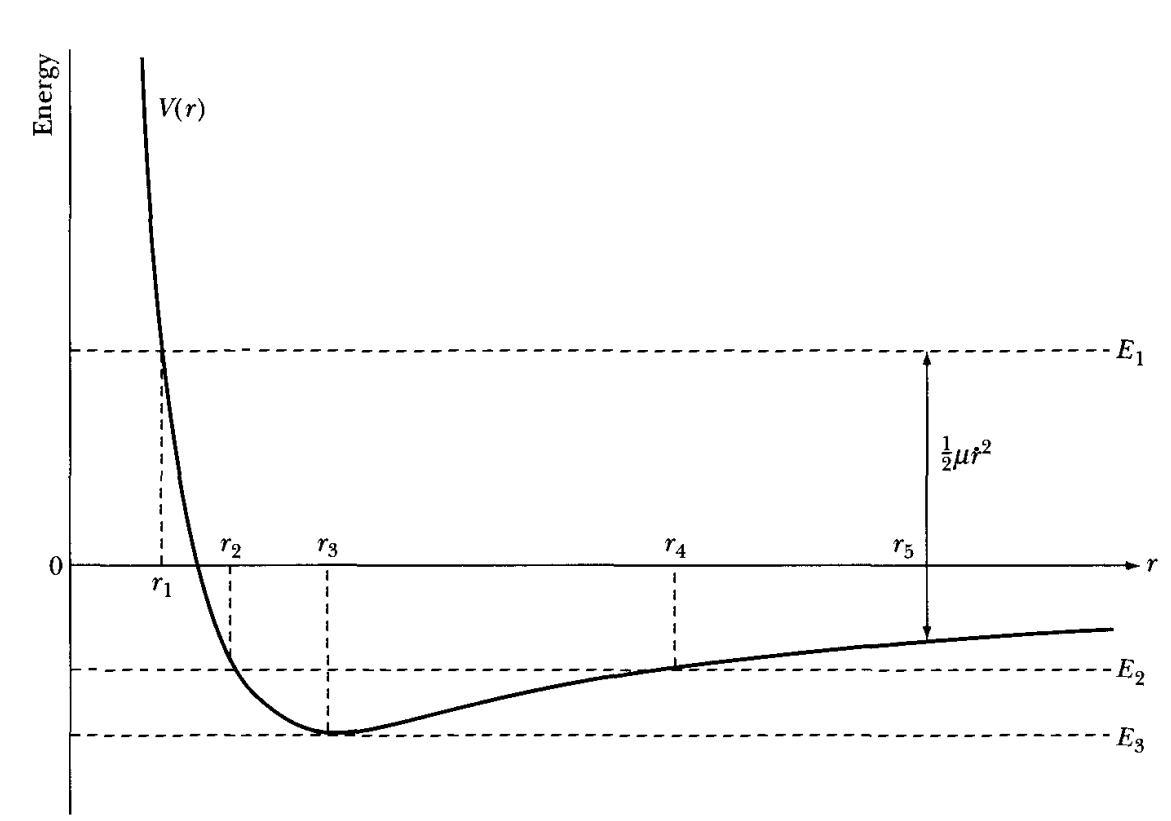
\includegraphics[scale=0.39]{PE.png}
\end{center}
For energy $E_1$, the particle's motion is unbounded. For energy $E_2$, the particle is bounded with $r_2 \leq r \leq r_4$. For energy $E_3$, the motion has $r= r_3$ and is circular. For kinetic energy given by $T= \frac{1}{2}\mu r^2$ and potential energy given by $V(r)$ which converges to $0$ as $r$ approaches infinity, if the total energy is negative, and if the total energy lies between zero and the minimum value of $V(r)$, as does $E_2$, then the motion is bounded, with $r_2 \leq r\leq r_4$, the values $r_2$ and $r_4$ are the turning points, or the apsidal distances, of the orbit. If $E$ equals the minimum value of the effective potential energy, as does $E_3$, then the radius of the particle's path is limited to the single value $r_3$, and then $\dot{r} = 0$ for all values of the time, hence the motion is circular. \\

The orbits of the various conic sections are shown together with their eccentricities $\epsilon$:
\begin{center}
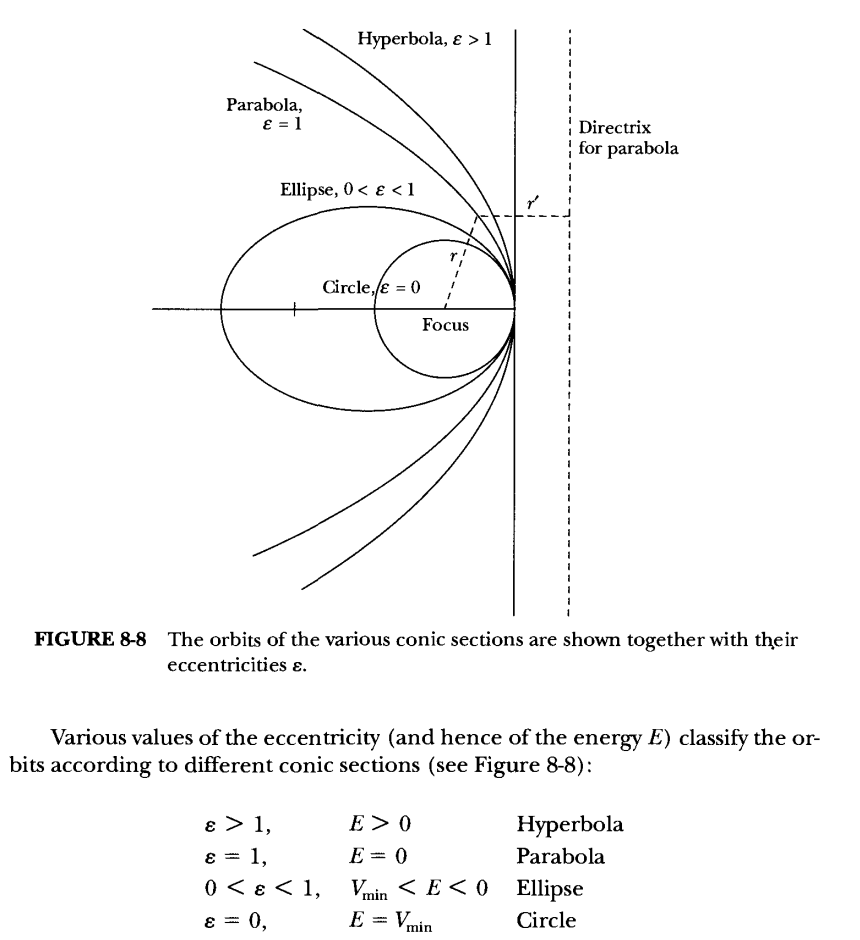
\includegraphics[scale=0.65]{epsilon.png}
\end{center}
\newpage
Kepler's First Law states the following for a two-body system with distance $r$ between the two bodies:
\begin{align*}
\frac{\alpha}{r} = 1+\epsilon \cos(\theta)
\end{align*}
The minimum value for $r$ occurs when $\theta = 0$ by assumption, or when $\cos(\theta)$ is at maximum. Here we can rewrite equation (T) as the following:
\begin{align*}
\theta(r) =  \int\frac{(l / r^2 )\, dr}{\sqrt{ 2\mu \left( E + \frac{k}{r} - \frac{l^2}{2\mu r^2} \right)}} + K
\end{align*}
where $K$ is a constant corresponds to measuring $\theta$ from $r_{min}$, which position is called the pericenter. The maximum value of $r$, $r_{max}$, on the other hand, is called the apocenter. The general term for turning points is apsides. The corresponding terms for motion about the Sun are perihelion and aphelion, and for motion about Earth, perigee and apogee. \\

\begin{center}
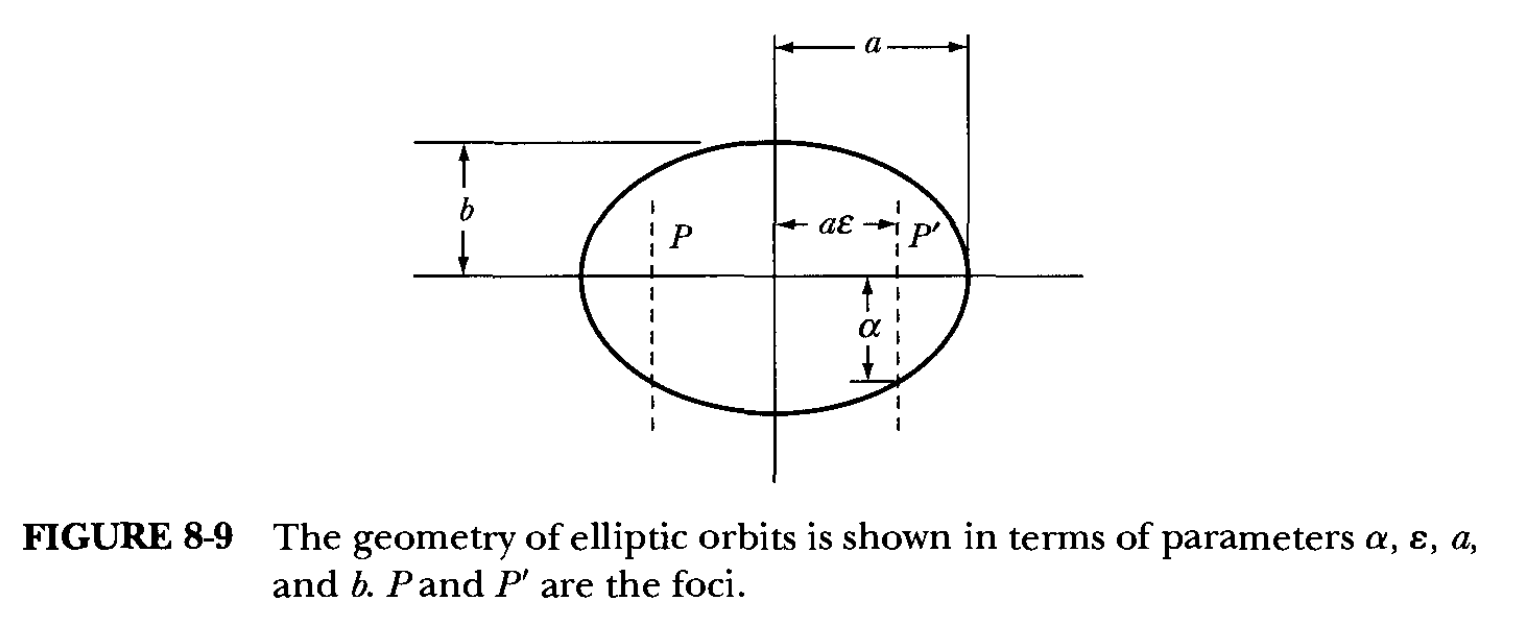
\includegraphics[scale=0.39]{ellipse.png}
\end{center}
With simple geometry, we get the following relations:
\begin{align*}
2a = r_{min}+r_{max} = \frac{\alpha}{1+\epsilon} + \frac{\alpha}{1-\epsilon} \qquad\Rightarrow\qquad \alpha = a(1+\epsilon)(1-\epsilon)
\end{align*}
\begin{align*}
r_{min}=\frac{a(1+\epsilon)(1-\epsilon)}{1+\epsilon}\qquad\qquad\qquad\qquad r_{max} = \frac{\alpha(1+\epsilon)(1-\epsilon)}{1-\epsilon}
\end{align*}
The ellipse has focal length $c = \epsilon a$, with $a^2 = b^2 + c^2 = b^2 + (\epsilon a)^2$, hence we can write the followings:
\begin{align*}
a = \frac{\alpha}{1-\epsilon^2} = \frac{l^2/(\mu k)}{-\frac{2El^2}{\mu k^2}} = \frac{k}{2|E|} \qquad \qquad\qquad b^2 = a^2(1-\epsilon^2) =\frac{\alpha^2}{1-\epsilon^2}= \frac{\alpha(a(1-\epsilon^2))}{(1-\epsilon^2)} = \alpha a
\end{align*}
Combining the results, we write:
\begin{align*}
a = \frac{\alpha}{1-\epsilon^2} = \frac{k}{2|E|}\qquad\qquad\qquad b=\sqrt{\alpha a} = \frac{\alpha}{\sqrt{1-\epsilon^2}} = \frac{l}{\sqrt{2\mu|E| }}
\end{align*}
\newpage
In the following we will now derive the Kepler's Second Law for Planetary motion:
\begin{center}
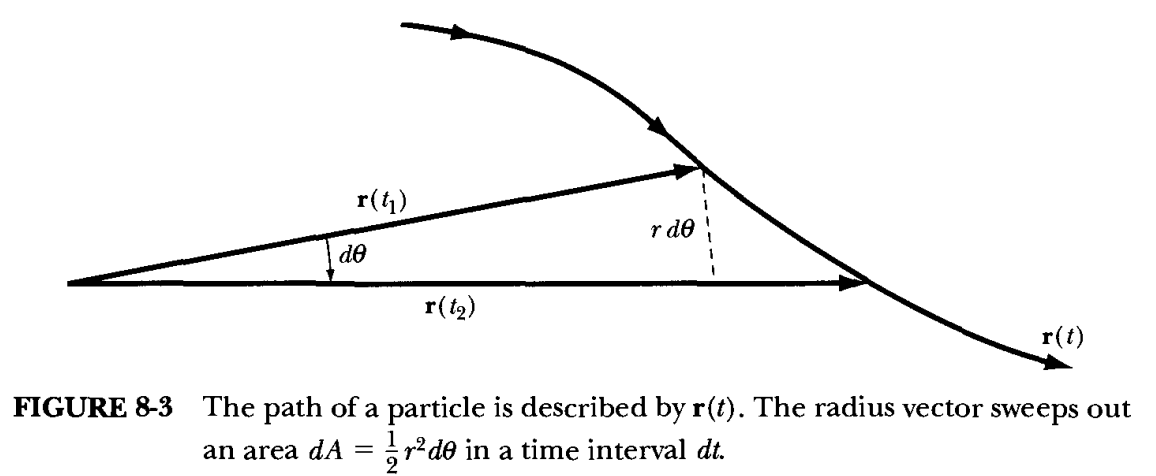
\includegraphics[scale=0.50]{K2L.png}
\end{center}
Rearranging we can write the following:
\begin{align*}
\frac{dA}{dt} = \frac{r^2}{2} \frac{d\theta}{dt} = \frac{r^2 \dot{\theta}}{2} = \frac{l}{2\mu} =\text{constant} \tag{11}
\end{align*}
Here equation (11) gives Kepler's Second Law. \\
\hfill\break\hfill\break
Finally, we will derive Kepler's Third Law for Planetary motion. Note that by Second Law we have the following, with $\tau$ denoting the period of one cycle:
\begin{align*}
\frac{dA}{dt} = \frac{l}{2\mu}\qquad \Rightarrow \qquad dt = \frac{2\mu}{l}\, dA \qquad \Rightarrow \qquad \tau = \frac{2\mu}{l}A
\end{align*}
Hence with results from above we get:
\begin{align*}
\tau = \frac{2\mu}{l}A=\frac{2\mu}{l}(\pi ab) = \frac{2\mu \pi}{l}\frac{k}{2|E|}\frac{l}{\sqrt{2\mu |E|}} = \pi k \sqrt{\frac{\mu}{2}}|E|^{-3/2}\tag{12}
\end{align*}
Equation (12) gives Kepler's Third Law. On the other hand, since we have $b = \sqrt{\alpha a}$, then we can write:
\begin{align*}
\tau = \frac{2\mu}{l}\pi a\sqrt{\alpha a} \qquad \Rightarrow \qquad \tau^2 = \left( \frac{2\mu}{l}\right)^2 \pi^2 a^3 \left( \frac{l^2}{\mu k}\right) = \frac{4\pi ^2}{k}\mu a^3 
\end{align*}
In the case where the two-bodies have masses $m_1$ and $m_2$ respectively, Kepler's Third Law under gravity can be formulated as the following:
\begin{align*}
\tau^2 = \frac{4\pi^2\left(\frac{m_1m_2}{m_1+m_2}\right)a^3}{Gm_1 m_2} = \frac{4\pi^2 a^3}{G(m_1+m_2)}
\end{align*}
in the case where $m_2  = M$ and $m_1 <<M$, we can write:
\begin{align*}
\tau^2 \approx \frac{4\pi^2 a^3}{GM}
\end{align*}
\newpage

\section[Orbital Dynamics]{\color{red} Orbital Dynamics \color{black}}
One can calculate the velocity changes need for a Holmann transfer by calculating the velocity of a spacecraft moving in the orbit of Earth around the Sun with radius $r_1$, and the velocity needed to kick it into an elliptical transfer orbit that can reach Mar's orbit, we are considering only the gravitational attraction of the Sun and not that of the Earth and Mars. 
\hfill\break

\begin{center}
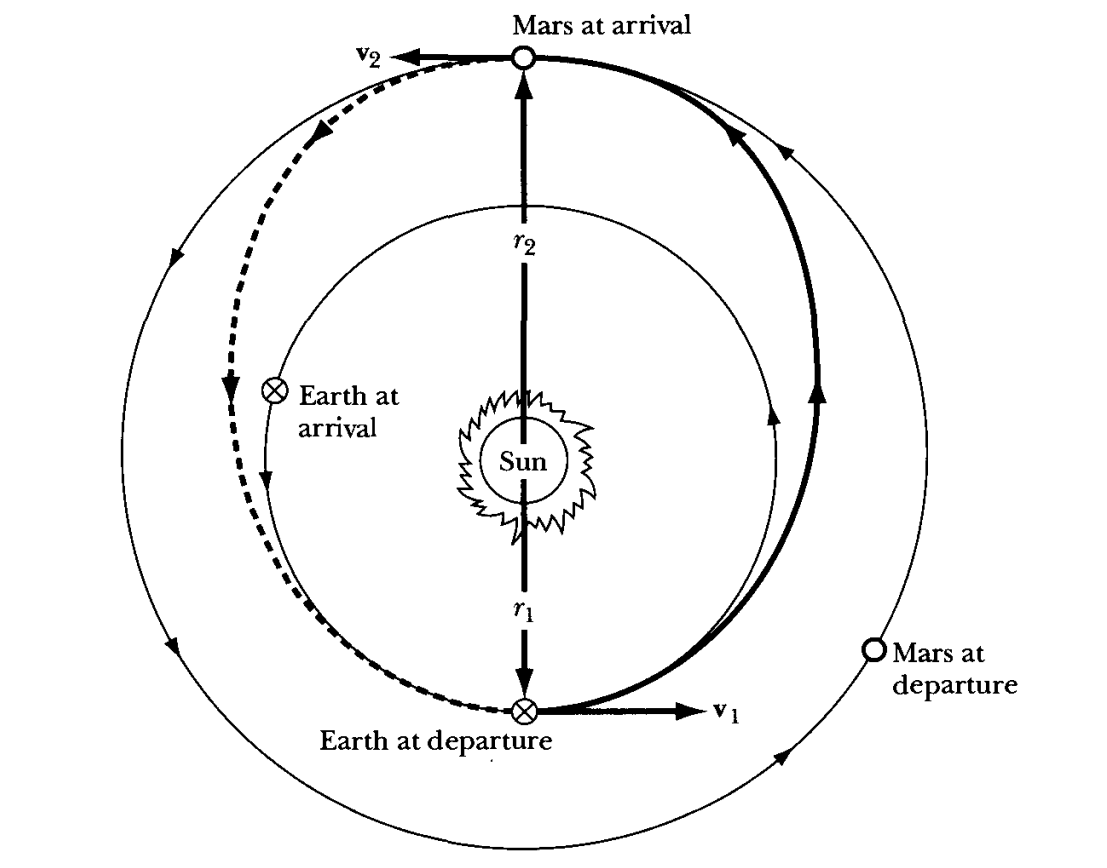
\includegraphics[scale=0.48]{OrbitalDynamics.png}\\
The Hohmann transfer for a round trip between Earth and Mars. \\
From a circular orbit to an elliptical orbit.
\end{center}
\hfill\break

For circles and ellipses we have:
\begin{align*}
E = -\frac{k}{2a}
\end{align*}
in our case, for a circular path around the Sun with radius $r_1$, we can write:
\begin{align*}
E = -\frac{k}{2r_1} = \frac{1}{2}mv_1^2 - \frac{k}{r_1}\qquad \Rightarrow \qquad v_1 = \sqrt{\frac{k}{mr_1}}
\end{align*}
and similarly with radius $r_2$, we get the following:
\begin{align*}
v_2 = \sqrt{\frac{k}{mr_2}}
\end{align*}
We here denote the semimajor axis of the transfer ellipse by $a_t$, then we get:
\begin{align*}
2a_t = r_1 +r_2
\end{align*}
We can calculate the energy at the perihelion for the transfer ellipse:
\begin{align*}
E_t = \frac{-k}{r_1 + r_2} = \frac{1}{2}mv_{t1}^2 - \frac{k}{r_1}
\end{align*}
where $v_{t1}$ is the perihelion transfer speed. Rearranging we get the following:
\begin{align*}
v_{t1} = \sqrt{\frac{2k}{mr_1}\left( \frac{r_2}{r_1 + r_2}\right)}
\end{align*}
here the direction of $v_{t1}$ is along the direction of $v_1$. \\
Hence the speed transfer $\Delta v_1$ needed is given by the following:
\begin{align*}
\Delta v_1 = v_{t1} - v_1
\end{align*}
Similarly, for the transfer from the ellipse to the circular orbit of radius $r_2$, $\Delta v_2 = v_2 - v_{t2}$, where $v_{t2}$ is given by the following:
\begin{align*}
v_{t2} = \sqrt{\frac{2k}{mr_2}\left( \frac{r_1}{r_1 + r_2}\right)}
\end{align*}
and we note that the direction of $v_{t2}$ is along the direction of $v_2$. \\

The total time required to make the transfer $T_t$ is a half-period of the transfer orbit:
\begin{align*}
T_t = \frac{\tau_t}{2} = \pi \sqrt{\frac{m}{k}} a_t^{3/2}
\end{align*}
where we have previously derived that $\tau$ is given by the following:
\begin{align*}
\tau^2 = \frac{4\pi^2}{k}\mu a^3 \qquad \Rightarrow \qquad \tau  = \sqrt{\frac{4\pi^2}{k}\mu a^3 }
\end{align*}

\newpage
\chapter{Dynamics of a System of Particles}
\section[Center of Mass Frame]{\color{red}Center of Mass Frame\color{black}}
Consider some particles, each with mass $m_{\alpha}$ at $\vec{r}_{\alpha}$, with $\alpha \in A$ and $A$ is an indexing set. \\
The total mass of the system is then given by he following:
\begin{align*}
M = \sum_{\alpha}m_{\alpha}
\end{align*}
and the center of mass position vector and velocity vector are given as:
\begin{align*}
\vec{R}_{CM} = \frac{1}{M}\sum_{\alpha}m_{\alpha} \vec{r}_{\alpha}\qquad\qquad\qquad \vec{V}_{CM} = \frac{1}{M}\sum_{\alpha}m_{\alpha}\vec{v}_{\alpha}
\end{align*}
The internal interaction force is zero by Newton's Third Law, then we can write the following if the external force on the system $\vec{F}_{ext} $ vanishes:
\begin{align*}
\vec{F}_{ext} = 0 \qquad \Rightarrow\qquad \vec{V}_{CM} = \text{constant} \qquad \Rightarrow \qquad \frac{1}{M}\sum_{\alpha}m_{\alpha}\vec{v}_{\alpha} = 0
\end{align*}

For a continuous distribution of mass $M$, one can find the center of mass position as the following:
\begin{align*}
\vec{R} = \frac{\int_M \vec{r}\, dm}{\int_M dm}
\end{align*}

In the center of mass frame, we can write the following:
\begin{align*}
\vec{F}_{ext} = M \frac{d\vec{V}_{CM}}{dt} = \frac{d(M\vec{V}_{CM})}{dt} = \frac{d\vec{P}_{CM}}{dt}
\end{align*}
Hence if we have $\vec{F}_{ext} = 0$, then $\vec{P}_{CM}$ is a constant, the total momentum conserves. In which case we can set the origin of the coordinate system as the position of the center of mass, so that we have the followings hold:
\begin{align*}
\vec{R}_{CM} = 0\qquad\qquad\qquad\qquad\qquad \sum_{\alpha}m_{\alpha}\vec{v}_{\alpha} = 0
\end{align*}
Now let $\vec{L}_{\alpha}$ denote the angular momentum of each of the particles, then we can write the total angular momentum of the system:
\begin{align*}
\vec{L} = \sum_{\alpha}\vec{L}_{\alpha} = \sum_{\alpha}(\vec{r}_{\alpha}\times \vec{p}_{\alpha}) &= \sum_{\alpha}(\vec{r}_{\alpha}\times m_{\alpha}\dot{\vec{r}}_{\alpha})\\
&= \sum_{\alpha}(\vec{r}_{\alpha}' + \vec{R}) \times m_{\alpha}(\dot{\vec{r}}_{\alpha}' + \dot{\vec{R}}) \\
&= \sum_{\alpha}m_{\alpha}\left( (\vec{r}_\alpha' \times \dot{\vec{r}}_{\alpha}') + (\vec{r}'_{\alpha}\times \dot{\vec{R}}) + (\vec{R}\times \dot{\vec{r}}_{\alpha}') + (\vec{R}\times \dot{\vec{R}})\right) \tag{*}
\end{align*}
where we define:
\begin{align*}
\vec{r}_{\alpha} = \vec{R}+\vec{r}'_{\alpha} \qquad\qquad\qquad L_{\alpha} = \vec{r}_{\alpha}\times \vec{p}_{\alpha}
\end{align*}

Here we note that:
\begin{align*}
\sum_{\alpha}m_{\alpha}\left(\vec{r}'_{\alpha}\times \dot{\vec{R}} + (\vec{R}\times \dot{\vec{r}}_{\alpha}'\right) = \left( \sum_{\alpha}m_{\alpha} \vec{r}'_{\alpha}\right) \times \dot{\vec{R}} + \vec{R}\times \frac{d}{dt}\left( \sum_{\alpha}m_{\alpha} \vec{r}'_{\alpha}\right) \tag{1}
\end{align*}
while we have:
\begin{align*}
\sum_{\alpha}m_{\alpha}\vec{r}'_{\alpha} = \sum_{\alpha}m_{\alpha}(\vec{r}_{\alpha} - \vec{R}) = \sum_{\alpha}m_{\alpha}\vec{r}_{\alpha} - \vec{R}\sum_{\alpha}m_{\alpha} = M\vec{R} = M\vec{R} = \vec{0}
\end{align*}
Hence concluding we see that equation (1) vanishes, and hence equation (*) becomes:
\begin{align*}
\vec{L} = M \vec{R}\times \dot{\vec{R}} + \sum_{\alpha}\vec{r}_{\alpha}' \times \vec{p}_{\alpha}' = \vec{R}\times \vec{P} + \sum_{\alpha}\vec{r}'_{\alpha} \times \vec{p}'_{\alpha}
\end{align*}
Here we see that the total angular momentum about an origin is the sum of the angular momentum of the center of mass about that origin and the angular momentum of the system about the position of the center of mass. Now let $\vec{F}_{\alpha}$ denote the external force on mass $m_\alpha$, and $\vec{f}_{\alpha\beta}$ denote the internal force on $m_\alpha$ exerted by $m_{\beta}$, then we can write the following:
\begin{align*}
\dot{\vec{L}}_{\alpha} = \vec{r}_{\alpha}\times \dot{\vec{p}}_{\alpha} = \vec{r}_{\alpha}\times \left( \vec{F}_{\alpha}+ \sum_{\beta}\vec{f}_{\alpha\beta}\right)
\end{align*}
Hence we can write:
\begin{align*}
\dot{\vec{L}} = \sum_{\alpha}\dot{\vec{L}}_{\alpha} 
&= \sum_{\alpha}\left(\vec{r}_{\alpha}\times \vec{F}_{\alpha}\right)+\sum_{\alpha,\ \beta \neq \alpha}\left(\vec{r}_{\alpha}\times \vec{f}_{\alpha\beta}\right) \\
&=\sum_{\alpha}\left(\vec{r}_{\alpha}\times \vec{F}_{\alpha}\right)+\sum_{\alpha< \beta}\left((\vec{r}_{\alpha}\times \vec{f}_{\alpha\beta}) + (\vec{r}_{\beta}\times \vec{f}_{\beta\alpha})\right)\\
&=  \sum_{\alpha}\left(\vec{r}_{\alpha}\times \vec{F}_{\alpha}\right)+0\\
&=\sum_{\alpha}\left(\vec{r}_{\alpha}\times \vec{F}_{\alpha}\right)\\
&\coloneqq \sum_{\alpha}\vec{N}_{\alpha} \\
&\coloneqq \vec{N}
\end{align*}
where $\vec{N}$ is the external torque on the system, and $\vec{N}_{\alpha}$ is the external torque on each of the mass $m_{\alpha}$. This shows that the if the net resultant external torques about a given axis vanish, then the total angular momentum of the system about that axis remains constant in time. \\

Now we will investigate the energy of the system, first note that we can write the following:
\begin{align*}
\dot{\vec{r}}_{\alpha} \cdot \dot{\vec{r}}_{\alpha} = v_{\alpha}^2 &= \left(\dot{\vec{r}}_{\alpha}' + \dot{\vec{R}}\right)\cdot \left(\dot{\vec{r}}_{\alpha}' + \dot{\vec{R}}\right)\\
&=\left(\dot{\vec{r}}_{\alpha}' \cdot \dot{\vec{r}}_{\alpha}'\right)+2\left(\dot{\vec{r}}_{\alpha}'\cdot \dot{\vec{R}}\right) + \left(\dot{\vec{R}}\cdot \dot{\vec{R}}\right)\\
&= \left(v'_{\alpha}\right)^2 + 2\left(\dot{\vec{r}}_{\alpha}' \cdot \dot{\vec{R}}\right)+ V^2 
\end{align*}
where $\vec{v}' = \dot{\vec{r}}'$ and $V$ is the speed of the center of mass. As computed previously, we know that we have: 
$$\frac{d}{dt}\left( \sum_{\alpha}m_{\alpha}\vec{r}_{\alpha}' \right)= 0$$
Hence we can write the following:
\begin{align*}
T = \sum_{\alpha}\frac{1}{2}m_{\alpha}v_{\alpha}^2 &= \sum_{\alpha}\frac{1}{2}m_{\alpha}(v'_{\alpha})^2 + \sum_{\alpha}\frac{1}{2}m_{\alpha}V^2 + \dot{\vec{R}}\cdot \left(\frac{d}{dt}\left( \sum_{\alpha}m_{\alpha}\vec{r}_{\alpha}' \right)\right) \\
&=\sum_{\alpha}\frac{1}{2}m_{\alpha}(v'_{\alpha})^2 + \sum_{\alpha}\frac{1}{2}m_{\alpha}V^2 
\end{align*}
Here we see that the total kinetic energy of the system is the sum of kinetic energy of a particle of mass $M$ moving with the velocity of the center of mass and kinetic energy of motion of the individual particles  relative to the center of mass. Here we also note that the total energy for a conservative system is constant.\\
\newpage

\section[Collision of Two Particles]{\color{red}Collision of Two Particles\color{black}}
Now suppose we have two particles, with masses $m_1$ and $m_2$, initially they have speed $u_1$ and $u_2$ respectively, then they collide, and after the collision, they have speed $v_1$ and $v_2$ respectively. By energy conservation, assume there is no change in potential energy for the two particles in this process, or one might assume that the collision happens in infinitesimal time, we can write:
\begin{align*}
Q + \frac{1}{2}m_1u_1^2 + \frac{1}{2}m_2 v_2^2 = \frac{1}{2}m_1v_1^2 + \frac{1}{2}m_2v_2^2
\end{align*}
where $Q$ is called the $Q$-value and represents the energy loss or gain in the collision. \\
If we have $Q = 0$, the collision is said to be elastic, and kinetic energy during the collision conserves.\\ If $Q>0$, the collision is said to be exoergic, and kinetic energy is gained during the collision. \\If $Q<0$, the collision is said to be endoergic, kinetic energy is lost during the collision. \\




Now consider a collision occurs between two particles, one of which is moving and one of which is at rest. The actual measurements are made in the laboratory coordinate system in which the observer is at rest. In the laboratory coordinate system, one of the particles is normally moving, and the the struck particle is normally at rest. It is indeed simpler to describe the effects of the collision in a  coordinate system in which the center the center of mass of the two particles is at rest, in which coordinate system both particles are moving. Here we refer to these two coordinate systems simply as the CM and the LAB systems. \\

Let $m_1$ be the mass of the moving particles, and let $m_2$ be the mass of the struck particle. The struck particle is initially at rest.\\

For the moving particle of mass $m_1$, let $\vec{u}_1$ and $\vec{v}_1$ be the initial and final velocities, respectively, of the particle in the LAB frame. Let $\vec{u}'$ and $\vec{v}_1'$ be the initial and final velocities, respectively, of the particle in the CM system. We define similarly for $\vec{u}_2$, $\vec{v}_2$, $\vec{u}_2'$, and $\vec{v}_2'$ for the struck particle $m_2$. Here we note that $\vec{u}_2 = 0$. \\

Let $\vec{V}$ be the velocity of the center of mass of the two particles in the LAB frame. Let $\psi$ be the angle through which $m_1$ is deflected in the LAB frame. Let $\zeta$ be the angle through which $m_2$ is deflected in the LAB frame. Let $\theta$ be the angle through which $m_1$ and $m_2$ are deflected int he CM frame. Let $T_0$ be the total initial kinetic energy in the LAB frame, and let $T_0'$ be the total initial kinetic energy in the CM frame. Let $T_1$ be the final kinetic energy of $m_1$ in the LAB frame, and let $T'_1$ be the final kinetic energy of $m_1$ in the CM frame. Define $T_2$ and $T_2'$ similarly. \\

We assume throughout that the scattering is axially symmetric so that no azimuthal angle is needed to be introduced. However, axial symmetry is not always found in scattering problems, which is particularly true in certain quantum mechanical systems. We will focus on the situation where elastic collision takes place, that is, both kinetic energy and momentum of the system conserves.\\

\begin{center}
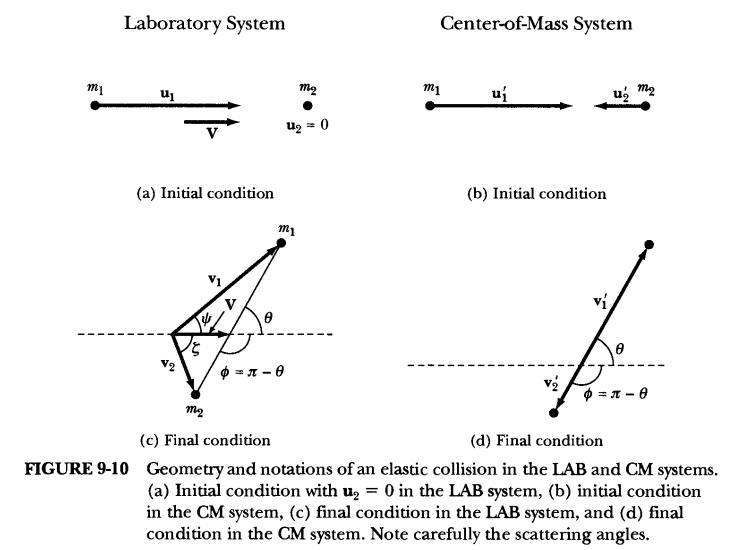
\includegraphics[scale=0.69]{scatter.png}
\end{center}

If $V<v_1'$, then only one possible relation exists between $\vec{V}$, $\vec{v}_1$, $\vec{v}_1$, and $\theta$. But if $V>v_1'$, then for every set $V, v_1'$, there exists two possible scattering angles and laboratory velocities, $v_{1,b}$, $\theta_b$ and $v_{1,f},\theta_f$, where the designations $b$ and $f$ stand for backward and forward.\\

\begin{center}
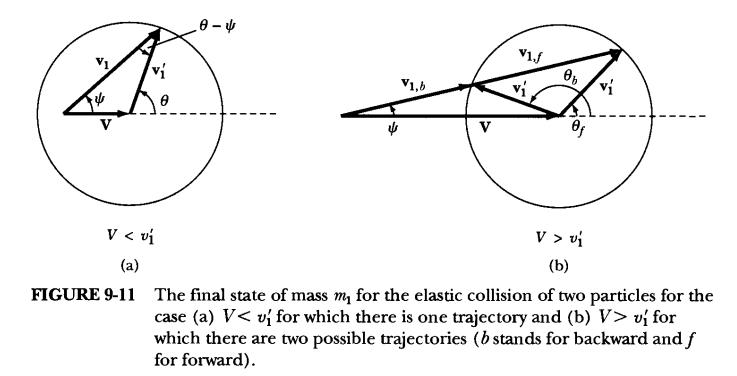
\includegraphics[scale=0.69]{scatterf&b.png}
\end{center}

Here we let $\vec{r}_1$ and $\vec{r}_2$ denote the position of particle $m_1$ and $m_2$, respectively, let $\vec{R}$ denote the position of the center of mass. By the definition of the center of mass frame, and results derived previously, we have the followings:
\begin{align*}
m_1\vec{r}_1 + m_2 \vec{r}_2 = M\vec{R} \qquad\qquad\qquad\qquad m_1\vec{u}_1 + m_2 \vec{u}_2 = M\vec{V}
\end{align*}
Here we note that $\vec{u}_2 = 0$, and we define $M= m_1 + m_2$, then rearranging we get the following:
\begin{align*}
\vec{V} = \frac{m_1 \vec{u}_1}{m_1+m_2}
\end{align*}
By the same reasoning, since $m_2$ is initially at rest in the LAB frame, then in the CM frame, $m_2$ has same speed as $V$, but in opposite direction:
\begin{align*}
\vec{u}_2' = -\vec{V} = -\frac{m_1\vec{u}_1}{m_1+m_2}\qquad \Rightarrow \qquad u_2' = \frac{m_1 u_1}{m_1 + m_2}
\end{align*}
The total linear momentum in CM frame is zero, and hence before the collision, the particles move directly toward each other, and after the collision they move in exactly opposite directions. Here we assume that the collision is elastic and hence by conservation of energy and momentum, we obtain the following relationship:
\begin{align*}
u_1' = v_1' \qquad\qquad\qquad\qquad\qquad u_2' = v_2'
\end{align*}
Here $u_1$ is the relative speed of the two particles in the CM or the LAB frame. $u_1 = u_1 + u_2 = u_1' + u_2'$. Hence we can write the following:
\begin{align*}
v_2' = u_2' = 
\frac{m_1 u_1}{m_1 + m_2}
\qquad\qquad\qquad\qquad\qquad 
v_1' = u_1' = u_1 - u_2' =
\frac{m_2 u_1}{m_1 + m_2}
\end{align*}
By geometry from Figure 9-11, we have the following:
\begin{align*}
v_1' \sin(\theta) = v_1 \sin(\psi)\qquad\qquad\qquad\qquad\qquad v_1' \cos(\theta) +V = v_1 \cos(\psi)
\end{align*}
Combining we get the following:
\begin{align*}
\tan(\psi) = \frac{v_1' \sin(\theta)}{v_1' \cos(\theta) +V} = \frac{\sin(\theta)}{\cos(\theta) +(V/v_1')}
\end{align*}
From the above we can compute:
\begin{align*}
\frac{V}{v_1'} = \frac{m_1 u_1/(m_1+m_2)}{m_2 u_1 /(m_1 +m_2)} = \frac{m_1}{m_2} \tag{R}
\end{align*}
Note here the ratio given by equation (R) governs the scattering process indicated on Figure 9-11 (a) and (b). Combining we get the following:
\begin{align*}
\tan(\psi) = \frac{\sin(\theta)}{\cos(\theta) + (m_1/m_2)}
\end{align*}
we see that if $m_1 << m_2$, the LAB and CM scattering angles are approximately equal, that is, the particle $m_2$ is but little affected by the collision with $m_1$ and acts essentially as a fixed scattering center.\\

If we have $m_1 = m_2$, then we have the following instead:
\begin{align*}
\psi = \frac{\theta}{2} \qquad \qquad \qquad \qquad\qquad \text{if }m_1 = m_2
\end{align*}
Since the maximum value of $\theta$ is $180^\circ$. Then for $m_1 = m_2$ there can be no scattering in the LAB system at angles greater than $90^\circ$. \\

For the particle at rest, we obtain the following graph:
\begin{center}
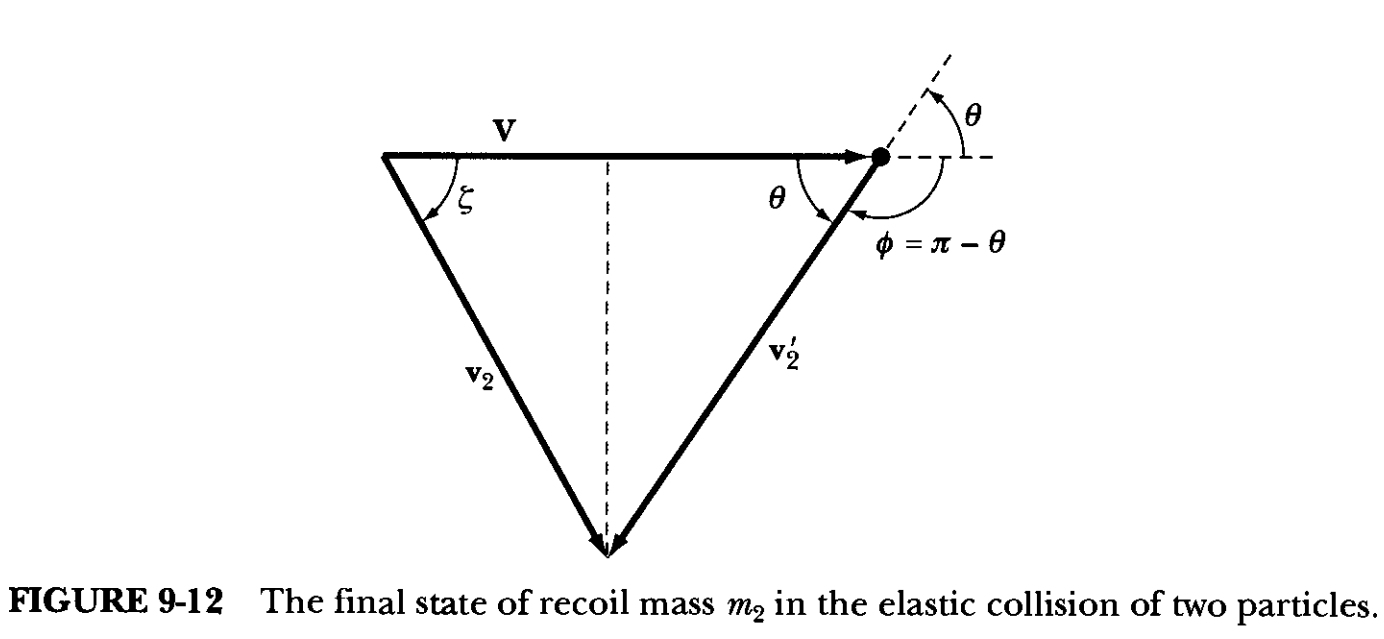
\includegraphics[scale=0.35]{restParticle.png}
\end{center}
Hence by simple geometry, we can write the following:
\begin{align*}
v_2 \sin(\zeta) = v_2' \sin(\theta) \qquad\qquad\qquad\qquad\qquad v_2 \cos(\zeta) = V- v_2' \cos(\theta)
\end{align*}
Combining we get the following:
\begin{align*}
\tan(\zeta) = \frac{v_2'\sin(\theta)}{V- v_2' \cos(\theta)} = \frac{\sin(\theta)}{(V/v_2')-\cos(\theta)}
\end{align*}
By results from above, we know that $v_2' = u_2' = V$, hence we can write:
\begin{align*}
\tan(\zeta) = \frac{\sin(\theta)}{1 - \cos(\theta)} = \cot\left( \frac{\theta}{2}\right) = \tan\left( \frac{\pi}{2} - \frac{\theta}{2}\right)
\end{align*}
Thus we have:
\begin{align*}
2\zeta = \pi - \theta \coloneqq \phi
\end{align*}
For particles with equal mass $m_1 = m_2$, we have $\theta = 2\psi$, combining we get:
\begin{align*}
\zeta + \psi = \frac{\pi}{2} \qquad\qquad\qquad \text{if }m_1 = m_2
\end{align*}
Hence the scattering of particles of equal mass always produces a final state in which the velocity vectors of the particles are at right angles if one of the particle is initially at rest. Note that this results is only valid in the nonrelativistic limit.\\

\subsection*{Kinematics of Elastic Collisions}
Using the settings from above, we have the following:
\begin{align*}
T_0 = \frac{m_1 u_1^2}{2} \qquad \qquad \qquad T_{0}' = \frac{m_1 (u'_1)^2 + m_2 (u'_2)^2}{2}
\end{align*}
and from results derived above, we get the following:
\begin{align*}
T_0' = \frac{1}{2}\frac{m_1m_2u_1^2}{m_1 + m_2}  = \frac{m_2 }{m_1 + m_2} \, T_0
\end{align*}
which indicates that the initial kinetic energy in the CM system $T_0'$ is always a fraction $\frac{m_2}{m_1+m_2}<1$ of the initial LAB energy. For the final energy in the CM frame, we get the following:
$$
T_1' = \frac{m_1(v_1')^2}{2} = \frac{m_1u_1^2}{2}\left( \frac{m_2}{m_1+m_2}\right)^2  = \left( \frac{m_2}{m_1+m_2}\right)^2 T_0 
$$
$$
T_2' = \frac{m_2(v_2')^2}{2} = \frac{m_2u_1^2}{2}\left( \frac{m_1}{m_1 + m_2}\right)^2 = \frac{m_1m_2}{(m_1 + m_2)^2}T_0
$$
To obtain $T_1$ in terms of $T_0$, we use Law of Cosine and write the following:
\begin{align*}
\frac{T_1}{T_0} = \frac{m_1 v_1^2}{m_1 u_1^2} = \frac{v_1^2}{u_1^2} = \frac{(v_1')^2}{u_1^2}- \frac{V^2}{u_1^2} + \frac{2v_1V\cos(\psi)}{u_1^2}
\end{align*}
From the results above, we get the following:
\begin{align*}
\frac{v_1'}{u_1} = \frac{m_2}{m_1 + m_2} \qquad\qquad \frac{V}{u_1} = \frac{m_1}{m_1 + m_2} \qquad\qquad \frac{2v_1 V}{u_1^2}\cos(\psi) = 2\left( v_1' \frac{\sin(\theta)}{\sin(\psi)}\right) \frac{V \cos(\psi)}{u_1^2}
\end{align*} 
and we have:
\begin{align*}
\frac{\sin(\theta)\cos(\psi)}{\sin(\psi)} = \frac{\sin(\theta)}{\tan(\psi)} = \cos(\theta) + \frac{m_1}{m_2}
\end{align*}
Now combining we get the following:
\begin{align*}
\frac{T_1}{T_0} = \left(\frac{m_2}{m_1 + m_2} \right)^2 - \left( \frac{m_1}{m_1+m_2}\right)^2 + \frac{2m_1m_2}{(m_1+m_2)^2}\left( \cos(\theta) + \frac{m_1}{m_2}\right) = 1-\frac{2m_1m_2(1-\cos(\theta))}{(m_1+m_2)^2}
\end{align*}
Similarly, we obtain the following in terms of LAB scattering angle $\psi$:
\begin{align*}
\frac{T_1}{T_0} = \frac{m_1^2}{(m_1+m_2)^2} \left( \cos(\psi) \pm \sqrt{\left(\frac{m_2}{m_1}\right)^2 - \sin^2(\psi)}\right)^2 \tag{*}
\end{align*}
Here in equation (*), we take plus sign for the radical unless $m_1>m_2$. If $m_1 > m_2$, then the result is double-valued, and the following specifies the maximum value allowed for $\psi$:
\begin{align*}
\psi_{max} = \sin^{-1}\left(\frac{v_1'}{V} \right)=\sin^{-1}\left(\frac{m_2}{m_1} \right)
\end{align*}
The LAB energy of particle $m_2$ can be calculated from here:
\begin{align*}
\frac{T_2}{T_0} = 1- \frac{T_1}{T_0} = \frac{4m_1m_2\cos^2(\zeta)}{(m_1+m_2)^2} \qquad\qquad\qquad \text{if }\zeta \leq \frac{\pi}{2}
\end{align*}
Rearranging we get several further relationships:
\begin{align*}
\sin(\zeta) = \sqrt{\frac{m_1T_1}{m_2T_2}} \sin(\psi) \qquad\qquad \tan(\psi) = \frac{\sin(2\zeta)}{(m_1/m_2) -\cos(2\zeta)}\qquad\qquad \tan(\psi) = \frac{\sin(\phi)}{(m_1/m_2) - \cos(\phi)}
\end{align*}

If we have $m_2 = m _2$, we get the followings:
\begin{align*}
\frac{T_1}{T_0} = \cos^2 (\psi) \qquad\qquad \qquad\qquad \frac{T_2}{T_0} = \sin^2(\psi) \qquad\qquad\qquad\qquad\qquad \text{if }m_1= m_2
\end{align*}

\note In this section, only kinematic relationships are involved. We assumed the process to the elastic and non-relativistic. No attempt is made to predict a scattering angle or a final velocity, only equations connecting these quantities are obtained.\\


The center of mass of a system moves as if it were a single particle of mass equal to the total mass of the system, acted on by the total external force, and independent of the nature of the internal force, as long as they follow the weak form of Newton's Third Law. Hence the linear total momentum of the system is given by the following, with $\alpha$ being particles in the system:
\begin{align*}
\vec{P} = \sum_\alpha m_\alpha \dot{\vec{r}}_\alpha = \frac{d}{dt}\sum_\alpha m_\alpha \vec{r}_\alpha = \frac{d}{dt} (M\vec{R}) = M\dot{\vec{r}}\qquad\qquad\qquad\qquad \dot{\vec{P}} = M\ddot{\vec{R}} = \vec{F}
\end{align*}
where $\vec{F}$ is the external force experienced by the system. Thus the total linear momentum of the system is conserved if there is no external force.\\

The linear momentum of the system is the same as if a single particle of mass $M$ weer located at the position of the center of mass moving in the manner of the center of mass moves.\\

The total linear momentum for a system free of external forces is constant and equal to the linear momentum of the center of mass. 

\newpage
\section[Particle Scattering Cross Sections]{\color{red}Particle Scattering Cross Sections\color{black}}
In the following, we consider a situation when a repulsive force exists between $m_1$ and $m_2$. The particle $m_1$ approaches the vicinity of $m_2$ in such a way that if there were no force acting between the particles, $m_1$ would pass $m_2$, with a distance of closest approach $b$. The quantity $b$ is called the impact parameter. 
\begin{center}
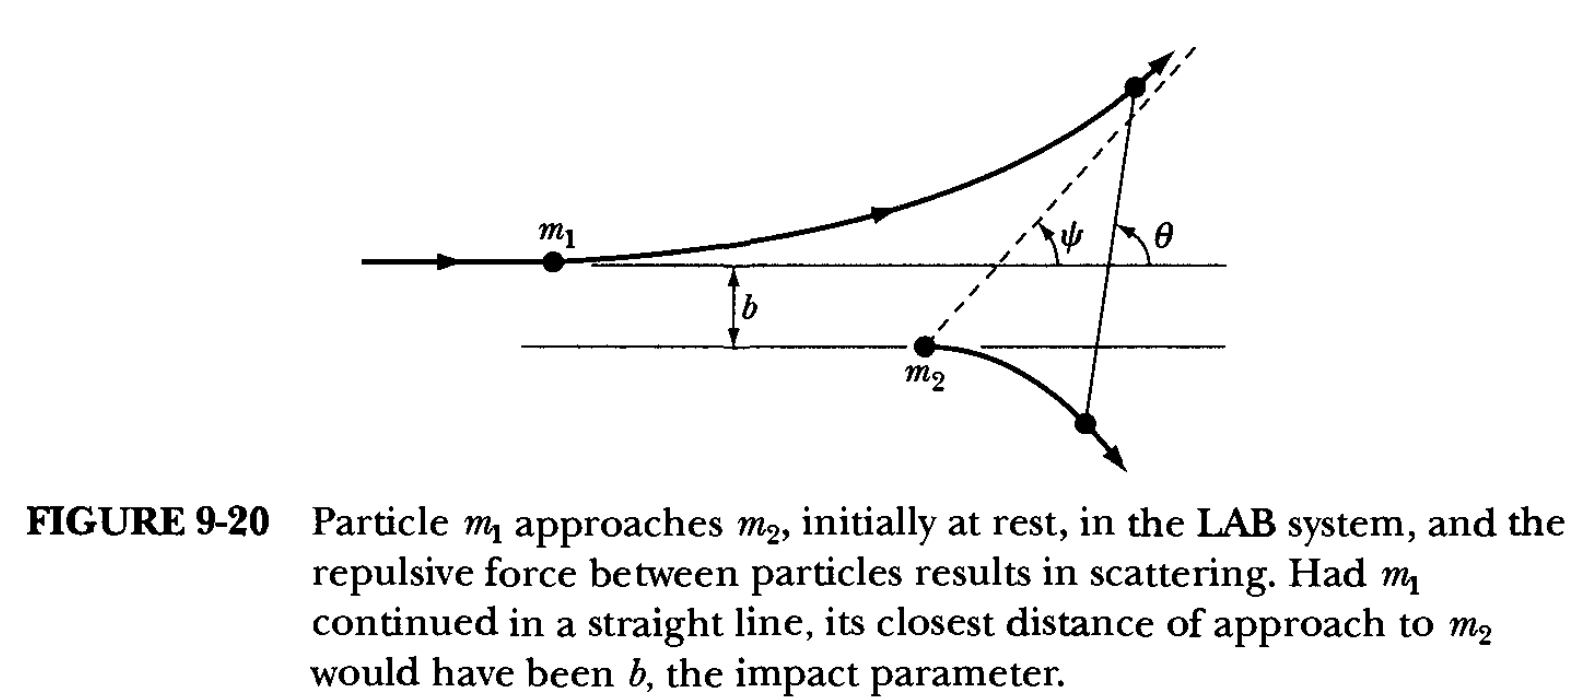
\includegraphics[scale=0.38]{scatter2.png}\\
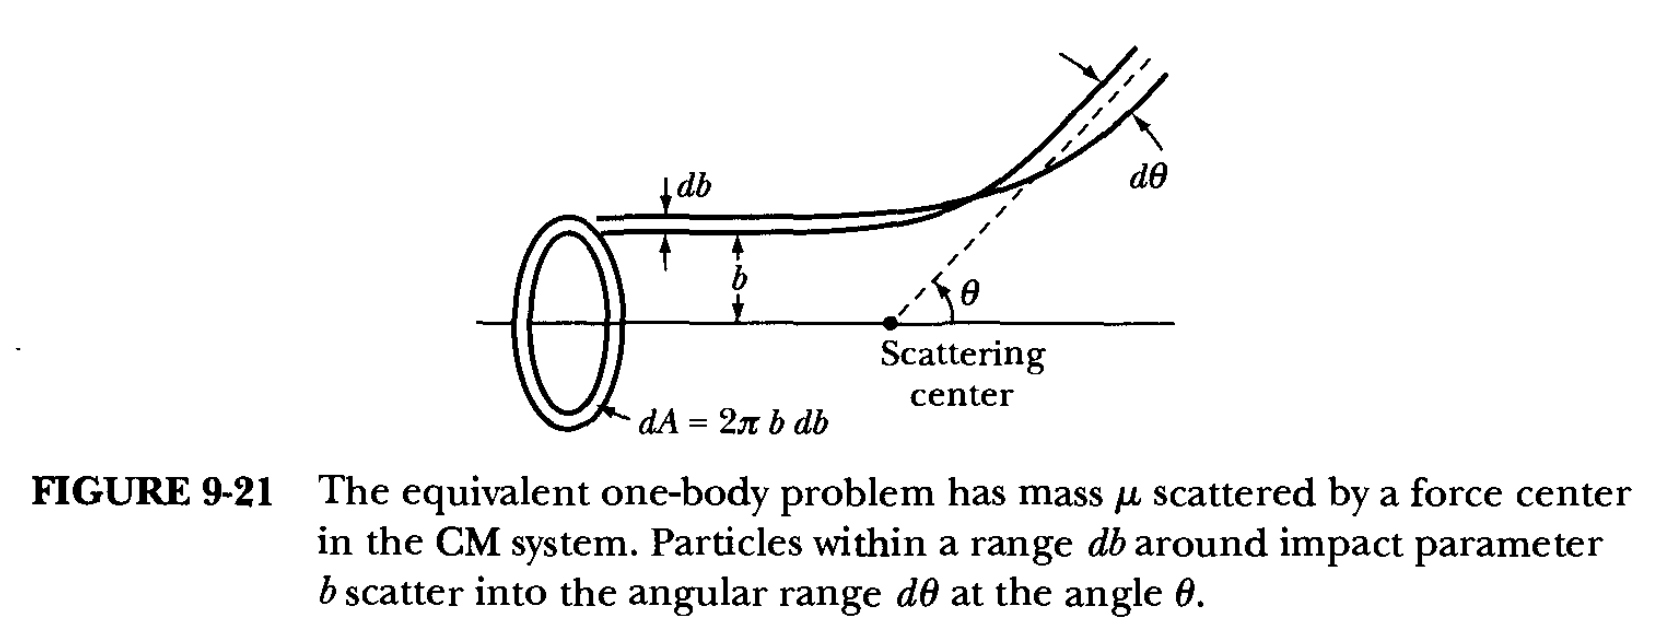
\includegraphics[scale=0.38]{scatter1.png}
\end{center}
From simple geometry of solid angle, we obtain the following graph:
\begin{center}
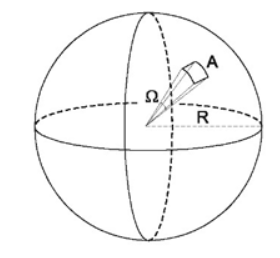
\includegraphics[scale=0.75]{solidAngle.png}
\end{center}
Here we have:
\begin{align*}
dA = (r\,d\theta)(r\sin(\theta)\, d\phi) = r^2 \sin(\theta) \,d\theta\, d\phi \qquad\qquad\qquad  d\Omega \coloneqq \frac{dA}{r^2} = \sin(\theta) \,d\theta\, d\phi
\end{align*}
As illustrated in Figure 9-21, if we view the beam of particle as shoot along the $z$-axis, force center at origin, the scattered particles will distributed around $z$ with $\phi$-symmetry. So by integrating $\phi$ in $[0,2\pi]$, we obtain the solid angle for such beam in theory in the following form:
\begin{align*}
d\Omega' = 2\pi \sin(\theta) \,d\theta
\end{align*}
Hence, as illustrated in Figure 9-21, every  beam of particle in the annulus defined by $b$ and the $b+|db|$ area is scattered into the solid angle $d\Omega'$, define by $\theta$ and $\theta+d\theta$. \\

The beam intensity $n_b$ is defined as number of particle per unit area. Let $N$ denote the number of scattered particles, we obtain the equation of the scattering:
\begin{align*}
n_b 2\pi b |db| = \left(\frac{dN}{d\Omega'} \right)\, d\Omega' = \left( \frac{dN}{d\Omega'}\right) (2\pi \sin(\theta) d\theta)
\end{align*}
Here we define the differential cross-section:
\begin{align*}
\frac{d\sigma}{d\Omega'} \coloneqq \frac{1}{n_b}\frac{dN}{d\Omega'}
\end{align*}
Rearranging we get the following:
\begin{align*}
b|db| = \frac{1}{n_b} \frac{dN}{d\Omega'} \sin(\theta)\,d\theta = \frac{d\sigma}{d\Omega'} (\sin(\theta) \, d\theta)
\end{align*}
Now we define:
\begin{align*}
\sigma(\theta) \coloneqq \frac{d\sigma}{d\Omega'}  = \frac{b}{\sin(\theta)}\left| \frac{db}{d\theta}\right|
\end{align*}
Note here $|\frac{db}{d\theta}|$ is absolute. Positive $db$ may give negative $d\theta$, that is, increase in $b$ might result in decrease in $\theta$ as force become weaker and so we have less scattering. \\

In experiment, we often put our detector in a place with a distance $d$ from the interaction point, and the detector detects a total area $S$, so the solid angle coverage of the detector is given by:
\begin{align*}
\Delta \Omega = \frac{S}{d^2}
\end{align*}

Now we can calculate the cross section $\sigma(\theta)$ if the force law for scattering is given, and we can use $\sigma(\theta)$ to predict the event rate in experiment set up:
\begin{align*}
\sigma(\theta) = \frac{1}{n_b}\frac{dN}{d\Omega'}\qquad \Rightarrow \qquad N(\theta) = n_b\cdot \sigma(\theta)\cdot \Delta \Omega
\end{align*}

\subsection*{Rutherford Scattering}
The force experienced by the $\alpha$ particle is given by:
\begin{align*}
F(r) = \frac{k}{r^2}
\end{align*}
In this problem, we have $E = T_0' = \frac{1}{2}m_1 v_0^2$, where $m_1$ is the mass of the $\alpha$ particle, and $v_0$ is the initial speed of the $\alpha$ particle. For impact parameter $b$, since angular momentum conserves, and $b$ gives the distance of closest approach, then we can write:
\begin{align*}
l = m_1 v_0 b
\end{align*}
Given, $E$ and $l$, we now have:
\begin{align*}
\alpha = \frac{l^2}{mk}\qquad\qquad\qquad \epsilon = \sqrt{1+ \left(\frac{2bT_0'}{k} \right)^2}
\end{align*}
The orbit of $\alpha$ particle is a hyperbola, which is symmetric about the line connecting the force center and point $A$, hence we have $\alpha = \beta  \coloneqq \Psi$. 
The orbit equation gives:
\begin{align*}
\frac{\alpha}{r} = 1+ \epsilon \cos(-\Psi) = 1+ \epsilon\cos(\Psi) 
\end{align*}
here we see that when $r \to \infty$, we have $\cos(\Psi) = -\frac{1}{\epsilon}$, then we can write:
\begin{align*}
\theta = \pi - 2\Psi \qquad\Rightarrow \qquad \Psi=\frac{\pi}{2} \qquad \Rightarrow \qquad \cos(\Psi) = \sin\left(-\frac{\theta}{2}\right) = -\frac{1}{\epsilon}
\end{align*}
Rearranging we get:
\begin{align*}
\sin\left(\frac{\theta}{2} \right) = \frac{1}{\epsilon} = \frac{1}{\sqrt{1+ \left(\frac{2bT_0'}{k} \right)^2}} \qquad \Rightarrow \qquad b=\frac{k}{2T'_0} \left( \frac{\cos(\theta/2)}{\sin(\theta/2)}\right)
\end{align*}
Hence we have:
\begin{align*}
\frac{db}{d\theta} = -\frac{k}{4T'_0}\frac{1}{\sin^2(\theta/2)}
\end{align*}
Now combining we get:
\begin{align*}
\sigma(\theta) = \frac{b}{\sin(\theta)}\left| \frac{db}{d\theta}\right| = \frac{b}{2 \sin(\theta/2)\cos(\theta/2)} \frac{k}{4T'_0\sin^2(\theta/2)} = \left(\frac{k}{4T_0'} \right)^2 \frac{1}{\sin^4(\theta/2)}
\end{align*}
\newpage
Since the total number of particles scattered into a unit solid angle must be the same in the LAB system as in the CM system. Then we must have:
\begin{align*}
\sigma(\theta)\, d\Omega'& = \sigma(\psi)\, d\Omega\\
\sigma(\theta) \cdot 2\pi \sin(\theta)\, d\theta &= \sigma(\psi) \cdot 2\pi \sin(\Psi) \, d\psi
\end{align*}
where $\theta$ and $\psi$ represent the same scattering angle but measured in the CM and LAB system, respectively, $d\Omega'$ and $d\Omega$ represent the same element of solid angle but measured in the CM and LAB frame, respectively, and $\sigma(\theta)$ and $\sigma(\psi)$ are the differential cross sections for the scattering in the CM and LAB frames, respectively. Thus we can write:
\begin{align*}
\sigma(\psi) = \sigma(\theta) \cdot \frac{\sin(\theta)}{\sin(\psi)}\frac{d\theta}{d\psi}
\end{align*}
Note here we have, from Figure 9-11 (a), and equations derived above:
\begin{align*}
\frac{\sin(\theta-\psi)}{\sin(\psi)} = \frac{m_1}{m_2} \tag{*}
\end{align*} 
Here we denote $\frac{m_1}{m_2} \coloneqq x$. Then we have:
\begin{align*}
0 = dx = \frac{\partial x}{\partial \psi}\,d\psi + \frac{\partial x}{\partial \theta}\, d\theta
\end{align*}
Rearranging we get:
\begin{align*}
\frac{d\theta}{d\psi} = \frac{\sin(\theta - \psi) \cos(\psi)}{\cos(\theta - \psi) \sin(\psi)} + 1 = \frac{\sin(\theta)}{\cos(\theta-\psi) \sin(\psi)}
\end{align*}
On the other hand, equation (*) also gives the following:
\begin{align*}
\frac{\sin(\theta - \psi) \cos(\psi)}{\sin(\psi)}+ \cos(\theta - \psi) = x\cos(\psi) + \cos(\theta - \psi)
\end{align*}
rearranging we get:
\begin{align*}
\frac{\sin(\theta)}{\sin(\psi)} = x\cos(\psi) + \cos(\theta - \psi) \qquad \qquad \qquad \cos(\theta - \psi) = \sqrt{1-x^2 \sin^2(\psi)}
\end{align*}
Combining all we get the following:
\begin{align*}
\sigma(\psi) = \sigma(\theta) \cdot \frac{\left( x\cos(\psi) + \sqrt{1-x^2 \sin^2 \psi}\right)^2}{\sqrt{1-x^2 \sin^2 \psi}}
\end{align*}
Equation (*) also suggests that we have:
\begin{align*}
\theta = \sin^{-1}(x\sin(\psi)) + \psi
\end{align*}
Here we got equations for cross section entirely in terms of angle $\psi$. The transformation assumes a simple form for a few cases. For $x = m_1/x_2 = 1$, we have $\theta = 2\psi$ by previous discussion, then we can write:
\begin{align*}
\sigma(\psi) = \left.\sigma(\theta)\right|_{\theta = 2\psi} \cdot 4\cos(\psi) \qquad \qquad \text{if }m_1 = m_2
\end{align*}
For $m_1 << m_2$, we have $x = 0$ and $\theta \approx \psi$, so we can write:
\begin{align*}
\sigma(\psi) =\left. \sigma(\theta) \right|_{\theta = \psi}\qquad \qquad \text{if }m_1 << m_2
\end{align*}
For $m_1 >> m_2$, the motion of $m_1$ will not be changed significantly, hence $\psi$ is small, so we have:
\begin{align*}
\frac{\sin(\theta-\psi)}{\sin(\psi)} = \frac{m_1}{m_2} \qquad \Rightarrow \qquad \sin(\theta) \approx \frac{m_1}{m_2}\,\psi
\qquad \qquad \text{if }m_1 >> m_2
\end{align*}


\newpage
\chapter{Dynamics of Rigid Bodies}

We define a rigid body as a collection of particles whose relative distances are constrained to remain absolutely fixed. In general, we need to have $6$ parameters to describe a rigid body motion, $3$ for center of mass translational motion, and $3$ for rotational motion.\\

\section[Rotation of a Rigid Body]{\color{red}Rotation of a Rigid Body\color{black}}
Consider a multiple particle rigid body $\{\text{partiacle }i \text{ of mass }m_i \text{ at position }\vec{r}_i\}$, rotates around an axis defined by $\vec{\omega}$. Here $\vec{r}_i$ is measured with respect to the origin $O$. 
\begin{center}
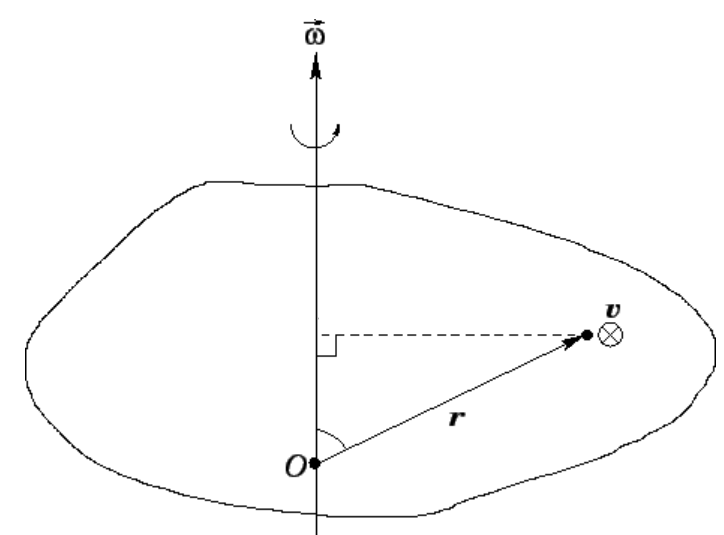
\includegraphics[scale=0.65]{omega.png}
\end{center}
The angular momentum of the rigid body is defined by the following, with $\vec{p}_i$ denoting the linear momentum of the particles constituting the rigid body:
\begin{align*}
\vec{L} = \sum_i \vec{L}_i \coloneqq \sum_i \vec{r}_i \times \vec{p}_i = \sum_i m_i(\vec{r}_i \times \vec{v}_i) = \sum_i m_i \left( \vec{r}_i \times \left(\vec{\omega}\times \vec{r}_i\right)\right) = \sum_i m_i \left( \vec{\omega}r_i^2 - \vec{r}_i \left( \vec{\omega} \cdot \vec{r}_i\right) \right) \tag{AM}
\end{align*}
Note here $\vec{L}$ depends on the choice of the origin, the origin is usually chosen to be a point where the body is fixed when rotating, or the center of mass of the body. \\

By equation (AM), we also observer that $\vec{L}$ is along the direction of $\vec{\omega}$ if and only if $\sum_i m_i\vec{\omega}\cdot \vec{r}_i = 0$, that is, if and only if the mass distribution of the rigid body is symmetric with respect to the rotation axis defined by $\vec{\omega}$. In which case, we can define the scalar valued rotational moment of inertia as the following:
\begin{align*}
I = \sum_i m_i r_i^2 \qquad\text{or} \qquad I = \int_V r^2\, dm
\end{align*}
Here $r$ is the distance from the point mass $dm$, or $m_i$, to the rotation axis defined by the direction of $\vec{\omega}$. The kinetic energy of the rigid body in this situation is given by the following:
$$T_{total} = \frac{1}{2}MV^2_{CM} + \frac{1}{2}I \omega^2$$
where $M$ is the total mass of the system, and $V_{CM}$ is the speed of the center of mass.\\

While in general, the mass distribution of the rigid body does not have to be symmetric with respect to its rotation axis defined by $\vec{\omega}$, in such cases we are not able to define the scalar valued moment of inertia $I$. In fact, the quantity rotational inertial can be defined by using a tensor, denoted as $\mathbf{I}$, such that we have the following being satisfied:
\begin{align*}
\vec{L} = \mathbf{I}\cdot \vec{\omega}
\end{align*}
\newpage

One example of the mass distribution of the rigid body not being symmetric with respect to its rotation axis defined by $\vec{\omega}$ is illustrated in the following figure:
\begin{center}
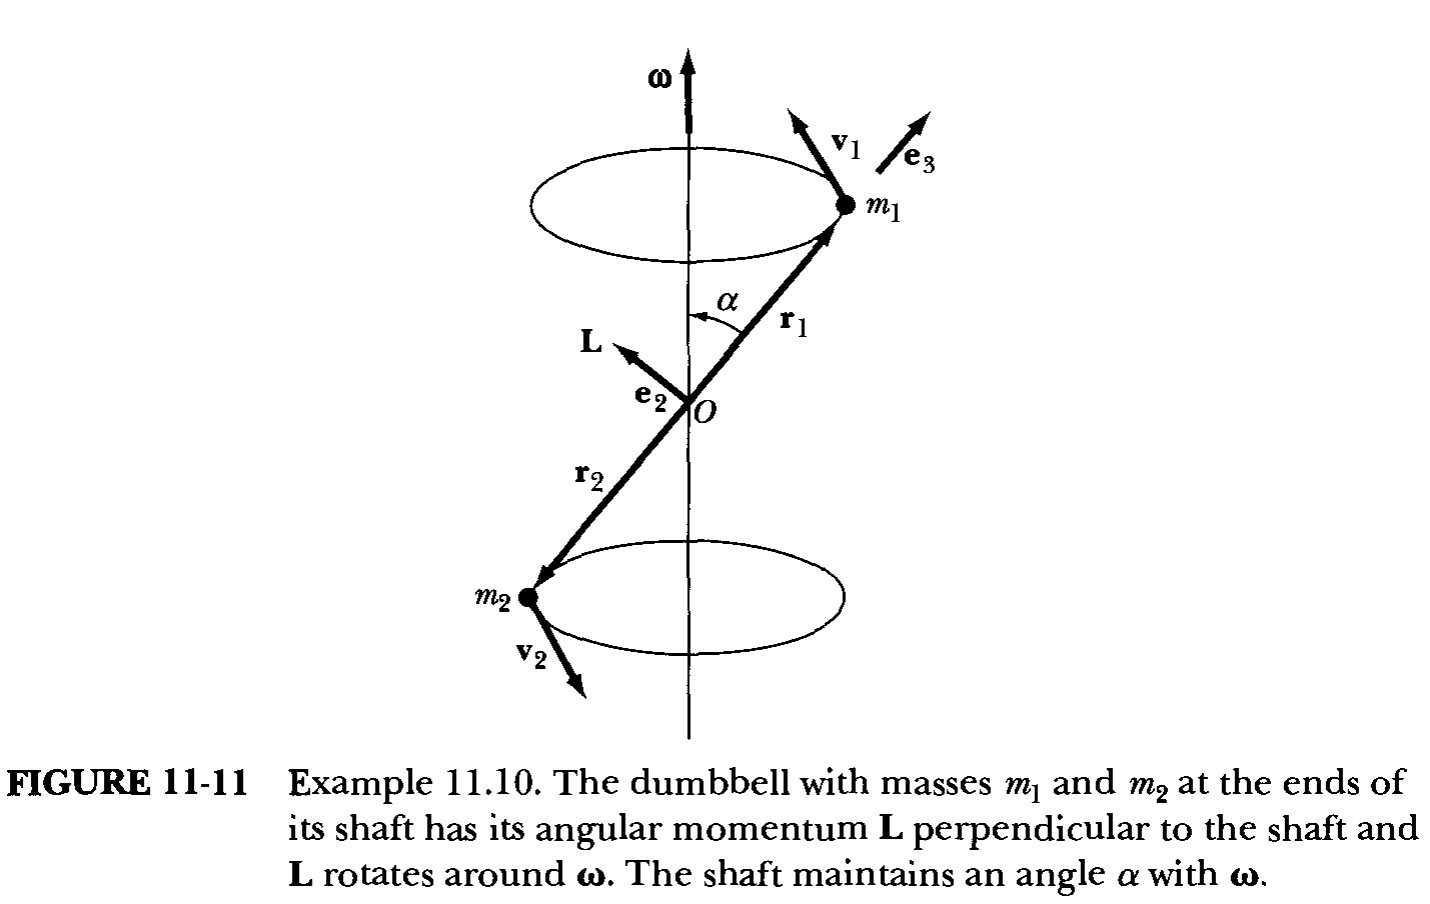
\includegraphics[scale=0.35]{shaft.png}
\end{center}

The real complication is to handle the general rotation of the rigid body when $\vec{\omega}$ is not orthogonal to $\vec{r}_i$, we will develop the equation of motion using a fixed initial coordinate system, and another coordinate system fixed with respect to the rigid body. The coordinate system fixed with respect to the body is rotational as the body itself rotates, hence such coordinate system is a non-inertial reference frame, in particular, a rotational frame, which will be discussed in the next section.\\

Six quantities must be specified to describe the motion of the body. We normally use three coordinates to describe the position of the center of mass of the rigid body, which can often conveniently be made to coincide with the origin of the body coordinate system, and three independent angles that give the orientation of the body coordinate system with respect to the fixed system. The three independent angles are normally taken to be the Eulerian angles.\\


\example
A cylinder with uniform mass distribution, of radius $R$, total mass $M$, height $b$, and mass density $\rho$, rotating around its own axis has rotational inertia given by the following:
\begin{align*}
I_z = \int_0^R \int_0^{2\pi}\int_{-b/2}^{b/2} \rho r^2 \, r\, dr \, d\phi\, dz = \frac{1}{2}MR^2
\end{align*}
note here we have:
\begin{align*}
dm = \rho dV = \frac{M}{\pi R^2 b}\, dr\, d\phi\, dz
\end{align*}
\hfill\break\hfill\break\hfill\break

\subsection*{Non-inertial Reference Frame}
It is always possible to express the equations of motion for a system in an inertial frame, but there are types of problems for which these equations would be extremely complex, and it becomes easier to treat the motion of the system in a non-inertial frame of reference.\\

To describe, for example, the motion of a particle on or near the surface of Earth. It is tempting to do so by choosing a coordinate system fixed with respect to Earth. We know, however, that the Earth undergoes a complicated motion, compounded of many different rotations, hence accelerations, with respect to an inertial reference frame identified with the fixed stars. Earth's coordinate system is therefore a non-inertial frame of reference. Although  the solutions to many problems can be obtained to the desired degree of accuracy by ignoring this distinction, many important effects result from the non-inertial nature of the Earth coordinate system. \\


\section[Rotational Frame]{\color{red} Rotational Frame\color{black}}
Let $S(\hat{e}_x,\hat{e}_y,Z)$ be a fixed inertial frame. Consider a frame $S'(\ihat,\jhat,Z)$, with origin at the position the same as the origin of $S$, and $S'$ rotates about $Z$-axis with angular velocity $\omega$. Denote a point in $S'$ as $\vec{r}(x,y) = x \ihat + y \jhat$. Let $\phi$ be the angle between $\ihat$ and $\vec{e}_x$, then we can write:
\begin{align*}
\ihat  = \cos(\phi) \hat{e}_x + \sin(\phi) \hat{e}_y \qquad\qquad\qquad \jhat = -\sin(\phi)\hat{e}_x + \cos(\phi) \hat{e}_y
\end{align*}
Then we get the following:
\begin{align*}
\frac{d\ihat}{dt} = \dot{\phi} \jhat = \omega \jhat \qquad\qquad\qquad\qquad\qquad \frac{d\jhat}{dt} = -\dot{\phi}\ihat = -\omega \ihat
\end{align*}
For external force $\vec{F}$ acting on a particle with mass $m$ in the fixed frame $S$, the position, velocity, and acceleration of the particle in $S$ are denoted as $\vec{r},$ $\vec{v}$, $\vec{a}$, respectively, and the position, velocity, and acceleration of the particle in $S'$ are denoted as $\vec{r}'$, $\vec{v}'$, and $\vec{a}'$, respectively. Here we can write the following:
\begin{align*}
\vec{v} = \frac{d\vec{r}}{dt} = \dot{x}\ihat + \dot{y}\jhat + x \frac{d\ihat}{dt}+ y \frac{d\jhat}{dt} = \dot{x}\ihat + \dot{y}\jhat + \omega(x\jhat - y\ihat) = \vec{v}' + \vec{\omega}\times \vec{r}
\end{align*}
where we have $\vec{v}' = \dot{x}\ihat + \dot{y}\jhat$, and $(\omega \hat{Z} )\times (x\ihat + y\jhat) = \omega (x\jhat - y\ihat)$. Here we can write the following:
\begin{align*}
\vec{a} = \frac{d\vec{v}}{dt} &= \frac{d\vec{v}'}{dt} + \vec{\omega}\times \vec{v}' + \frac{d\vec{\omega}}{dt} \times \vec{r}+ \vec{\omega }\times \frac{d\vec{r}}{dt}\\
&= \frac{d\vec{v}'}{dt} + \vec{\omega}\times \vec{v}' + \frac{d\vec{\omega}}{dt} \times \vec{r}+ \vec{\omega }\times (\vec{v}' + \vec{\omega}\times \vec{r})\\
&=\vec{a}' + 2\vec{\omega}\times \vec{v}' + \frac{d\vec{\omega}}{dt} \times \vec{r}+ \vec{\omega }\times (\vec{\omega}\times \vec{r})\\
\tag{AF}
\end{align*}
Here we note that, in general, for any $\vec{Q}$ rotates in a fixed system with angular velocity $\vec{\omega}$, we have:
\begin{align*}
\left(\frac{d\vec{Q}}{dt} \right)_{\text{fixed frame}} = \left(\frac{d\vec{Q}}{dt} \right)_{\text{rotational frame}} + \vec{\omega}\times \vec{Q} \tag{RF}
\end{align*}
\begin{align*}
\left(\frac{d\vec{\omega}}{dt} \right)_{\text{fixed frame}} = \left(\frac{d\vec{\omega}}{dt} \right)_{\text{rotational frame}} + \vec{\omega}\times \vec{\omega} = \dot{\omega}
\end{align*}

From equation (AF), we obtain the following:
\begin{align*}
\vec{F} = m\vec{a} = m\vec{a}' + 2m\vec{\omega}\times \vec{v}' + m\frac{d\vec{\omega}}{dt} \times \vec{r}+m\vec{\omega }\times (\vec{\omega}\times \vec{r})
\end{align*}
It follows that, in $S'$, the external force $\vec{F}'$ experienced by the particle is given by the following:
\begin{align*}
\vec{F}' = m\vec{a}' = \vec{F} - m \frac{d\vec{\omega}}{dt}\times \vec{r} - m \vec{\omega} \times (\vec{\omega} \times \vec{r}) - 2m \vec{\omega}\times \vec{v}'
\end{align*}
The term $-2m \vec{\omega}\times \vec{v}'$ is known as the Coriolis force, and the term $-m\vec{\omega}$ is known as the Centrifugal force. In physics, the Coriolis force is an inertial, or fictitious force, that acts on objects that are in motion within a frame of reference that rotates with respect to an inertial frame. The Coriolis force is proportional to the rotation rate and the Centrifugal force is proportional to the square of the rotation rate. In usual case, Centrifugal force points in the direction direct away from the axis of rotation. \\
\newpage

\section[Angular Momentum and Inertia Tensor]{\color{red} Angular Momentum and Inertia Tensor\color{black}}
Consider a multiple particle rigid body $\{\text{partiacle }i \text{ of mass }m_i \text{ at position }\vec{r}_i\}$, rotates around an axis $\vec{\omega}$. Here $\vec{r}_i$ is measured with respect to the origin $O$. Then we can write the following:
\begin{align*}
\vec{L} = \sum_i \vec{L}_i = \sum_i m_i \left( \vec{r}_i \times \left(\vec{\omega}\times \vec{r}_i\right)\right) = \sum_i m_i \left( \vec{\omega}r_i^2 - \vec{r}_i \left( \vec{\omega} \cdot \vec{r}_i\right) \right)
\end{align*}
Denote $\vec{L} = (L_x,L_y,L_z)$, and denote $\vec{r}_i = (x_i, y_i, z_i)$, $\omega = (\omega_x, \omega_y,\omega_z)$, we can write:
\begin{align*}
L_x = \omega_x \sum_i m_i (y_i^2 + z_i^2)  - \omega_y \sum_i m_i x_i y_i - \omega_z \sum_i m_i x_i z_i
\end{align*}
\begin{align*}
L_y = \omega_y \sum_i m_i (z_i^2 + x_i^2)  - \omega_x \sum_i m_i y_i x_i - \omega_z \sum_i m_i y_i z_i
\end{align*}
\begin{align*}
L_z = \omega_z \sum_i m_i (x_i^2 + y_i^2)  - \omega_x \sum_i m_i z_i x_i - \omega_y \sum_i m_i z_i y_i
\end{align*}

Here we define the inertial tenser:
\begin{align*}
\mathbf{I} \coloneqq \begin{bmatrix}
I_{xx} & I_{xy} & I_{xz} \\
I_{yx} & I_{yy} & I_{yz}\\
I_{zx} & I_{zy} & I_{zz}
\end{bmatrix}
\end{align*}
where we have:
\begin{align*}
I_{xx} = \sum_i m_i (y_i^2 + z_i^2) \qquad \qquad I_{yy} = \sum_i m_i(z_i^2 + x_i^2) \qquad\qquad I_{zz} = \sum_i m_i (x_i^2 + y_i^2)
\end{align*}
\begin{align*}
I_{xy} = I_{yx} = -\sum_i m_i x_i y_i \qquad \quad I_{yz} = I_{zy} = -\sum_i m_i y_i z_i \qquad\quad I_{zx} = I_{xz} = -\sum_i m_i z_i x_i
\end{align*}
For continuous mass distribution, $\vec{r} = (r_1, r_2, r_3)$. Let $\{i,j,k\} = \{1,2,3\}$, we write:
\begin{align*}
I_{ii} = \int (r_j^2 + r_k^2) \, dm \qquad \qquad I_{ij} = -\int r_ir_j\, dm
\end{align*}
Combining, one can show that we have:
\begin{align*}
\vec{L} = \mathbf{I}\cdot \vec{\omega} = \begin{bmatrix}
L_x \\ L_y \\ L_z
\end{bmatrix} = 
\begin{bmatrix}
I_{xx} & I_{xy} & I_{xz} \\
I_{yx} & I_{yy} & I_{yz}\\
I_{zx} & I_{zy} & I_{zz}
\end{bmatrix} 
\begin{bmatrix}
\omega_x \\ 
\omega_y \\
\omega_z
\end{bmatrix}
\end{align*}
Here $I_{ii}$ is called the moment of inertia about the axis $i$, and $I_{ij}$ is called the products of inertia.\\

For a rigid body defined by \text{particle }$i$ \text{ of mass }$m_i$ \text{ at position }$\vec{r}_i$ with origin $O$ rotates around the point $O$ with an angular velocity  $\vec{\omega}$, the total kinetic rotational energy is given by:
\begin{align*}
T_{rot}
&= \frac{1}{2}\sum_i m_i \vec{v}_i^2 \\
&= \frac{1}{2}\sum_i m_i \vec{v}_1 \cdot (\vec{\omega}\times \vec{r}_i) \\
&= \frac{1}{2}\vec{\omega} \cdot \left(\sum_i \vec{r}_i \times (m_i \vec{v}_i)\right)\\ 
&= \frac{1}{2}\vec{\omega}\cdot \vec{L} \\
&= \frac{1}{2}\vec{\omega} \cdot \left(\mathbf{I}\cdot \vec{\omega}\right) \\
\end{align*}
Expanding in components of $\vec{\omega}$ and $\vec{L}$:
\begin{align*}
T_{\text{rot}} =  \frac{1}{2}\vec{\omega} \cdot \left(\mathbf{I}\cdot \vec{\omega}\right) &= \frac{1}{2}(\omega_x L_x + \omega_y L_y + \omega_z L_z) 
\end{align*}
Moreover, if $\vec{L}$ is along the the direction of $\vec{\omega}$, then there exists scalar-valued $I$ such that we can write the following:
\begin{align*}
T_{\text{rot}} = \frac{1}{2}\,\vec{\omega}\cdot (\mathbf{ I} \cdot \vec{\omega}) = \frac{1}{2}\,I \omega^2
\end{align*}
\newpage
\section[Principal Axes of Inertia]{\color{red} Principal Axes of Inertia\color{black}}
If an inertial tensor $\mathbf{I}$ satisfies the condition that $I_{ij}$ vanishes when $i \neq j$, then $\mathbf{I}$ is said to be diagonal. In which case we can write the following:
\begin{align*}
\bmat{L_x \\ L_y \\L_z} = \bmat{I_{xx} & 0 & 0 \\
0 & I_{yy} & 0 \\
0 & 0 & I_{zz}} \bmat{\omega_x \\ \omega_y \\ \omega_z} = \bmat{I_{xx}\omega_x \\ I_{yy}\omega_y \\ I_{zz}\omega_z} \tag{PL}
\end{align*}
\begin{align*}
T_{\text{rot}} = \frac{1}{2}\sum_{i} I_{ii}\omega_i^2
\end{align*}
Here we see that the condition where $\mathbf{I}$ has only diagonal elements provides quite simple expressions for the angular momentum and hence for the rotational kinetic energy, we now want to determine the conditions when $\mathbf{I}$ is diagonal. This involves finding a coordinate system for which the products of inertia, which are the off-diagonal elements of $\mathbf{I}$, vanish. We call the axes of such coordinate system the principal axes of inertial of the rigid body.\\

\note The coordinate system constructed by the principle axes of the rigid body will rotate as the rigid body rotates. That is, the frame constructed by the principle axes of the rigid body is a rotational frame, and it rotates with the body itself. \\


If a body rotates around a principal axis, both the angular velocity and the angular momentum are directed along such axis because we have $L_i = I_{ii}\omega_i$ by equation (PL). Hence the process of finding the principle of axes corresponds to finding the eigenvalues of the matrix $\mathbf{I}$ and their corresponding eigenvectors. For eigenvalue $I$ of $\mathbf{I}$, we requires the following holds:
\begin{align*}
\vec{L} = \mathbf{I}\cdot \vec{\omega} = I \vec{\omega} \qquad \Rightarrow \qquad (\mathbf{I} - I \cdot \mathbf{Id}) = 0
\end{align*}
where $\mathbf{Id}$ is the $3\times 3$ identity matrix, and this requires the following holds:
\begin{align*}
\det\left(\begin{bmatrix}
I_{xx}-I & I_{xy} & I_{xz} \\
I_{yx} & I_{yy}-I & I_{yz}\\
I_{zx} & I_{zy} & I_{zz}-I
\end{bmatrix}  \right) = 0
\end{align*}
Since $\mathbf{I}$ is symmetric, it is always diagonalizable, hence one can always find eigenvalues for $\mathbf{I}$ and their corresponding eigenvectors.\\

Any set of unit linearly independent eigenvectors of $\mathbf{I}$ can be used to construct the principle of axes of the object. That is, if $\vec{\omega}_1$ is an eigenvector corresponding to the  eigenvalue $I_i$ of $\mathbf{I}$, then the direction of $\vec{\omega}$ with respect to the object coordinate system is then the same as the direction of the principal axis corresponding to $I_1$. Therefore, we can determine the direction of principal axes by examining the eigenspaces of the eigenvalues of $\mathbf{I}$. For eigenspace of dimension greater than $1$, one can use Gram-Schmidt Orthonormalization Process to obtain a set of orthonormal eigenvectors corresponding to such eigenvalue. Here by standard Linear Algebra results, the principal axes determined in this manner are indeed real and orthogonal as the eigenvectors are orthonormal.\\

Since $\mathbf{I}$ is diagonalizable, we can denote the three eigenvalues of $\mathbf{I}$ as $I_1$, $I_2$, and $I_3$. If we have $I_1 = I_2 = I_3$, the rigid body is termed as a spherical top. If $I_1 = I_2 \neq I_3$, the rigid body is termed as a symmetric top. If the principal moments of inertia, $I_1$, $I_2$, $I_3$, are all distinct, then the rigid body is termed as an asymmetric top. If we have $I_1 = 0$, and $I_2 = I_3$, then the body is called a rotor. 

\newpage
\section[Equations of Motions for a Rigid Body]{\color{red}Equations of Motions for a Rigid Body\color{black}}

By equation (RF), for angular momentum $\vec{L}$, we can write the following:
\begin{align*}
\left(\frac{d\vec{L}}{dt}\right)_{\text{fixed frame}}  = \left(\frac{d\vec{L}}{dt}\right)_{\text{rotational frame}}+ \vec{\omega}\times \vec{L} \tag{RFL}
\end{align*}
where $\vec{\omega}$ is the angular velocity of the rotating rigid body.\\

Let $(\ihat, \jhat, \hat{\text{k}})$ be the set of the orthonormal vectors corresponding to the principal axes of a rotational rigid body. The coordinate system constructed by $(\ihat, \jhat, \hat{\text{k}})$ is called the rotational frame, or the body coordinate system in this section. The rigid body equations of motion are most convenient expressed in the body coordinate system. Let $I_1$, $I_2$, and $I_3$ denote the eigenvalues of the inertial tensor $\mathbf{I}$ of the rigid body, corresponding to eigenvectors $\ihat,$ $\jhat$, and $\khat$, respectively. \\

Let $\vec{L} = (L_1,L_2,L_3)$ denote the angular momentum of the rigid body in rotational frame, and let $\vec{\omega}= (\omega_1, \omega_2, \omega_3)$ denote the angular velocity of the rigid body in the rotational frame. Here the angular momentum of the object can be written as the following:
\begin{align*}
\vec{L} = L_1 \ihat + L_2 \jhat + L_3 \khat = I_1 \omega_1 \ihat + I_2 \omega_2 \jhat + I_3 \omega_3 \khat
\end{align*}
Applying equation (RFL), we can write the following:
\begin{align*}
\vec{N} = \left(\frac{d\vec{L}}{dt}\right)_{\text{fixed frame}} = \left(\frac{d\vec{L}}{dt}\right)_{\text{rotational frame}} + \vec{\omega}\times \vec{L} = \dot{L}_1 \ihat + \dot{L}_2\jhat + \dot{L}_3 \khat + \vec{\omega}\times \vec{L}
\end{align*}
Let $\vec{N} = (N_1, N_2, N_3)$ denote the torque on the rigid body in the rotational frame, we can write:
\begin{align*}
\begin{cases}
N_1 = I_1 \dot{\omega}_1 - (I_2-I_3)\omega_2 \omega_3 \\
N_2 = I_2 \dot{\omega}_2 - (I_3 - I_1) \omega_3 \omega_1 \\
N_3 = I_3 \dot{\omega}_3 - (I_1 - I_2) \omega_1 \omega_2
\end{cases} \tag{EMR}
\end{align*}
Here equation (EMR) gives the equation of motion in the body coordinate system, equation (EMR) is also called the Euler's Equations of motion for the rigid body. The issue remaining here is that $\vec{\omega}$ is difficult to be determined in the rotational frame, we need to represent $\omega_1,\, \omega_2,\, \omega_3$ with quantities that can be measured in the fixed frame.\\

\subsection*{Eulerian Angles}
First we want to find a way to transform the coordinates in the fixed frame to coordinates in the rotational frame. Let $\vec{x}'$ be a coordinate in the fixed frame, let $(x_1', x_2', x_3')$ be the family of axes of the fixed frame, let $\vec{x}$ denote a coordinate in the rotational frame, and let $(x_1, x_2, x_3)$ the family of axes of the rotational frame. The coordinate system constructed by the family of axes $(x_1', x_2', x_3')$ is called the $x_i'$ system, and similarly the coordinate system constructed by the family of axes $(x_1, x_2, x_3)$ is called the $x_i$ system. The transformation from one coordinate system to another can be represented by a matrix equation of the form: \footnote{TO BE CONSISTENT with the textbook \textit{Classical Dynamics of Particles and Systems} by Stephen T. Thornton and Jerry B. Marion, here we use $x_i$ and $x_i'$ to denote the axes, they are neither components of the vectors $\vec{x}$ and $\vec{x}$', nor orthonormal vectors defining the axes, that is, $\vec{x} \neq (x_1,x_2,x_3)$, and $\vec{x}' \neq (x_1', x_2', x_3')$. That is, $x_i$ and $x_i'$ are simply notation for the axes of the systems. This notation is confusing, but just to be consistent with the textbook.}
\begin{align*}
\vec{x} = \lambda \vec{x}'
\end{align*}
where $\lambda$ is a $3\times 3$ matrix.\\


To find matrix $\lambda$, we find it convenient to use the Eulerian angles $\phi$, $\theta$, and $\psi$, which are generated in the following series of rotations, which takes the $\vec{x}'$ coordinate system  to $\vec{x}$ coordinate system:
\begin{enumerate}
\item The first rotation is counter clockwise through an angle $\phi$ about the $x_3'$-axis to transform the $x_i'$ system to the $x_i''$ system.\footnote{Again, $(x_1'', x_2'', x_3'')$ and $(x_1', x_2', x_3')$ are families of axes, they are not vectors, nor components of vectors. We use this notation just to be consistent with the textbook. Here $x_i$ system refers to the coordinate system constructed by the family of axes $(x_1, x_2, x_3)$, and $x_i'$ system refers to the coordinate system constructed by the family of axes $(x_1', x_2', x_3')$.} Here we get the transformation matrix $\lambda_{\phi}$ given by the following:
\begin{align*}
\lambda_{\phi} = \bmat{\cos(\phi) & \sin(\phi) & 0 \\ -\sin(\phi) & \cos(\phi) & 0 \\ 0 & 0 &1} 
\end{align*}
for coordinate $\vec{x}'$ in the $x_i'$ system and $\vec{x}''$ in the $x_i''$ system, we can write:
\begin{align*}
\vec{x}'' = \lambda_{\phi} \vec{x}'
\end{align*}
\item The second rotation is counterclockwise through an angle $\theta$ about the $x''_1$-axis to transform the $x_i''$ system to the $x_i'''$ system. Here we get the transformation matrix $\lambda_{\theta}$ given by the following:
\begin{align*}
\lambda_{\theta} = \bmat{1 & 0 & 0 \\ 0 &\cos(\theta) & \sin(\theta) \\ 0 & -\sin(\theta) & \cos(\theta)} 
\end{align*}
for coordinate $\vec{x}''$ in the $x_i''$ system and $\vec{x}'''$ in the $x_i'''$ system, we can write:
\begin{align*}
\vec{x}''' = \lambda_{\theta} \vec{x}''
\end{align*}
\item The third rotation is counterclockwise through an angle $\psi$ about the $x_3'''$-axis to transform the $x_i'''$ system to the $x_i$ system. Here we get the transformation matrix $\lambda_{\psi}$ given by the following: 
\begin{align*}
\lambda_{\psi} = \bmat{\cos(\psi) & \sin(\psi) & 0 \\ -\sin(\psi) & \cos(\psi) & 0 \\ 0 & 0 &1}
\end{align*}
for coordinate $\vec{x}$ in the $x_i$ system and $\vec{x}'''$ in the $x_i'''$ system, we can write: \footnote{TO BE CLEAR one more time, here $(x_1,x_2,x_3)$, $(x_1''',x_2''',x_3''')$, $(x_1'',x_2'', x_3'')$, and $(x_1',x_2',x_3')$ are four families of axes. They are not families of vectors, nor vectors, nor families of components of vectors. That is, $x_1$, $x_2'$, $x_3''$ are axes, and $\vec{x} \neq (x_1,x_2,x_3)$. Here $x_i$ system refers to the coordinate system constructed by the family of axes $(x_1,x_2,x_3)$, and $x_i'''$ system refers to the the coordinate system constructed by the family of axes $(x_1''',x_2''',x_3''')$.}
\begin{align*}
\vec{x} = \lambda_{\psi} \vec{x}'''
\end{align*}
\end{enumerate}
Here the three rotations are illustrated in the following figure:
\begin{center}
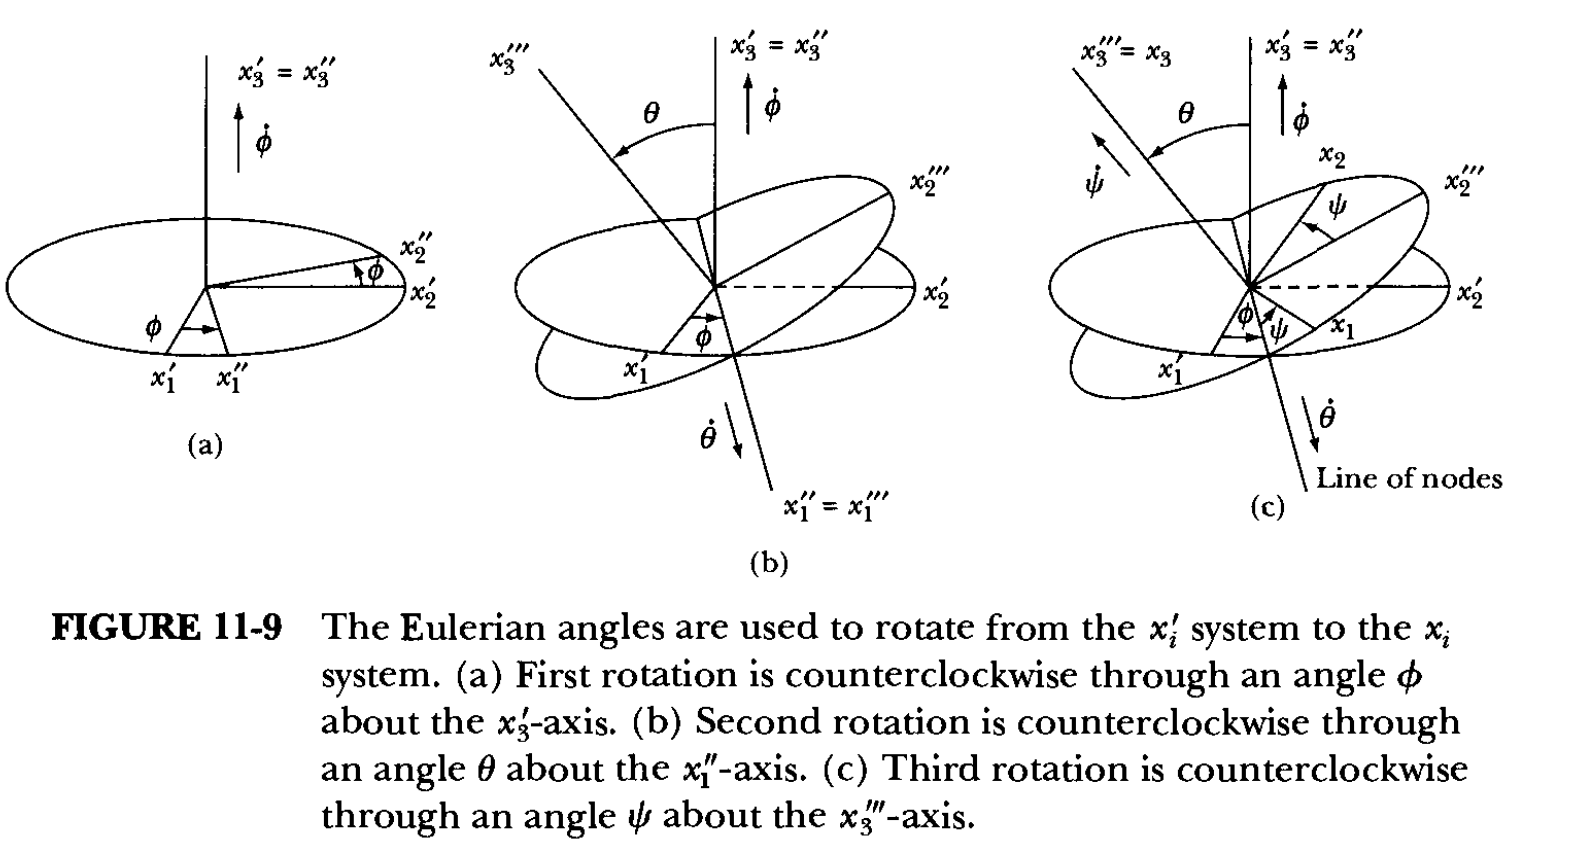
\includegraphics[scale=0.35]{eulerian.png}
\end{center}
The line common to the planes containing the $x_1$- and $x_2$-axes and the $x'_1$- and $x_2'$-axes is called the line of nodes. The complete transformation matrix from the $(x_1',x_2',x_3')$-frame to the $(x_1,x_2,x_3)$-frame is given by the following:
\begin{align*}
\lambda = \lambda_{\psi} \lambda_{\theta}\lambda_{\phi}
\end{align*}
For coordiante $\vec{x}$ in the $(x_1,x_2,x_3)$-frame, and coordinate $\vec{x}'$ in the $(x_1',x_2',x_3')$-frame, we can write:
\begin{align*}
\vec{x} = \lambda_{\psi}\lambda_{\theta}\lambda_{\phi} \vec{x}' 
\end{align*}


Let $\lambda_{ij}$ denote the $ij$-entry in the matrix $\lambda$, we can write:
\begin{align*}
\lambda_{11} &= \cos(\psi) \cos(\phi) - \cos(\theta) \sin(\phi) \sin(\psi)  \\
\lambda_{21} &= -\sin(\psi) \cos(\phi) - \cos(\theta) \sin(\phi) \cos(\psi) \\
\lambda_{31} &= \sin(\theta) \sin(\phi)\\
\lambda_{12} &= \cos(\psi)\sin(\phi) + \cos(\theta) \cos(\phi) \sin(\psi)\\
\lambda_{22} &= -\sin(\psi) \sin(\phi) +\cos(\theta) \cos(\phi) \cos(\psi)\\
\lambda_{32} &= -\sin(\theta) \cos(\phi)\\
\lambda_{13} &= \sin(\psi) \sin(\theta)\\
\lambda_{23} &= \cos(\psi) \sin(\theta) \\
\lambda_{33} &= \cos(\theta)
\end{align*}

Here we note that the body coordinate system is a rotational frame, hence $\theta, \phi, \psi$ are functions of time, and the angular velocity of the rigid body in the body coordinate system, denoted as $\vec{\omega} = (\omega_1,\omega_2,\omega_3)$, can be expressed as the following:
\begin{align*}
\vec{\omega} = (\dot{\phi}_1+ \dot{\theta}_1 + \dot{\psi}_1,\  \dot{\phi}_2+ \dot{\theta}_2 + \dot{\psi}_2, \ \dot{\phi}_3+ \dot{\theta}_3 + \dot{\psi}_3)
\end{align*}
where, in the rotational $(x_1,x_2,x_3)$-frame, we denote denote $\dot{\phi} = (\dot{\phi}_1, \dot{\phi}_2,\dot{\phi}_3)$, $\dot{\theta} = (\dot{\theta}_1, \dot{\theta}_2,\dot{\theta}_3)$, $\dot{\psi} = (\dot{\psi}_1, \dot{\psi}_2,\dot{\psi}_3)$. By geometry of indicated in Figure 11-9, we can write the following:
\begin{align*}
\begin{cases}
\dot{\phi}_1 = \dot{\phi} \sin(\theta) \sin(\psi)\\ \dot{\phi}_2 = \dot{\phi} \sin(\theta) \cos(\psi)\\
\dot{\phi}_3 = \dot{\phi}\cos(\theta)
\end{cases}
\qquad\qquad
\begin{cases}\dot{\theta}_1 = \dot{\theta} \cos(\psi) \\
\dot{\theta}_2 = -\dot{\theta}\sin(\psi) \\
\dot{\theta}_3 = 0\\
\end{cases}
\qquad\qquad
\begin{cases}
\dot{\psi}_1 = 0\\
\dot{\psi}_2 = 0\\
\dot{\psi}_3 = \dot{\psi}
\end{cases}
\end{align*}
Combining, and denote $\vec{\omega} = (\omega_1, \omega_2,\omega_3)$ in the body coordinate system, we get the following:
\begin{align*}
\omega_1 &= \dot{\phi}\sin(\theta)\sin(\psi) + \dot{\theta}\cos(\psi)\\
\omega_2 &= \dot{\phi}\sin(\theta) \cos(\psi) - \dot{\theta}\sin(\psi) \\
\omega_3 &= \dot{\phi}\cos(\theta) + \dot{\psi}
\end{align*}
First we observe that, the quantity $\vec{\omega}$ in the body coordinate system is not necessarily fixed when the rigid body is rotating. One can similarly show that $\vec{\omega}$ is not necessarily fixed in the fixed coordinate system. \\

Now we can choose the Eulerian angle $\phi$, $\theta$, and $\psi$  such that the body frame constructed by the Eulerian angles coincide with the body frame constructed by the principal axes of the rigid body,  in which case equation (EMR) can now be evaluated using quantities $\psi$, $\theta$, and $\psi$ measured in the fixed frame. Moreover, we also obtain the rotational kinetic energy of the rigid body in the rotational frame is given by the following:
\begin{align*}
T_{rot}= \frac{1}{2}\sum_i I_i \omega_i^2
\end{align*}

\subsection*{Force-free Motion of a Symmetric Spinning Top}
Consider a symmetric top, which is a rigid body with $I_1 = I_2 \neq I_3$. Here $\vec{\omega} = (\omega_1,\omega_2,\omega_3)$ denote the angular velocity of the rigid body in the body coordinate system constructed by the principal axes of the rigid body. Here we denote the three axes of the body coordinate system as $x_1$, $x_2$, and $x_3$, which are the principal axes corresponding to $I_1$, $I_2$, $I_3$, respectively, and $I_1$, $I_2$, $I_3$ are the eigenvalues of the inertial tenser $\mathbf{I}$ of the rigid body. Since we are assuming force free motion, the rigid body experience no force, and hence no torque. In the body coordinate system, torque on the body is zero, so $\vec{N} = (N_1,N_2,N_3) = (0,0,0)$ gives the torque on the rigid body in the body coordinate system. Then the force-free Euler Equations is given by the following:
\begin{align*}
\begin{cases}
(I_1 - I_3) \omega_2 \omega_3 - I_1 \dot{\omega}_1 = 0 \\
(I_3 - I_1) \omega_3 \omega_1 - I_1\dot{\omega}_2 = 0 \\ 
I_3 \dot{\omega}_3 = 0
\end{cases} \tag{FFM}
\end{align*}
Since for force-free motion the center of mass of the body is either at rest or in uniform motion with respect to the fixed frame, we can, without loss of generality, specify that the body's center of mass is at rest and located at the origin of the fixed coordinate system. We consider the case in which the angular velocity $\vec{\omega}$ does not lie along a principal axis of the body, otherwise the motion is trivial.\\

From equation (FFM), we immediately get that $\omega_3$ is constant. Now rearranging equation (FFM) we get:
\begin{align*}
\begin{cases}
0 = \dot{\omega}_1 +\Omega \omega_2 \\
0=\dot{\omega}_2 - \Omega \omega_1 
\end{cases}\qquad\qquad\text{where }\ \ \Omega =\frac{I_3 - I_1}{I_1}\,\omega_3 
\end{align*}
hence we can write:
\begin{align*}
(\dot{\omega}_1 + i \dot{\omega}_2 ) - i \Omega (\omega_1 + i \omega_2) = 0
\end{align*}
Define $\eta \coloneqq \omega_1 + i\omega_2$, we get the following:
\begin{align*}
\dot{\eta} - i \Omega \eta = 0 \qquad \Rightarrow \qquad \eta(t) = Ae^{i\Omega t}
\end{align*}
hence we obtain $\omega_1$ and $\omega_2$ as functions of time by examining $\eta$:
\begin{align*}
\omega_1 + i \omega_2 = A\cos(\Omega t) + iA \sin(\Omega t) \qquad \Rightarrow \qquad \begin{cases}
\omega_1 (t) = A\cos(\Omega t) \\
\omega_2(t) = A\sin(\Omega t)
\end{cases} \tag{FFP}
\end{align*}
Note that $\omega_3$ is a constant, we obtain the following:
\begin{align*}
|| \vec{\omega} || = \sqrt{ \omega_1^2 + \omega_2^2 + \omega_3^3} = \sqrt{A^2 + \omega_3^2} = \text{constant}
\end{align*}
From equation (FFP), in the body coordinate system, we observe that the projection of $\vec{\omega}$ onto the $x_1x_2$-plane describes a circle, parametrized by equation (FFP) with an angular frequency $\Omega$. Here we found that the angular velocity vector $\vec{\omega}$ revolves, or precesses, about the body $x_3$-axis with a constant angular frequency $\Omega$, hence $\Omega$ is called the precession angular frequency of the angular velocity $\vec{\omega}$ around the body symmetric axis $x_3$. \\
\begin{center}
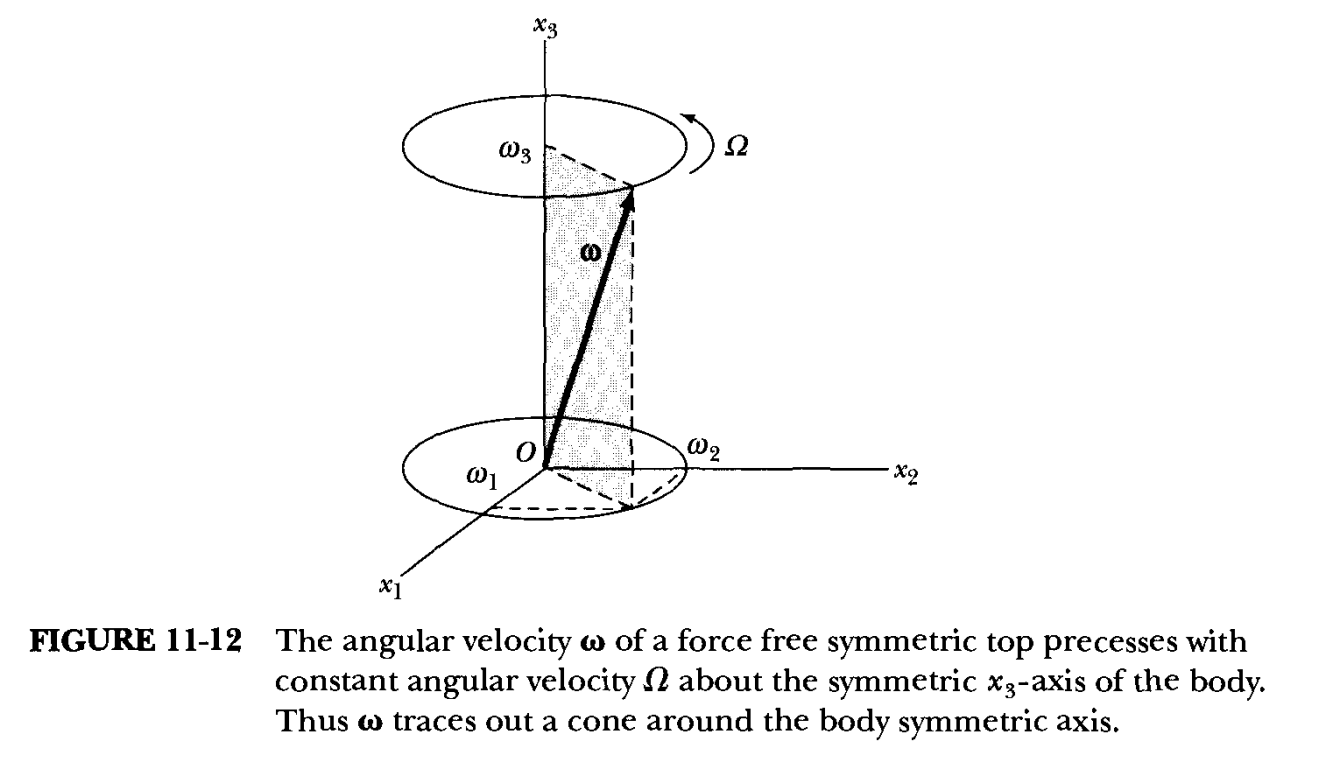
\includegraphics[scale=0.39]{FFsymmetricTop.png}
\end{center}

To an observer in the body coordinate system, $\vec{\omega}$ traces out a cone around the body symmetry axis, called the body cone. \\

Since we are considering force-free motion, the angular momentum vector $\vec{L}$ is stationary in the fixed coordinate system and is constant in time. Note that the kinetic energy is also a constant. In particular, the rotational kinetic energy is constant because the we assumed that the center of mass of the rigid body is at rest in the fixed frame, hence we have:
\begin{align*}
T_{\text{rot}} = \frac{1}{2}\vec{\omega}\cdot \vec{L} = \text{constant}
\end{align*}
Hence in the fixed frame, $\vec{\omega}$ must move such that its projection on the stationary angular momentum vector $\vec{L}$ is constant, that is, $\vec{\omega}$ precesses around and makes a constant angle with $\vec{L}$ in the fixed frame. \\


Let $\vec{e}_1,\vec{e}_2,\vec{e}_3$ denote the orthonromal vectors corresponding to the three axes $x_1, x_2, x_3$. Note further that $\vec{L}$, $\vec{\omega}$, and $x_3$-axis all lie in the same plane, this can be shown by the following by noting that $I_1 = I_2$ for symmetric top:
\begin{align*}
\vec{L}\cdot (\vec{\omega} \times \vec{e}_3 ) = \vec{L}\cdot (\omega_2 \vec{e}_1 - \omega_1 \vec{e}_2) = I_1 \omega_1 \omega_2 - I_2 \omega_1 \omega_2 = 0
\end{align*}
Therefore, if we designate the $x_3'$-axis in the fixed frame to coincide with the direction of $\vec{L}$, then to an observer in the fixed frame, $\vec{\omega}$ trances out a cone around the fixed $x_3'$-axis, called the space cone. Now the situation is described by one cone, the body cone, rolling on another, the space cone. $\vec{\omega}$ precesses around the $x_3$-axis in the body coordinate system and around the $x_3'$-axis in the fixed frame. Note that the rate at which $\vec{\omega}$ precesses around the body symmetry axis is given by:
\begin{align*}
\Omega = \frac{I_3 - I_1}{I_1}\, \omega_3
\end{align*}
\begin{center}
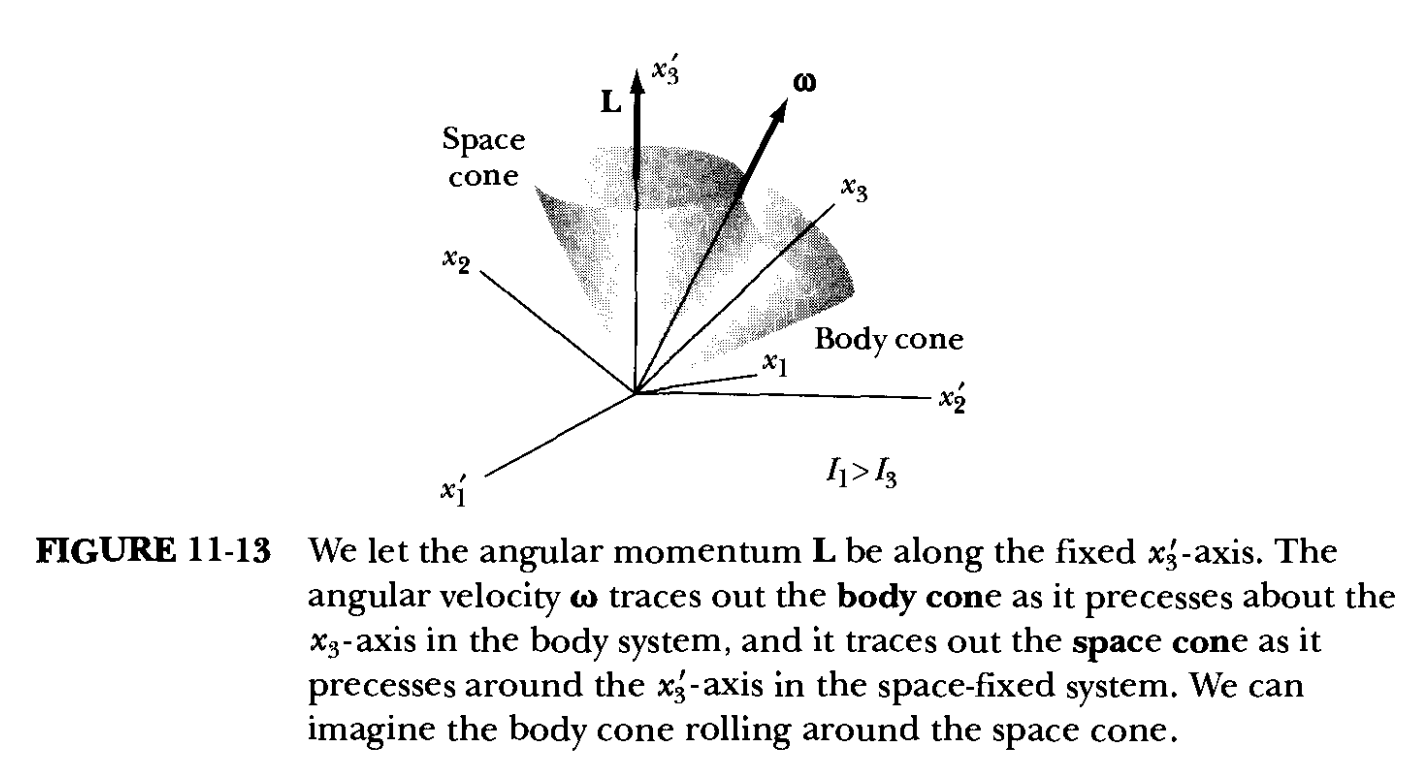
\includegraphics[scale=0.39]{cones.png}
\end{center}

\newpage
\chapter{Coupled Oscillations}
Here we consider a conservative system described in terms of a set of generalized coordinates $\{q_k\mid 1 \leq k \leq n\}$ and with time variable $t$. Such system has $n$ degrees of freedom. We specify that a configuration of stable equilibrium exists for the system and that at equilibrium the, the generalized coordinates have values $q_{k0}$. In such a configuration, the kinetic energy of the system in terms of generalized coordinates can be shown to satisfy the following:
\begin{align*}
T = \frac{1}{2} \sum_{j,k}m_{jk}\dot{q}_j \dot{q}_k
\end{align*}
where $m_{jk}$ are some constant coefficients. Note here, at equilibrium, we have $\dot{q}_k = 0$, hence at equilibrium we would have the following holds:
\begin{align*}
\left.\frac{\partial T}{\partial q_k}\right|_{eq.} = 0 \qquad \forall \, 1\leq k \leq n
\end{align*}
We may further specify that the generalized coordinates $\{q_k\}$ are measured from the equilibrium positions, that is, setting $q_{k0 } = 0$. In such case, the expansion of the potential energy in a Taylor series about the equilibrium configuration yields the following:
\begin{align*}
U = U_0 + \sum_k \left. \frac{\partial U}{\partial q_k}\right|_{eq.} q_k + \frac{1}{2}\sum_{j,k}\left. \frac{\partial^2 U}{\partial q_j \partial q_k}\right|_{eq.} q_j q_k
\end{align*}
Here without loss of generality, one can choose $U_0 = 0$, and since we are at equilibrium, we have:
\begin{align*}
\left. \frac{\partial U}{\partial q_k}\right|_{eq.} \qquad \forall \, 1\leq k \leq n
\end{align*}
Hence we have left with:
\begin{align*}
U = \frac{1}{2}\sum_{j,k}\left. \frac{\partial^2 U}{\partial q_j \partial q_k}\right|_{eq.} q_j q_k
\end{align*}
Now we define:
\begin{align*}
A_{jk} \coloneqq \left.\frac{\partial^2 U}{\partial q_j \partial q_k}\right|_{eq.}
\end{align*}
Combining, we get the following:
\begin{align*}
T = \frac{1}{2}\sum_{j,k}m_{jk}\dot{q}_{j}\dot{q}_k \qquad\qquad\qquad U=\frac{1}{2}\sum_{j,k}A_{jk}q_jq_k
\end{align*}
Hence the Lagrangian of the system reads the following:
\begin{align*}
\mathcal{L} = T - U = \left( \frac{1}{2}\sum_{j,k}m_{jk}\dot{q}_{j}\dot{q}_k\right) - \left( \frac{1}{2}\sum_{j,k}A_{jk}q_jq_k\right)
\end{align*}
which gives the equation of motions:
\begin{align*}
\frac{\partial \mathcal{L}}{\partial q_j} - \frac{d}{dt}\frac{\partial \mathcal{L}}{\partial \dot{q}_j} = 0 \qquad \Rightarrow \qquad \frac{\partial U}{\partial q_j} + \frac{d}{dt}\frac{\partial T}{\partial \dot{q}_j} = 0
\end{align*}
where we have:
\begin{align*}
\frac{1}{2}\sum_k A_{jk}q_k= \frac{\partial U}{\partial q_j} \qquad\qquad\qquad  \frac{1}{2}\sum_k m_{jk}\dot{q}_k=\frac{\partial T}{\partial \dot{q}_j}
\end{align*}
hence combining we get the following:
\begin{align*}
\sum_k \left(A_{jk}q_k + m_{jk}\ddot{q}_k\right) = 0 \qquad \forall\, 1\leq j \leq n \tag{KEQ}
\end{align*}

We expect the solution to (KEQ) of the form given by the following:
\begin{align*}
q_k (t) = a_k e^{i(\omega t -\delta)} \tag{STK}
\end{align*}
where $a_k$ are real amplitudes and $\delta$ can be determined by the initial conditions, without loss of generality, one can choose proper initial conditions such that $\delta = 0$. Note that only the real part of equation (STK) is of our interest. If the frequency $\omega$ is a real quantity, representing the oscillatory motion of the system.  Indeed, $\omega$ is a real quantity, if not, then $T+U$ contains factors that would increase or decrease monotonically with time, but that violates the assumption that we are dealing with a conservative system.\\

With the assumed solution (STK) to the ODE (KEQ), we get the following:
\begin{align*}
\sum_k (A_{jk} - \omega^2 m_{jk}) a_k = 0\qquad \forall\, 1\leq j \leq n \tag{KWS}
\end{align*}
where the common factor $e^{i(\omega t- \delta)}$ has been canceled. This gives us a set of $n$ linear homogeneous equations that the coefficients $a_k$ must satisfy. Now we can define:
\begin{align*}
\mathbf{A} = 
\bmat{
A_{11} & A_{12} & \cdots & A_{1n} \\
A_{21} & A_{22} & \cdots & A_{2n} \\
\vdots & \vdots & & \vdots\\
A_{n1} & A_{n2} & \cdots & A_{nn} \\
} \qquad\qquad\qquad 
\mathbf{M} = 
\bmat{
m_{11} & m_{12} & \cdots & m_{1n} \\
m_{21} & m_{22} & \cdots & m_{2n} \\
\vdots & \vdots & & \vdots\\
m_{n1} & m_{n2} & \cdots & m_{nn} \\
}
\end{align*}
Then equation (KWS) reads the following:
\begin{align*}
\left(\mathbf{A} - \omega^2 \mathbf{M}\right) \bmat{a_1 \\ a_2 \\ \vdots \\a_n} = 0 \tag{LSK}
\end{align*}
For nontrivial solution to the system given by (LSK), we require the following holds:
\begin{align*}
\det\left(\mathbf{A} - \omega^2 \mathbf{M}\right) = 0 \tag{SEC}
\end{align*} 
Equation (SEC) is called the secular equation of the system, or the characteristic equation of the system. There are in general $n$ roots to equation (SEC), that is, we can label $\omega^2 = \omega_r^2$ with $1\leq r \leq n$ such that each $\omega_r^2$ satisfies equation (SEC). The corresponding $\omega_r$ are called the characteristic frequencies, or eigenfrequencies of the system. In some situations, two or more of the $\omega_r$ can be equal, this is the phenomenon of degeneracy. With each $\omega_r$, one can make use of the system (LSK) to find the corresponding linear space for $\vec{a}_{r} \coloneqq (a_{1r},a_{2r},\cdots, a_{nr})$.  Here we note that the sign of each $\omega_r$ does not affect the determination of the corresponding linear space for $\vec{a}_{r}$. Now we obtain the general solution of $q_k(t)$ as the following:
\begin{align*}
q_k(t) = \sum_{r} c_{r}^+ a_{kr} e^{i \omega_r t} + c_\alpha^- a_{kr}e^{-i\omega_r t}
\end{align*}
where $c_r^+$ and $c_r^-$ are constants determined by the initial conditions. Here we can also define:
\begin{align*}
\eta_r (t) = c_r^+ e^{i \omega_r t} + c_r^- e^{-i \omega_r t}
\end{align*}
In which case we can write:
\begin{align*}
q_k(t) = \sum_r a_{kr}\eta_r(t)
\end{align*}
Note here $\eta_r$ is in fact the solution of the equation:
\begin{align*}
\ddot{\eta}_r + \omega_r^2 \eta_r = 0
\end{align*}
The following system is also satisfied:
\begin{align*}
\bmat{q_1 \\ q_2 \\ \vdots \\ q_n} = \bmat{a_{11} & a_{12} & \cdots & a_{1n}\\
a_{21} & a_{22} & \cdots & a_{2n}\\
\vdots & \vdots & & \vdots\\
a_{n1} & a_{n2} & \cdots & a_{nn}}\bmat{\eta_1 \\\eta_2 \\ \vdots \\ \eta_n} \tag{NMS}
\end{align*}
Here $\{\eta_r\}$ is called the set of normal coordinates for the system. The description of the motion for each normal coordinate $\eta_r$ is called a normal mode. The general motion of the system is a complicated superposition of the normal modes.\\

It is easy to show that we have the following holds:
\begin{align*}
T = \frac{1}{2}\sum_r \dot{\eta}_r \qquad \qquad \qquad U = \frac{1}{2} \sum_r \omega_r^2 \eta_r^2
\end{align*}
hence we have:
\begin{align*}
\mathcal{L} = T-U = \frac{1}{2} \sum_r (\dot{\eta}_r^2 - \omega_r^2 \eta_r^2)
\end{align*}
Note here by examining the expression for $\eta_r$, one can find the relationships of the amplitude and phase between $q_i$. If the system has only two masses, and they oscillate in phase as indicated by the normal mode $\eta_x$, then $\eta_x$ is called the symmetrical mode, and if they oscillate out of phase as indicated by the normal mode $\eta_y$, then $\eta_y$ is called the antisymmetrical mode.\\

In summary, when dealing with general coupled oscillations, one wants to find the characteristic frequencies $\omega_r$ to describe the coordinates $\eta_r$ of the normal mode motion. The actual application of the method can be summarized by the followings:
\begin{enumerate}
\item Choose generalized coordinates from the equilibrium of the system, find kinetic energy $T$ and potential energy $U$ to construct the Lagrangian of the system.
\item Find the matrix $\mathbf{A}$ and matrix $\mathbf{M}$ from the Lagrangian of the system.
\item Determine $\omega_r$ through the secular equation of the system.
\item For each $\omega_r$, find the linear space for the coefficient $\vec{a}_r$ by equation (LSK).
\item Determine the normal coordinates $\eta_r$ with linear combinations of $q_j$ by using equation (NMS). 
\end{enumerate}


\end{document}
